% =====================================================================
%  随机信号分析（第5版）  第1章 概率论基础
%  由图片型 PDF 扫描件转录重排为 LaTeX 源码
%  编译：xelatex  （必须用 XeLaTeX/LuaLaTeX；pdflatex 无法处理中文）
%        xelatex -output-directory=<build> SSA_Textbook_CH1_zh.tex   （跑两遍）
% =====================================================================
\documentclass[11pt,openany,UTF8]{ctexbook}

% ---------- 页面：还原原书 168mm x 255mm 开本 ----------
\usepackage[%
  paperwidth=168mm,paperheight=255mm,
  top=20mm,bottom=18mm,inner=20mm,outer=16mm,
  headsep=5mm,footskip=8mm]{geometry}

% ---------- 数学 ----------
\usepackage{amsmath,amssymb,amsfonts,mathrsfs}
\usepackage{bm}

% ---------- 图表 ----------
\usepackage{graphicx}
\usepackage{tikz}
\usetikzlibrary{patterns,arrows.meta,positioning,calc}
\usepackage{wrapfig}
\usepackage{booktabs}
\usepackage{array}
\usepackage{diagbox}   % 习题 1.14 的联合分布律表需用 \diagbox 作左上斜线表头
\usepackage{tcolorbox}
\tcbuselibrary{skins,breakable}

% ---------- 其它 ----------
\usepackage{fancyhdr}
\usepackage[hidelinks]{hyperref}
\hypersetup{
  pdftitle={随机信号分析（第5版\nobreak）第1章 概率论基础},
  pdfauthor={李晓峰 等},
  pdfsubject={Stochastic Signal Analysis, Glasgow College UESTC},
  pdfkeywords={概率论, 随机信号分析, 瑞利分布, 莱斯分布, 特征函数},
}

% 绕排图形会压缩行宽，留一点弹性，避免字间距被拉得过开
\setlength{\emergencystretch}{1.5em}

% 图/表题注：统一用 caption 宏包。原书为「图1.1 题注」式，无冒号。
% \captionof{figure}{...} 用于不能放浮动体的场合（例如灰底例题框内部）。
\usepackage{caption}
\captionsetup{labelsep=quad,skip=3pt,font=small}

% 插图浮动参数：原书图随文走，这里放宽约束，避免图被推到单独一页、
% 或与正文引用处相隔过远。
\setcounter{topnumber}{3}
\setcounter{bottomnumber}{2}
\setcounter{totalnumber}{4}
\renewcommand{\topfraction}{0.92}
\renewcommand{\bottomfraction}{0.85}
\renewcommand{\textfraction}{0.06}
\renewcommand{\floatpagefraction}{0.55}
\setlength{\floatsep}{8pt plus 2pt minus 2pt}
\setlength{\textfloatsep}{10pt plus 2pt minus 2pt}
\setlength{\intextsep}{8pt plus 2pt minus 2pt}

% =====================================================================
%  关键修补：①②③…（U+2460–U+24FF 带圈数字）不在 xeCJK 默认 CJK 区段内，
%  若不声明，xeCJK 会把它们交给 Latin 字体（lmroman）而导致缺字空白。
% =====================================================================
\xeCJKDeclareCharClass{CJK}{"2460 -> "24FF, "3000 -> "303F, "FF00 -> "FFEF}

% =====================================================================
%  全书统一符号宏（保证 36 页公式风格一致，也便于日后统一修改）
% =====================================================================
\newcommand{\dif}{\mathrm{d}}                      % 微分算子 d
\newcommand{\eu}{\mathrm{e}}                       % 自然对数底 e
\newcommand{\ju}{\mathrm{j}}                       % 虚数单位 j
\newcommand{\E}{E}                                 % 数学期望（原书用斜体 E\nobreak）
\DeclareMathOperator{\Var}{Var}                    % 方差（原书亦写作 D(X)\nobreak，本文统一用 Var\nobreak）
\DeclareMathOperator{\Cov}{Cov}                    % 协方差
\DeclareMathOperator{\sgn}{sgn}
\newcommand{\R}{\mathbb{R}}                        % 实数集
\newcommand{\bX}{\bm{X}}
\newcommand{\bx}{\bm{x}}

% 原书正文里 1. / 2. / 3. 这类手工小标题（不进入自动编号）
\newcommand{\bhead}[1]{\par\medskip\noindent\textbf{#1}\par\smallskip}

% 定理/定义等着重标签。原书为「定理 1.2  设…」——标签与正文同一行，
% 故此处只另起一段，不强制折行（与 \bhead 的区别就在这里）。
\newcommand{\thm}[1]{\par\medskip\noindent\textbf{#1}\quad}

% 原书 ①②③ 式条目列表（保持悬挂缩进）
\newenvironment{citemize}
  {\begin{list}{}{\leftmargin=2.4em\itemindent=-2.4em\itemsep=1pt\topsep=3pt\parsep=0pt}}
  {\end{list}}

% ---------- 习题部分（书 p.33–36） ----------
% 习题标题：原书为居中加粗，并计入目录
\newcommand{\exhead}[1]{%
  \par\addvspace{1.6em}%
  \addcontentsline{toc}{section}{#1}%
  \centerline{\textbf{\zihao{4}#1}}%
  \par\addvspace{0.9em}}
% 单道习题：题号常规字重、另起一段（原书如此）
\newcommand{\exer}[1]{\par\medskip\noindent #1\quad\ignorespaces}
% 子问题两列排（原书：(1)(2) 一行，(3)(4) 一行）
\newenvironment{subq}
  {\par\smallskip\noindent
   \begin{tabular}{@{}p{0.465\linewidth}@{\hspace{0.05\linewidth}}p{0.465\linewidth}@{}}}
  {\end{tabular}\par}

% 例题盒子（原书为灰底方框，可跨页断行）
\newtcolorbox{examplebox}[1][]{
  colback=black!6, colframe=black!6, boxrule=0pt,
  left=3mm,right=3mm,top=2.5mm,bottom=2.5mm,
  breakable, #1}

% 页脚：还原原书 “· 页码 ·” 样式
\pagestyle{fancy}
\fancyhf{}
\fancyfoot[C]{\small\textperiodcentered\ \thepage\ \textperiodcentered}
\renewcommand{\headrulewidth}{0pt}

\ctexset{
  chapter/number={\arabic{chapter}},
  chapter/name={第,章},
  chapter/format=\centering\bfseries\zihao{3},
  chapter/beforeskip=12pt,
  chapter/afterskip=20pt,
  section/format=\bfseries\zihao{4},
  subsection/format=\bfseries\zihao{-4},
}

% =====================================================================
\begin{document}

% ====================== 封面 ======================
\begin{titlepage}
  \centering
  \vspace*{2.6cm}
  {\zihao{2}\bfseries 随机信号分析（第5版\nobreak）\par}
  \vspace{1.0cm}
  {\zihao{3}\bfseries 第1章\quad 概率论基础\par}
  \vspace{0.5cm}
  {\zihao{4} 1.1–1.6 节\quad 附\quad 习题\par}
  \vspace{1.1cm}
  \rule{0.5\textwidth}{0.6pt}\par
  \vspace{1.1cm}
  {\zihao{4} 李晓峰\quad 等\par}
  \vfill
  {\zihao{5} Stochastic Signal Analysis\par}
  \vspace{0.25cm}
  {\zihao{5} Glasgow College, UESTC\par}
  \vspace{1.2cm}
  {\zihao{-5} 重排版\quad\textperiodcentered\quad 矢量可搜索 PDF\par}
  \vspace{1.6cm}
\end{titlepage}

% ====================== 目录 ======================
\tableofcontents
\thispagestyle{empty}
\clearpage
\setcounter{page}{1}

\chapter{概率论基础}

概率论的基本知识读者已经学习过了\nobreak，它们是随机信号分析的理论基础\nobreak。因此\nobreak，本章将简明地复习与总结这些知识\nobreak，同时也扩充一些后面需要用到的新知识点\nobreak，例如\nobreak，利用冲激函数表示离散与混合型随机变量的概率密度函数\nobreak，随机变量的条件数学期望与特征函数等\nobreak。

\section{概率公理与随机变量}

随机现象总是表现得捉摸不定\nobreak，它的基本特征在于\nobreak：结果多样且事先无法预知\nobreak。为了对随机性进行定量描述\nobreak，并使用数学工具深入分析其内在规律\nobreak，人们建立了随机试验\nobreak、样本空间\nobreak、事件与概率等概念\nobreak，并定义了随机变量\nobreak。

\subsection{概率公理}
\bhead{1.\ 概率的定义}

数学家通过对大量随机现象的深入考察建立了一系列的基本概念与术语\nobreak：

\textbf{随机试验}\quad 对随机现象做出的观察与科学实验被抽象为随机试验（Random Experiment\nobreak）\nobreak。它具有下述特性\nobreak：① 可以在相同条件下重复进行\nobreak；② 全部的可能结果是事先知道的\nobreak；③ 每次试验的结果不可预知\nobreak。

随机试验的例子很多\nobreak，例如\nobreak：投掷骰子\nobreak，观察顶面出现的点数\nobreak；连续投掷硬币两次\nobreak，观察正\nobreak、反面出现的组合结果\nobreak；记录某街道照明灯泡的寿命时间\nobreak；统计网络交换机 1~s 内接收到的数据包数目与到达时刻\nobreak；用电压表测量某接收机前端的噪声输出电压\nobreak。

\textbf{样本点与样本空间}\quad 随机试验所有的基本可能结果构成的集合称为样本空间（Sample Space\nobreak）\nobreak，记为 $\Omega$\nobreak。$\Omega$ 的元素是单个基本可能结果\nobreak，称为样本点（Sample Point\nobreak）\nobreak，记为 $\xi_i\ (i=1,2,\cdots)$\nobreak，$\xi_i\in\Omega$\nobreak。

\textbf{事件}\quad 事件（Event\nobreak）是试验中“人们感兴趣的结果”构成的集合\nobreak，是 $\Omega$ 的子集\nobreak，常用大写字母 $A$\nobreak、$B$\nobreak、$C$ 等表示\nobreak。事件可以是\nobreak：

\begin{citemize}
  \item ① 基本事件\nobreak，仅包含一个样本点\nobreak，如 $\{\xi_1\}$\nobreak、$\{\xi_3\}$ 等\nobreak；
  \item ② 复合事件\nobreak，它包含多个样本点\nobreak，如 $\{\xi_1,\xi_2,\xi_5\}$\nobreak、$\{\xi_6,\xi_2\}$ 等\nobreak；
  \item ③ 不可能事件\nobreak，空集 $\varnothing$\nobreak，它不包含任何样本点\nobreak；
  \item ④ 必然事件\nobreak，整个 $\Omega$\nobreak，它包含所有样本点\nobreak。
\end{citemize}

\textbf{概率}\quad 事件是随机的\nobreak。除必然事件与不可能事件外\nobreak，试验进行前无法确知“感兴趣的结果”是否会出现\nobreak。赋予每个事件一个出现可能性的度量值\nobreak，称为概率（Probability\nobreak）\nobreak。

所谓“可能性的度量值”是指“宏观”意义下（即大数量的情形下\nobreak）事件出现的比例值\nobreak。人们对于随机现象长期的研究发现了一个有趣的结果\nobreak：捉摸不定的随机事件在大量统计下\nobreak，出现的比例表现为某个明确的固定值\nobreak。这种特征——既在个别时表现为无法确定又在大数量时表现为具有规律\nobreak，引出了一套全新的理论\nobreak，概率这个术语正好集中反映了这一特征\nobreak，因而是这套理论的核心术语\nobreak。

在实际应用中\nobreak，事件 $A$ 出现的可能性直观地由其相对频率（Relative Frequency\nobreak）来计算\nobreak，因此
\begin{equation}
P(A)\approx\frac{\text{试验中 }A\text{ 出现的次数}}{\text{总试验次数}}=\frac{n_A}{n}\qquad (n\ \text{很大})
\label{eq:1.1}
\end{equation}
相对频率的客观特性要求（理论研究中的\nobreak）概率具有一些基本特性\nobreak，称为概率公理\nobreak。

\noindent\textbf{概率公理}\quad 任何事件 $A$ 的概率满足\nobreak：

\begin{citemize}
  \item ① 非负性\nobreak：任取事件 $A$\nobreak，$P(A)\geqslant 0$\nobreak；
  \item ② 归一性\nobreak：$P(\Omega)=1$\nobreak；
  \item ③ 可加性\nobreak：若事件 $A,B$ 互斥\nobreak，即 $A\cap B=\varnothing$\nobreak，则 $P(A\cup B)=P(A)+P(B)$\nobreak。
\end{citemize}

概率与概率公理是概率论的基石\nobreak，它们源于科学实践\nobreak，其正确性在于它能合理地表述与解释客观世界\nobreak，并能有效地解决实际问题\nobreak。

\bhead{2.\ 条件概率与独立性}

“前提条件”与“相互独立”是随机问题中经常遇到的概念\nobreak。

若事件 $A$ 会发生\nobreak，即 $P(A)>0$\nobreak，考虑在 $A$ 发生的条件下\nobreak，另外一个事件 $B$\nobreak，这便引出了条件事件和条件概率（Conditional Probability\nobreak）\nobreak，它们定义为
\[
B\,|\,A=\text{事件 }A\text{ 发生条件下的事件 }B
\]
\begin{equation}
P(B\,|\,A)=\frac{P(AB)}{P(A)},\qquad P(A)>0
\label{eq:1.2}
\end{equation}

在实际应用中\nobreak，条件概率可以用相对频率如下计算（$n$ 足够大\nobreak）
\[
P(B\,|\,A)\approx (A\text{ 发生时 }B\text{ 也发生的次数占 }A\text{ 发生总次数的相对比例})=\frac{n_{AB}}{n_A}
\]

它还可以按图~\ref{fig:1.1} 直观地进行理解\nobreak。

\begin{wrapfigure}{r}{0.42\textwidth}
  \vspace{-10pt}
  \centering
  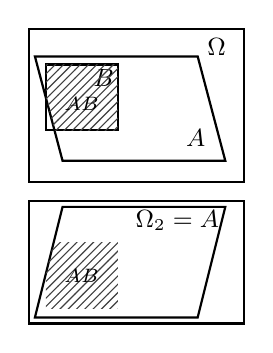
\begin{tikzpicture}[scale=0.78,every node/.style={font=\small}]
    % ---------- 上：样本空间 Ω ----------
    \draw[thick] (0,0) rectangle (3.5,2.5);
    \node[fill=white,inner sep=1pt] at (3.06,2.20) {$\Omega$};
    % 事件 A（斜四边形）
    \draw[thick] (0.55,0.35) -- (3.20,0.35) -- (2.75,2.05) -- (0.10,2.05) -- cycle;
    \node at (2.72,0.72) {$A$};
    % 事件 B（左上矩形）
    \draw[thick] (0.28,0.85) -- (1.45,0.85) -- (1.45,1.92) -- (0.28,1.92) -- cycle;
    \node[fill=white,inner sep=0.6pt] at (1.22,1.70) {$B$};
    % AB 交集（斜四边形 ∩ 矩形），阴影填充
    \begin{scope}
      \clip (0.55,0.35) -- (3.20,0.35) -- (2.75,2.05) -- (0.10,2.05) -- cycle;
      \fill[pattern=north east lines,pattern color=black!75]
        (0.28,0.85) rectangle (1.45,1.92);
    \end{scope}
    \node at (0.86,1.28) {\scriptsize $AB$};
    % ---------- 下：条件样本空间 Ω₂ = A ----------
    \draw[thick] (0,-2.30) rectangle (3.5,-0.30);
    \node[fill=white,inner sep=1pt] at (2.42,-0.62) {$\Omega_2=A$};
    \draw[thick] (0.10,-2.20) -- (2.75,-2.20) -- (3.20,-0.40) -- (0.55,-0.40) -- cycle;
    \begin{scope}
      \clip (0.10,-2.20) -- (2.75,-2.20) -- (3.20,-0.40) -- (0.55,-0.40) -- cycle;
      \fill[pattern=north east lines,pattern color=black!75]
        (0.28,-2.05) rectangle (1.45,-0.98);
    \end{scope}
    \node at (0.86,-1.52) {\scriptsize $AB$};
  \end{tikzpicture}
  \vspace{-6pt}
  \caption{条件事件及其集合表示}
  \label{fig:1.1}
\end{wrapfigure}

独立的概念用于描述事件的发生不依赖于条件的特性\nobreak，即 $P(B\,|\,A)=P(B)$\nobreak。因此\nobreak，事件 $A$ 与 $B$ 独立（Independent\nobreak）等价地定义为
\[
P(AB)=P(A)P(B)
\]

多个事件 $A_1,A_2,\cdots,A_n$ 彼此独立的定义为\nobreak：若对于任意的 $m\ (1<m\leqslant n)$ 与 $m$ 个任意整数\nobreak：$1\leqslant k_1<k_2<\cdots<k_m\leqslant n$\nobreak，满足
\begin{equation}
P\bigl(A_{k_1}A_{k_2}\cdots A_{k_m}\bigr)=P\bigl(A_{k_1}\bigr)P\bigl(A_{k_2}\bigr)\cdots P\bigl(A_{k_m}\bigr)
\label{eq:1.3}
\end{equation}
则称 $A_1,A_2,\cdots,A_n$ 彼此独立\nobreak。可见多个事件的独立要求它们两两独立\nobreak，三三独立\nobreak，以及任意 $m\ (\leqslant n)$ 个都独立\nobreak。

\bhead{3.\ 基本性质与事件运算}

基于公理\nobreak，容易导出事件概率的如下基本性质\nobreak：

\begin{citemize}
  \item ① $P(\varnothing)=0$\nobreak；
  \item ② $0\leqslant P(A)\leqslant 1$\nobreak；

% =====================================================================
%  frag_A.tex  ——  书 p.3 – p.6 （PDF 017–020）
%  承接书 p.2 末尾：\bhead{3.\ 基本性质与事件运算} 的 ① ② 两条
% =====================================================================

  \item ③ $P(A)\leqslant P(B)$\nobreak，如果 $A\subseteq B$\nobreak；
  \item ④ $P(AB)\leqslant P(A)\leqslant P(A\cup B)$\nobreak。
\end{citemize}

样本空间与事件的数学描述都是集合\nobreak，因此\nobreak，事件的运算是集合的运算\nobreak。事件的基本运算包括\nobreak：非\nobreak、加（或\nobreak）\nobreak、减\nobreak、乘（与\nobreak）及除（条件\nobreak）\nobreak，对应的概率关系如下\nobreak：

\begin{citemize}
  \item ① $P\bigl(\overline{A}\bigr)=1-P(A)$
  \item ② $\begin{aligned}[t]
        P(A\cup B)&=P(A)+P(B)-P(AB)\\
        &=P(A)+P(B)\quad(\text{如果彼此互斥})
        \end{aligned}$
  \item ③ $\begin{aligned}[t]
        P(A-B)&=P\bigl(A\cap\overline{B}\bigr)=P(A)-P(AB)\\
        &=P(A)-P(B)\quad(\text{如果 $B\subseteq A$})
        \end{aligned}$
  \item ④ $\begin{aligned}[t]
        P(AB)&=P(A)P(B\mid A),\quad P(A)>0\\
        &=P(B)P(A\mid B),\quad P(B)>0\\
        &=P(A)P(B)\quad(\text{如果彼此独立})
        \end{aligned}$
  \item ⑤ $P(B\mid A)=P(AB)/P(A),\quad P(A)>0$
\end{citemize}

通过文氏图（Venn Diagram\nobreak）可以形象化地理解概率的基本性质\nobreak、事件运算及其对应概率的运算\nobreak，如图~\ref{fig:1.2} 所示\nobreak。

\begin{figure}[htbp]
  \centering
  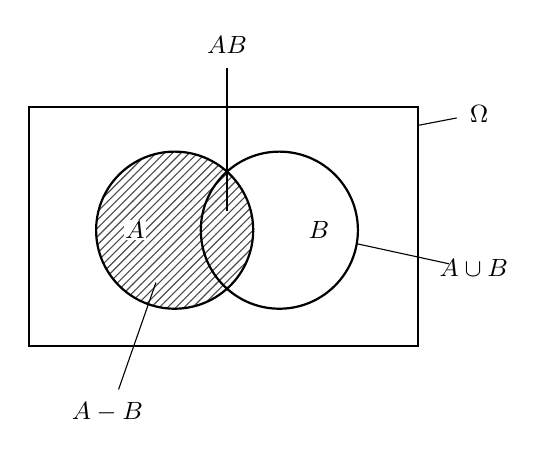
\begin{tikzpicture}[scale=0.95,every node/.style={font=\small}]
    % ---------- 样本空间 Ω ----------
    \draw[thick] (0,0) rectangle (5.2,3.2);
    % 事件 A（左圆，阴影填充）
    \fill[pattern=north east lines,pattern color=black!70] (1.95,1.55) circle (1.05);
    \draw[thick] (1.95,1.55) circle (1.05);
    % 事件 B（右圆）
    \draw[thick] (3.35,1.55) circle (1.05);
    % 圆内标号
    \node[fill=white,inner sep=0.6pt] at (1.42,1.55) {$A$};
    \node at (3.88,1.55) {$B$};
    % AB 标注（上方引出线指到交集）
    \draw (2.65,3.72) -- (2.65,1.80);
    \node at (2.65,4.02) {$AB$};
    % A∪B 标注（右侧引出线指到 B 的右弧）
    \draw (5.62,1.10) -- (4.38,1.37);
    \node at (5.95,1.05) {$A\cup B$};
    % A-B 标注（下方引出线指到 A 中不属于 B 的部分）
    \draw (1.20,-0.58) -- (1.70,0.85);
    \node at (1.05,-0.88) {$A-B$};
    % Ω 标注
    \draw (5.20,2.95) -- (5.72,3.05);
    \node at (6.02,3.10) {$\Omega$};
  \end{tikzpicture}
  \caption{文氏图}
  \label{fig:1.2}
\end{figure}

事件的反复运算生成各种新的事件\nobreak，各种不同事件的总体构成一个事件集合\nobreak，称为事件域 $F$\nobreak。样本空间\nobreak、事件和概率是概率理论的三个最基本的概念\nobreak。

\begin{examplebox}
\textbf{例1.1}\quad 分析掷均匀硬币问题\nobreak。

\textbf{解}\quad 掷币试验的基本结果是\nobreak：$H$ — 正面\nobreak，$T$ — 反面\nobreak。因此有

（1\nobreak）样本空间\nobreak：$\Omega=\{H,T\}$\nobreak。

（2\nobreak）事件域\nobreak：$F=\bigl\{\{H\},\{T\},\varnothing,\Omega\bigr\}$\nobreak。

（3\nobreak）由硬币的均匀特性可得\nobreak，$P\{H\}=P\{T\}=0.5$\nobreak；而且 $P\{\varnothing\}=0$\nobreak，$P\{\Omega\}=1$\nobreak。

\textbf{例1.2}\quad 有 $N$ 个格子排为一列\nobreak，将一只小球随机地放入其中任一格子\nobreak。对于 $k\in[1,N]$\nobreak，求\nobreak：

（1\nobreak）小球放入第 $k$ 号格子的概率\nobreak。

（2\nobreak）前 $k$ 个格子中有小球的概率\nobreak。

\textbf{解}\quad 因为是等概的\nobreak，显然
\[
P(\text{小球放入任一格子})=1/N
\]
又因为小球放入各个格子是互斥的\nobreak，于是有
\[
P(\text{小球放入任意}k\text{个格子})=k/N
\]
\end{examplebox}

基于概率论解决实际问题的原则思路是\nobreak：首先为问题设计随机试验模型\nobreak，确定其样本空间 $\Omega$\nobreak，然后合理地假设其中某些基本事件的概率\nobreak，再由它们推导出我们感兴趣的事件概率与特性\nobreak，从而解决所关心的问题\nobreak。

\bhead{4.\ 几个基本公式}
概率论中\nobreak，有下面几个重要的公式\nobreak。

\bhead{（1\nobreak）链式法则}
\begin{equation}
P(A_1A_2\cdots A_n)=P(A_1)P(A_2\mid A_1)P(A_3\mid A_1A_2)\cdots P(A_n\mid A_1A_2\cdots A_{n-1})
\label{eq:1.4}
\end{equation}
式中\nobreak，$P(A_1),P(A_1A_2),\cdots,P(A_1A_2\cdots A_{n-1})>0$\nobreak。易见\nobreak，链式法则是反复运用条件概率定义的结果\nobreak。

\bhead{（2\nobreak）全概率公式}
事件组 $A_i,i=1,2,\cdots,n$\nobreak，若满足\nobreak：
\[
\forall i\neq j,\quad A_iA_j=\varnothing;\qquad \bigcup_{i=1}^{n}A_i=\Omega
\]
则称该事件组为样本空间的一个完备事件组或分割（Partition\nobreak）\nobreak。完备事件组是既彼此互斥又可以完整地拼成 $\Omega$ 的事件组\nobreak。

若 $A_i,i=1,2,\cdots,n$\nobreak，是完备组\nobreak，任取另外一个事件 $B$\nobreak，有
\begin{equation}
P(B)=\sum_{i=1}^{n}P(B\mid A_i)P(A_i)
\label{eq:1.5}
\end{equation}
该式称为全概率公式\nobreak。

易见上式等价于 $P(B)=\sum\limits_{i=1}^{n}P(A_iB)$\nobreak，其中各个 $A_iB$ 是图~\ref{fig:1.3} 中 $B$ 的局部子块\nobreak，它们彼此互斥\nobreak。于是\nobreak，上式可由概率公理的可加性得出\nobreak。形象地讲\nobreak，全概率公式表明\nobreak：“全部”的概率是各种（互斥的\nobreak）“部分”的概率按比例构成的\nobreak。

\begin{figure}[htbp]
  \centering
  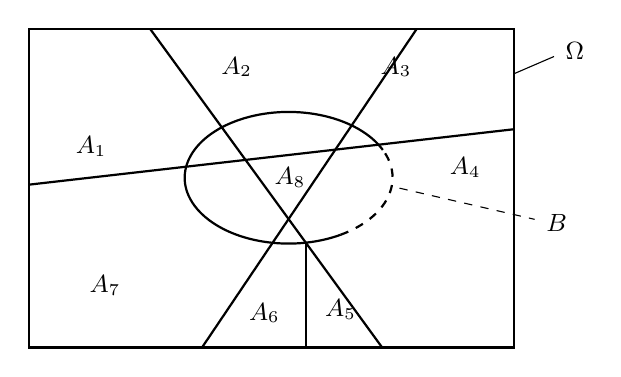
\begin{tikzpicture}[scale=0.88,every node/.style={font=\small}]
    % ---------- 样本空间 Ω ----------
    \draw[thick] (0,0) rectangle (7,4.6);
    % 分割线：三条两两相交的直线 + 一条从边界引到 L2 的线段
    \draw[thick] (0,2.35) -- (7,3.15);          % L1
    \draw[thick] (1.75,4.6) -- (5.1,0);         % L2
    \draw[thick] (2.5,0) -- (5.6,4.6);          % L3
    \draw[thick] (4.0,0) -- (4.0,1.5105);       % L4（把底部区域一分为二\nobreak）
    % ---------- 事件 B（椭圆，右下弧用虚线） ----------
    \draw[thick,dashed] (4.5000,1.6273) arc[start angle=-60,end angle=25,x radius=1.5,y radius=0.95];
    \draw[thick] (5.1095,2.8514) arc[start angle=25,end angle=300,x radius=1.5,y radius=0.95];
    % ---------- 各分割块标号 ----------
    \node at (0.90,2.90) {$A_1$};
    \node at (3.00,4.05) {$A_2$};
    \node at (5.30,4.05) {$A_3$};
    \node at (6.30,2.60) {$A_4$};
    \node at (4.50,0.55) {$A_5$};
    \node at (3.40,0.50) {$A_6$};
    \node at (1.10,0.90) {$A_7$};
    \node at (3.77,2.45) {$A_8$};
    % ---------- B 与 Ω 的标注 ----------
    \draw[dashed] (5.35,2.30) -- (7.30,1.85);
    \node at (7.62,1.80) {$B$};
    \draw (7.00,3.95) -- (7.58,4.20);
    \node at (7.88,4.28) {$\Omega$};
  \end{tikzpicture}
  \caption{全概率公式}
  \label{fig:1.3}
\end{figure}

\bhead{（3\nobreak）贝叶斯（Bayes\nobreak）公式}
若 $A_i,i=1,2,\cdots,n$\nobreak，是完备组\nobreak，任取另外一个事件 $B$\nobreak，有
\begin{equation}
P(A_k\mid B)=\frac{P(A_k)P(B\mid A_k)}{\sum\limits_{i=1}^{n}P(B\mid A_i)P(A_i)},\quad k=1,2,\cdots,n
\label{eq:1.6}
\end{equation}
易见\nobreak，上式右边的分子与分母分别为
\[
P(A_k)P(B\mid A_k)=P(A_kB),\qquad \sum_{i=1}^{n}P(B\mid A_i)P(A_i)=P(B)
\]
因此\nobreak，式（1.6\nobreak）本质上源于条件概率的定义\nobreak。

贝叶斯公式在研究因果推测\nobreak、信息传输与检测等问题中有着重要的应用\nobreak。通常将各个因事件概率 $P(A_i)$ 称为先验概率（Priori Probability\nobreak）\nobreak，它是观察事件 $B$ 出现与否的实验之前已存在的\nobreak；将条件概率 $P(B\mid A_k)$ 称为转移概率（Transition Probability\nobreak）\nobreak，它是第 $k$ 个因事件转移成（或引起\nobreak）事件 $B$ 的概率\nobreak；而将观察到 $B$ 出现之后\nobreak，条件概率 $P(A_k\mid B)$ 称为后验概率（Posteriori Probability\nobreak）\nobreak。

思考一下因果推测问题\nobreak：$A_i$ 是 $n$ 个原因事件\nobreak，$B$ 是某种结果事件\nobreak；各原因的概率是先验概率\nobreak，由原因引起结果的概率是转移概率\nobreak，而知道结果后推测起因的概率就是后验概率\nobreak。贝叶斯公式正是基于结果 $B$ 推测某种起因 $A_k$ 的可能性的方法\nobreak。

\begin{examplebox}
\textbf{例1.3}\quad 在二元传输或检测中\nobreak，假定二元消息表示为 0 与 1\nobreak，记为 $X$\nobreak，其先验概率分别为 $P\{X=0\}=0.9$\nobreak，$P\{X=1\}=0.1$\nobreak，传输可靠性为 80\%\nobreak。问\nobreak：收到 1 时\nobreak，真正发送的消息是什么\nobreak？

\textbf{解}\quad 由于传输并非绝对可靠\nobreak，不论发送的是 0 或 1\nobreak，接收到的消息可能为 0\nobreak，也可能为 1\nobreak，记为 $Y$\nobreak。如图~\ref{fig:1.4} 所示\nobreak，问题实际上是要求回答“$Y=1$ 条件下\nobreak，$X$ 到底是什么\nobreak？”\nobreak，这需要比较 $P\{X=0\mid Y=1\}$ 与 $P\{X=1\mid Y=1\}$ 的大小\nobreak。

根据贝叶斯公式可得
\[
P\{X=0\mid Y=1\}=\frac{0.9\times 0.2}{0.9\times 0.2+0.1\times 0.8}=\frac{9}{13}
\]
\[
P\{X=1\mid Y=1\}=\frac{0.1\times 0.8}{0.9\times 0.2+0.1\times 0.8}=\frac{4}{13}
\]

\begin{center}
  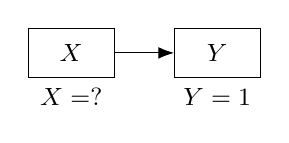
\begin{tikzpicture}[scale=0.95,every node/.style={font=\small}]
    \draw (0,0) rectangle (1.15,0.66);
    \node at (0.575,0.33) {$X$};
    \draw[-{Latex[length=2mm]}] (1.15,0.33) -- (1.95,0.33);
    \draw (1.95,0) rectangle (3.10,0.66);
    \node at (2.525,0.33) {$Y$};
    \node at (0.575,-0.26) {$X=?$};
    \node at (2.525,-0.26) {$Y=1$};
  \end{tikzpicture}

  \smallskip
  \captionof{figure}{二元传输系统}\label{fig:1.4}
\end{center}

由于 $P\{X=0\mid Y=1\}>P\{X=1\mid Y=1\}$\nobreak，收到的虽然是 1\nobreak，但合理的估计仍然是“原本发送的是 0”\nobreak，尽管传输可靠性高达 80\%\nobreak。这样一来\nobreak，不管接收到 0 或 1\nobreak，我们总是“赌”发送的是 0\nobreak。这样做当然可能出错\nobreak，但它是最为“理智”的选择\nobreak。这是因为在源端\nobreak，消息 1 本身“太稀有了”\nobreak，发送它的概率不大\nobreak。因此\nobreak，这个 1 更可能是发送 0 时错误产生的\nobreak。
\end{examplebox}

\subsection{随机变量}
概率论中的样本空间与事件等都是一般意义下的集合\nobreak，为了更加有效地进行讨论与分析\nobreak，我们希望将原来的集合描述形式转换为实数描述形式\nobreak，因为在实数域上存在着丰富的数学分析方法与结果\nobreak。为此\nobreak，设计一个从样本空间向实数域的映射\nobreak，将样本点映射为实数值\nobreak，将事件映射为实数集合\nobreak，这便产生了随机变量\nobreak。

在样本空间 $\Omega$ 上定义一个单值实函数 $X(\xi)$\nobreak，称为随机变量（random variable\nobreak，常缩写为 r.v.\nobreak）\nobreak。并规定\nobreak：任取实数 $x$\nobreak，用 $\{X(\xi)\leqslant x\}$ 的概率来描述 $X(\xi)$ 的概率特性\nobreak，记为
\begin{equation}
F_X(x)=P\{X(\xi)\leqslant x\}
\label{eq:1.7}
\end{equation}
称它为 $X$ 的概率分布函数（Probability Distribution Function\nobreak）或概率累积分布函数（Probability Cumulative Distribution Function\nobreak）\nobreak，简称为分布函数\nobreak。

定义随机变量 $X(\xi)$ 时\nobreak，不仅关心它取什么值\nobreak，而且关心它取值的概率大小\nobreak。定义中的 $\{X(\xi)\leqslant x\}$ 是 $\{\xi: X(\xi)\leqslant x\}$ 的缩写\nobreak，它本质上是样本空间上某些样本点的集合\nobreak，具体讲\nobreak，是随机变量的值不超过 $x$ 所对应的样本点的集合\nobreak，它是一个事件\nobreak，而非普通的实数集合\nobreak。为了书写简便\nobreak，常省略括号及其中的 $\xi$\nobreak，将随机变量简记为 $X$\nobreak。

分布函数 $F_X(x)$ 的下标指出它所关注的随机变量是 $X$\nobreak，常常可以省略\nobreak；而自变量 $x$ 是确定变量\nobreak，指示取值的位置\nobreak。由概率公理与性质容易得出\nobreak，分布函数具有如下基本性质\nobreak：

① $F(-\infty)=0$\nobreak，$F(+\infty)=1$\nobreak；

② $F(x)$ 是右连续的单调非降函数\nobreak，即
\[
F(x_1)\leqslant F(x_2),\quad x_1<x_2;\qquad F\bigl(x^+\bigr)=F(x)
\]

③ 在随机变量上\nobreak，事件对应于实数集合\nobreak，常用区间描述\nobreak。基本区间事件的概率计算公式为
\[
P\{x_1<x\leqslant x_2\}=F(x_2)-F(x_1)
\]
\[
P\{x_1\leqslant x\leqslant x_2\}=P\{x_1<x\leqslant x_2\}+P(x=x_1)=F(x_2)-F\bigl(x_1^-\bigr)
\]
\[
P\{x_1<x<x_2\}=P\{x_1<x\leqslant x_2\}-P(x=x_2)=F\bigl(x_2^-\bigr)-F(x_1)
\]
\[
P(X=x)=F(x)-F\bigl(x^-\bigr)
\]
式中\nobreak，$F\bigl(x^-\bigr)$ 与 $F\bigl(x^+\bigr)$ 分别表示 $F(x)$ 在 $x$ 处的左\nobreak、右极限\nobreak。

实用中\nobreak，$X$ 只会有三种类型\nobreak，由它们的分布函数反映出来\nobreak：

① 连续型\nobreak：$F(x)$ 是连续取值的\nobreak。由于它有无限多种取值而所有取值的概率之和为 1\nobreak，显然\nobreak，它取任何单个实数值的概率均为零\nobreak，即 $\forall x$ 有 $P(X=x)=0$\nobreak。

② 离散型\nobreak：$F(x)$ 仅含有跳跃型间断点\nobreak。这些间断点是可列的\nobreak，记为 $\{x_i\}$\nobreak；显然\nobreak，$X$ 只能取这些点\nobreak，或者说\nobreak，$X$ 仅在这些点上具有非零的概率\nobreak，记为 $\{p_i\}$\nobreak。因此
\[
P(X=x_i)=p_i=F(x_i)-F\bigl(x_i^-\bigr)\qquad (i\ \text{为整数})
\]
称为 $X$ 的分布律（或分布列\nobreak）（Distribution Law\nobreak）\nobreak。并有 $\sum\limits_{i}p_i=1,p_i\geqslant 0$\nobreak。

③ 混合型\nobreak：这时 $F(x)$ 既有连续的部分也有间断点\nobreak，是上面两种形式的组合\nobreak。

可见\nobreak，分布函数可能含有间断点\nobreak，但它们必定是跳跃型的\nobreak。

$X$ 的概率密度函数（Probability Density Function\nobreak）（简称密度函数\nobreak）定义为其分布函数的导数\nobreak，即
\begin{equation}
f(x)=\frac{\dif}{\dif x}F(x)
\label{eq:1.8}
\end{equation}
密度函数的基本性质为\nobreak：

① 非负性与归一性\nobreak：$f(x)\geqslant 0$\nobreak，$\int_{-\infty}^{+\infty}f(x)\dif x=1$

② 区间 $A$ 上的概率计算公式\nobreak：$P\{X\in A\}=\int_{A}f(x)\dif x$

$f(x)$ 的定义涉及到求导运算\nobreak，当 $F(x)$ 不连续时\nobreak，我们引入阶跃函数 $u(x)$ 与冲激函数 $\delta(x)$ 来表示 $F(x)$ 和 $f(x)$\nobreak。定义
\begin{equation}
u(x)=\begin{cases}1, & x\geqslant 0\\ 0, & x<0\end{cases};\qquad \delta(x)=\frac{\dif}{\dif x}u(x)
\label{eq:1.9}
\end{equation}
这样\nobreak，即使在 $F(x)$ 的间断处\nobreak，我们仍可认为其（广义\nobreak）导数存在\nobreak，于是\nobreak，密度函数存在\nobreak。

极端的情况是\nobreak，分布律为 $P(X=x_i)=p_i$ 的离散型随机变量\nobreak，其分布函数为
\begin{equation}
F(x)=\sum_{i}p_iu(x-x_i)\qquad (i\ \text{为整数})
\label{eq:1.10}
\end{equation}
密度函数为
\begin{equation}
f(x)=\sum_{i}p_i\delta(x-x_i)\qquad (i\ \text{为整数})
\label{eq:1.11}
\end{equation}
式中\nobreak，取值位置对应 $u(\ )$ 与 $\delta(\ )$ 自变量的偏移量\nobreak，取值概率对应前面的幅值\nobreak。

\begin{examplebox}
\textbf{例1.4}\quad 均匀骰子实验\nobreak。定义随机变量 $X$ 为骰子顶面的编号\nobreak，取值为 $\{1,2,3,4,5,6\}$\nobreak。

显然 $X$ 是离散型的\nobreak，其概率特性通常用分布律描述最为方便\nobreak，即
\[
P(X=i)=1/6\qquad (i=1,2,\cdots,6)
\]
或者采用表~\ref{tab:1.1} 进行表示\nobreak，直观\nobreak、清楚\nobreak。

\begin{center}
  \captionof{table}{均匀骰子实验中\nobreak，随机变量的分布律}\label{tab:1.1}

  \smallskip
  \begin{tabular}{lcccccc}
    \toprule
    状态: $\{x_i\}$ & 1 & 2 & 3 & 4 & 5 & 6 \\
    概率: $\{p_i\}$ & $1/6$ & $1/6$ & $1/6$ & $1/6$ & $1/6$ & $1/6$ \\
    \bottomrule
  \end{tabular}
\end{center}

但使用分布函数与概率密度函数可以统一地描述各型随机变量的概率特性\nobreak，由式（1.10\nobreak）与式（1.11\nobreak）可得
\[
F(x)=\sum_{i=1}^{6}\frac{1}{6}u(x-i),\quad\text{或}\quad f(x)=\sum_{i=1}^{6}\frac{1}{6}\delta(x-i)
\]
\end{examplebox}

% EQNUMBERS: 1.4, 1.5, 1.6, 1.7, 1.8, 1.9, 1.10, 1.11  （连续，无跳号）

% =====================================================================
%  frag_B.tex  —— 《随机信号分析（第5版）》书 p.7 – p.9
%  内容：1.2 多维随机变量与条件随机变量 / 1.2.1 多维随机变量
%        例1.5、例1.6、例1.7（开头）
%  本段产出的原书公式编号：(1.12) (1.13) (1.14) (1.15) (1.16) (1.17)，连续无跳号。
%  ⚠ 图 1.5 是跨书 p.6–p.7 的整幅插图，其图注落在书 p.7 顶部；
%    若 frag_A.tex 已排出该图（\label{fig:1.5}），合并时必须删除本文件的图 1.5 块，
%    否则重号 + 重复插图。见下方该 figure 环境的注释。
% =====================================================================

% !!! 郑重提醒：本 figure 块仅为“兜底”。跨页图 1.5 的正文引出语（“如图 1.5 所示。”）
%     印在书 p.6 末行，属于 frag_A.tex 的范围；若 frag_A.tex 已含 \label{fig:1.5}，
%     请删除下面整块，只保留紧随其后的正文行。
\begin{figure}[htbp]
  \centering
  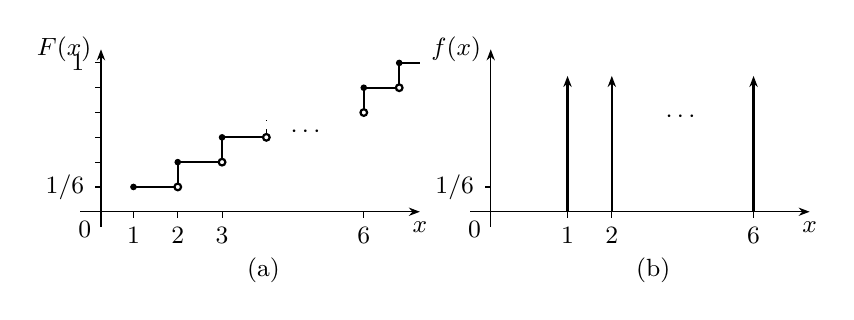
\begin{tikzpicture}[scale=0.75,every node/.style={font=\small}]
    % ---------------- (a) 分布函数 F(x) ----------------
    \begin{scope}
      \draw[-{Stealth[length=4pt]}] (-0.35,0) -- (5.4,0) node[below] {$x$};
      \draw[-{Stealth[length=4pt]}] (0,-0.25) -- (0,2.75) node[left] {$F(x)$};
      \node[below left] at (0,0) {$0$};
      % 纵轴刻度：1/6, 2/6, ..., 1
      \foreach \k in {1,...,6}{
        \draw (0,\k*0.42) -- (-0.10,\k*0.42);
      }
      \node[left] at (-0.12,0.42) {$1/6$};
      \node[left] at (-0.12,2.52) {$1$};
      % 阶梯曲线（1..6 点等概率 1/6）
      \draw[thick] (0.55,0.42) -- (1.30,0.42);
      \draw[thick] (1.30,0.84) -- (2.05,0.84);
      \draw[thick] (2.05,1.26) -- (2.80,1.26);
      % 中间省略段
      \draw[dashed] (2.80,1.26) -- (2.80,1.55);
      \node at (3.50,1.35) {$\cdots$};
      \draw[dashed] (4.45,1.68) -- (4.45,2.10);
      \draw[thick] (4.45,2.10) -- (5.05,2.10);
      \draw[thick] (5.05,2.52) -- (5.40,2.52);
      % 跳跃竖线
      \draw[thick] (1.30,0.42) -- (1.30,0.84);
      \draw[thick] (2.05,0.84) -- (2.05,1.26);
      \draw[thick] (4.45,1.68) -- (4.45,2.10);
      \draw[thick] (5.05,2.10) -- (5.05,2.52);
      % 实心/空心端点
      \foreach \p in {(0.55,0.42),(1.30,0.84),(2.05,1.26),(4.45,2.10),(5.05,2.52)}{
        \fill \p circle (1.6pt);
      }
      \foreach \p in {(1.30,0.42),(2.05,0.84),(2.80,1.26),(4.45,1.68),(5.05,2.10)}{
        \draw[fill=white,thick] \p circle (1.6pt);
      }
      % 横轴刻度
      \foreach \x/\t in {0.55/1,1.30/2,2.05/3,4.45/6}{
        \draw (\x,0) -- (\x,-0.10);
        \node[below] at (\x,-0.10) {$\t$};
      }
      \node[below] at (2.75,-0.62) {(a)};
    \end{scope}
    % ---------------- (b) 密度函数 f(x) ----------------
    \begin{scope}[shift={(6.6,0)}]
      \draw[-{Stealth[length=4pt]}] (-0.35,0) -- (5.4,0) node[below] {$x$};
      \draw[-{Stealth[length=4pt]}] (0,-0.25) -- (0,2.75) node[left] {$f(x)$};
      \node[below left] at (0,0) {$0$};
      \draw (0,0.42) -- (-0.10,0.42);
      \node[left] at (-0.12,0.42) {$1/6$};
      % 冲激（箭头）位置
      \foreach \x in {1.30,2.05}{
        \draw[-{Stealth[length=4pt]},thick] (\x,0) -- (\x,2.30);
      }
      \draw[-{Stealth[length=4pt]},thick] (4.45,0) -- (4.45,2.30);
      \node at (3.25,1.60) {$\cdots$};
      \foreach \x/\t in {1.30/1,2.05/2,4.45/6}{
        \draw (\x,0) -- (\x,-0.10);
        \node[below] at (\x,-0.10) {$\t$};
      }
      \node[below] at (2.75,-0.62) {(b)};
    \end{scope}
  \end{tikzpicture}
  \caption{均匀骰子试验中\nobreak，随机变量的分布函数与密度函数}
  \label{fig:1.5}
\end{figure}

如图 1.5 所示\nobreak。（本题中\nobreak，定义该随机变量时\nobreak，其实还隐含规定 $X$ 取其他实数值的概率为零\nobreak）\nobreak。

随机变量不同于普通变量就在于其“随机性”\nobreak，而随机性表现为以下两点\nobreak：

\begin{citemize}
  \item ① 变量可以有多个取值\nobreak，并且永远不能预知它到底会取哪个值\nobreak；
  \item ② 变量取值是有规律的\nobreak，这种规律是“宏观”的\nobreak，用概率特性来明确表述\nobreak。
\end{citemize}

因此\nobreak，凡是讨论随机变量就必然要联系到它的取值范围与概率特性\nobreak。常用的概率特性\nobreak，如正态分布\nobreak、均匀分布\nobreak、0-1 分布等\nobreak，在初等概率论中已学习过\nobreak。1.6 节将详细列出\nobreak。

在描述随机变量的概率特性时\nobreak，我们注意到\nobreak：

\begin{citemize}
  \item ① 对于离散变量\nobreak，采用取值概率来描述是最直观与最方便的\nobreak，这便是分布律\nobreak；
  \item ② 对于连续变量或混合变量的连续部分\nobreak，由于任何单个取值的概率都为零\nobreak，因此\nobreak，我们只好采用分布函数 $F_X(x)$ 进行描述\nobreak，其中自变量 $x$ 不是随机变量\nobreak，而是（确定的\nobreak）指示参量\nobreak。$F_X(x)$ 指明直到 $x$ 处的累积概率\nobreak，即 $P\{X\leqslant x\}$\nobreak；
  \item ③ 尽管连续变量或混合变量的连续部分取值的概率都为零\nobreak，但不同位置处的概率密度（或“强度”\nobreak）是不同的\nobreak，这种规律便是密度函数 $f_X(x)$\nobreak，它同样全面地表示了随机变量的概率特性\nobreak。实际上\nobreak，对于连续变量采用概率密度函数通常是最方便的\nobreak。基于概率密度函数\nobreak，我们很容易运用积分运算计算各种事件的概率\nobreak。
\end{citemize}

随机变量的定义中采用了分布函数\nobreak，因为它在数学上具有更好的普适性\nobreak。

\section{多维随机变量与条件随机变量}

\subsection{多维随机变量}

多个随机变量放在一起\nobreak，构成 $n$ 维随机变量（或向量\nobreak）\nobreak，记为 $(X_1,\cdots,X_n)$\nobreak。它们的概率特性由 $n$ 维（或 $n$ 元\nobreak）联合概率分布与密度函数描述\nobreak，分别定义为
\begin{equation}
F_{X_1X_2\cdots X_n}(x_1,x_2,\cdots,x_n)=P\{X_1\leqslant x_1,\cdots,X_n\leqslant x_n\}
\label{eq:1.12}
\end{equation}
\begin{equation}
f_{X_1X_2\cdots X_n}(x_1,x_2,\cdots,x_n)=\frac{\partial^n}{\partial x_1\cdots\partial x_n}F_{X_1X_2\cdots X_n}(x_1,x_2,\cdots,x_n)
\label{eq:1.13}
\end{equation}

联合概率特性包含了分量随机变量各自的（边缘\nobreak）概率特性与相互间“交叉”的概率特性\nobreak。它们的基本性质与前面的相仿\nobreak。

以二维为例\nobreak，分布函数反映了直到 $(x,y)$ 处的联合累积概率\nobreak，它有下面的性质\nobreak：

\begin{citemize}
  \item ① $F_{XY}(x,-\infty)=0$\nobreak，$F_{XY}(-\infty,y)=0$\nobreak，$F_{XY}(+\infty,+\infty)=1$\nobreak；
  \item ② $F_{XY}(x,y)$ 是 $x$ 或 $y$ 的单调非减函数\nobreak；
  \item ③ $P\{a<X\leqslant b;c<Y\leqslant d\}=F_{XY}(b,d)-F_{XY}(a,d)-F_{XY}(b,c)+F_{XY}(a,c)$\nobreak，如图 1.6 所示\nobreak。
  \item ④ 边缘概率分布为
\end{citemize}
\[
F_X(x)=F_{XY}(x,+\infty),\qquad F_Y(y)=F_{XY}(+\infty,y)
\]

二维概率密度函数反映了在 $(x,y)$ 处的联合概率“强度”\nobreak，它具有下面的基本性质\nobreak：

\begin{citemize}
  \item ① 非负与归一化\nobreak：$f_{XY}(x,y)\geqslant 0$\nobreak，$\displaystyle\int_{-\infty}^{+\infty}\int_{-\infty}^{+\infty}f_{XY}(x,y)\dif x\dif y=1$
  \item ② 区域 $D$ 上的概率\nobreak：$\displaystyle P\{(x,y)\in D\}=\iint_D f_{XY}(x,y)\dif x\dif y$
  \item ③ 边缘概率密度为\nobreak：
\end{citemize}
% 说明：原书式(1.14) 为一行两式（f_X 与 f_Y 并排）。本页版心仅 132mm，
% 并排会超宽 14pt，故拆成两行（gathered），内容与原书完全一致。
\[
\begin{gathered}
f_X(x)=\frac{\dif}{\dif x}F_X(x)=\int_{-\infty}^{+\infty}f_{XY}(x,y)\dif y,\\[4pt]
f_Y(y)=\frac{\dif}{\dif y}F_Y(y)=\int_{-\infty}^{+\infty}f_{XY}(x,y)\dif x
\end{gathered}
\]

% ---------------- 图 1.6 ----------------
\begin{figure}[htbp]
  \centering
  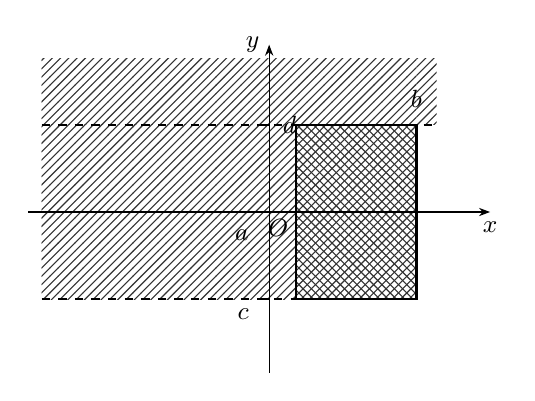
\begin{tikzpicture}[scale=0.85,every node/.style={font=\small}]
    % 区域划分坐标：a=0.40, b=2.20, c=-1.30, d=1.30
    % (1) 斜线阴影：x<=a 且 c<y<=d（左侧长条）
    \fill[pattern=north east lines,pattern color=black!80]
      (-3.40,1.30) rectangle (0.40,-1.30);
    % (2) 交叉阴影：a<x<=b 且 c<y<=d（目标矩形区域）
    \begin{scope}
      \clip (0.40,-1.30) rectangle (2.20,1.30);
      \fill[pattern=north east lines,pattern color=black!80]
        (0.40,-1.30) rectangle (2.20,1.30);
      \fill[pattern=north west lines,pattern color=black!80]
        (0.40,-1.30) rectangle (2.20,1.30);
    \end{scope}
    % (3) 斜线阴影：x<=b 且 y>d（顶部横条）
    \fill[pattern=north east lines,pattern color=black!80]
      (-3.40,2.30) rectangle (2.20,1.30);
    % (4) 斜线阴影：b<x 且 y>d 处的延伸（原图右上角亦为斜线，只到 b 稍右）
    \fill[pattern=north east lines,pattern color=black!80]
      (2.20,2.30) rectangle (2.50,1.30);
    % 坐标轴
    \draw[-{Stealth[length=4pt]}] (-3.60,0) -- (3.30,0) node[below] {$x$};
    \draw[-{Stealth[length=4pt]}] (0,-2.40) -- (0,2.50) node[left] {$y$};
    % 界线
    \draw[dashed] (-3.40,1.30) -- (2.50,1.30);
    \draw[dashed] (-3.40,-1.30) -- (2.20,-1.30);
    \draw[dashed] (2.20,1.30) -- (2.20,-1.30);
    % 目标矩形边框
    \draw[thick] (0.40,-1.30) rectangle (2.20,1.30);
    % 刻度
    \draw (0.40,0) -- (0.40,-0.10);
    \draw (2.20,0) -- (2.20,-0.10);
    \draw (0,1.30) -- (-0.10,1.30);
    \draw (0,-1.30) -- (-0.10,-1.30);
    % 标注（放在空白侧，避免与阴影、坐标轴重叠）
    \node[below left] at (-0.16,-0.12) {$a$};
    \node[above] at (2.20,1.42) {$b$};
    \node[below right] at (-0.16,0.04) {$O$};
    \node[right] at (0.06,1.30) {$d$};
    \node[below left] at (-0.16,-1.30) {$c$};
  \end{tikzpicture}
  \caption{$P\{a<X\leqslant b;c<Y\leqslant d\}$ 的几何表示}
  \label{fig:1.6}
\end{figure}

离散型随机向量的概率特性常常用联合分布律来描述
\begin{equation}
P\{X=x_i,Y=y_j\}=p_{ij},\qquad \sum_i\sum_j p_{ij}=1
\label{eq:1.14}
\end{equation}
从中可以清楚地看到 $(X,Y)$ 取各离散点的概率\nobreak。联合密度函数完全由如下形式的多维冲激函数组成
\begin{equation}
f_{XY}(x,y)=\sum_i\sum_j p_{ij}\delta(x-x_i,y-y_j)
\label{eq:1.15}
\end{equation}
其中\nobreak，$\delta(x,y)=\delta(x)\delta(y)$\nobreak。其联合分布函数由如下形式多维阶跃函数组成
\begin{equation}
F_{XY}(x,y)=\sum_i\sum_j p_{ij}u(x-x_i,y-y_j)
\label{eq:1.16}
\end{equation}
其中\nobreak，$u(x,y)=u(x)u(y)$\nobreak。式（1.15\nobreak）与式（1.16\nobreak）中\nobreak，随机变量取值位置对应 $u(\ )$ 与 $\delta(\ )$ 自变量的偏移量\nobreak，取值概率对应前面的幅值\nobreak。

\begin{examplebox}
\textbf{例1.5}\quad 某电子系统有部件 $A_1$ 和 $A_2$\nobreak。部件正常工作记为 $n$\nobreak，发生故障记为 $f$\nobreak，且 $P[A_1=f]=0.01$\nobreak，$P[A_2=f]=0.02$\nobreak。定义如下随机变量
\[
X_1=\begin{cases}1,&A_1=n\\ 0,&A_1=f\end{cases};\qquad
X_2=\begin{cases}1,&A_2=n\\ 0,&A_2=f\end{cases}
\]
（1\nobreak）给出观察系统工作情况的样本空间 $\Omega$ 和随机向量 $(X_1,X_2)$ 的联合样本空间 $S_J$\nobreak，并指出 $\Omega$ 和 $S_J$ 中事件的对应关系\nobreak；

（2\nobreak）计算 $(X_1,X_2)$ 的概率密度函数\nobreak。

\textbf{解}\nobreak：电子系统工作情况可由部件 $A_1$ 和 $A_2$ 的工作情况表示\nobreak。因此\nobreak，系统工作情况的样本空间为
\[
\Omega=\{(n,n),(n,f),(f,n),(f,f)\}
\]
随机变量 $X_1$ 和 $X_2$ 为实数\nobreak，因此\nobreak，联合样本空间为二维实空间中的四点\nobreak：
\[
S_J=\{(1,1),(1,0),(0,1),(0,0)\}
\]
$\Omega$ 与 $S_J$ 及其对应关系如图 1.7(a) 所示\nobreak。

若假定部件 $A_1$ 和 $A_2$ 是否正常工作的事件是彼此独立的\nobreak，则有
\[
\begin{aligned}
P[X_1=1,X_2=1]&=P[A_1=n,A_2=n]=P[A_1=n]P[A_2=n]\\
&=(1-0.01)\times(1-0.02)=0.9702
\end{aligned}
\]
如果将 $P[A_1=n,A_2=n]$ 和 $P[X_1=1,X_2=1]$ 简记为 $P\{n,n\}$\nobreak、$P\{1,1\}$\nobreak，则上式变为
\[
P\{1,1\}=P\{n,n\}=0.9702
\]
类似于上面的分析\nobreak，还有
\[
\begin{aligned}
P\{1,0\}&=P\{n,f\}=(1-0.01)\times(0.02)=0.0198\\
P\{0,1\}&=P\{f,n\}=0.01\times(1-0.02)=0.0098\\
P\{0,0\}&=P\{f,f\}=0.01\times0.02=0.0002
\end{aligned}
\]
使用二维冲激函数记号\nobreak，$(X_1,X_2)$ 的概率密度函数可以表示为
\[
\begin{aligned}
f(x_1,x_2)=\ &0.9702\delta(x_1-1,x_2-1)+0.0198\delta(x_1-1,x_2)\\
&+0.0098\delta(x_1,x_2-1)+0.0002\delta(x_1,x_2)
\end{aligned}
\]
于是\nobreak，电子系统工作情况的概率密度函数 $f(x_1,x_2)$ 的图形如图 1.7(b) 所示\nobreak。
\end{examplebox}

% ---------------- 图 1.7 ----------------
\begin{figure}[htbp]
  \centering
  \begin{tikzpicture}[scale=0.9,every node/.style={font=\small}]
    % ============ (a) 样本空间 Ω → 联合样本空间 S_J ============
    \begin{scope}
      % 左：系统状态的四个样本点
      \draw[thick] (0,0) rectangle (1.5,2.6);
      \foreach \y/\t in {2.25/{(n,n)},1.75/{(f,n)},1.25/{(n,f)},0.75/{(f,f)}}{
        \node[left] at (1.42,\y) {$\t$};
      }
      % 右：x1-x2 样本空间（正交坐标）
      \draw[-{Stealth[length=4pt]}] (3.1,0.45) -- (6.4,0.45) node[below] {$x_1$};
      \draw[-{Stealth[length=4pt]}] (4.1,0.05) -- (4.1,2.9) node[left] {$x_2$};
      % 单位刻度
      \draw (4.1,0.45) -- (4.1,0.45);
      \draw (4.75,0.45) -- (4.75,0.35);
      \node[below] at (4.75,0.34) {$1$};
      \draw (4.1,1.10) -- (4.0,1.10);
      \node[left] at (3.98,1.10) {$1$};
      \node[below left] at (4.06,0.42) {$0$};
      % 四个样本点 (0,0) (1,0) (0,1) (1,1)
      \foreach \x/\y in {4.1/0.45,4.75/0.45,4.1/1.10,4.75/1.10}{
        \fill (\x,\y) circle (1.8pt);
      }
      \node[below right] at (4.78,0.42) {\scriptsize $(1,0)$};
      \node[above left] at (4.06,1.14) {\scriptsize $(0,1)$};
      \node[above right] at (4.78,1.14) {\scriptsize $(1,1)$};
      \node[below left] at (4.06,0.40) {\scriptsize $(0,0)$};
      % 映射虚线：每个样本点对分别指向一点
      \draw[dashed] (1.50,2.25) -- (4.75,1.10);
      \draw[dashed] (1.50,1.75) -- (4.75,0.45);
      \draw[dashed] (1.50,1.25) -- (4.10,1.10);
      \draw[dashed] (1.50,0.75) -- (4.10,0.45);
      \node[below] at (2.10,-0.35) {$(X_1,X_2)$ 变换};
      \node[below] at (4.90,-0.35) {$(X_1,X_2)$ 空间\nobreak：$S_J$};
      \node[below] at (3.20,-1.00) {(a)};
    \end{scope}
    % ============ (b) 概率密度函数 ============
    \begin{scope}[shift={(7.9,0)}]
      \draw[-{Stealth[length=4pt]}] (0.20,0.20) -- (3.80,0.20) node[below] {$x_1$};
      \draw[-{Stealth[length=4pt]}] (0.20,0.20) -- (3.80,1.75) node[right] {$x_2$};
      \draw[-{Stealth[length=4pt]}] (0.20,0.20) -- (0.20,3.35) node[left] {$f(x_1,x_2)$};
      % 底面四个冲激位置：(0,0)=(1.10,0.45) (1,0)=(1.95,0.45)
      %                       (0,1)=(1.10,0.90) (1,1)=(1.95,0.90)
      \draw[thick] (1.10,0.45) -- (1.10,0.68);   % (0,0)  0.0002
      \draw[thick] (1.95,0.45) -- (1.95,1.90);   % (1,0)  0.0198
      \draw[thick] (1.10,0.90) -- (1.10,1.55);   % (0,1)  0.0098
      \draw[thick] (1.95,0.90) -- (1.95,2.95);   % (1,1)  0.9702
      \node[left] at (1.06,0.66) {\scriptsize $0.0002$};
      \node[right] at (2.00,1.92) {\scriptsize $0.0198$};
      \node[left] at (1.06,1.62) {\scriptsize $0.0098$};
      \node[right] at (2.00,2.98) {\scriptsize $0.9702$};
      % 底面网格与坐标标注
      \draw[dotted] (1.10,0.45) -- (1.95,0.45);
      \draw[dotted] (1.10,0.90) -- (1.95,0.90);
      \draw[dotted] (1.10,0.45) -- (1.10,0.90);
      \draw[dotted] (1.95,0.45) -- (1.95,0.90);
      \node[below] at (0.95,0.16) {$0$};
      \node[below] at (1.5,-0.35) {(b)};
    \end{scope}
  \end{tikzpicture}
  \caption{例1.5 图}
  \label{fig:1.7}
\end{figure}

\begin{examplebox}
\textbf{例1.6}\quad 已知随机变量 $(X,Y)$ 仅在区域 $D=\{0\leqslant x\leqslant 2,\lvert y\rvert\leqslant 2-x\}$ 上取值\nobreak，如图 1.8 所示\nobreak，并且为均匀分布\nobreak。求此二维均匀分布的 $f(x,y)$\nobreak、$f_X(x)$ 与 $f_Y(y)$\nobreak。

\textbf{解}\nobreak：由于区域 $D$ 如图 1.8 所示\nobreak，可得面积 $S=4$\nobreak，因此
\[
f(x,y)=\begin{cases}1/S,&(x,y)\in D\\[2pt] 0,&\text{其 他}\end{cases}
=\begin{cases}1/4,&(x,y)\in D\\[2pt] 0,&\text{其 他}\end{cases}
\]
利用积分可求得边缘密度函数为
\[
f_X(x)=\begin{cases}\displaystyle\int_{x-2}^{2-x}\frac{1}{4}\dif y=1-x/2,&x\in[0,2]\\[10pt] 0,&\text{其 他}\end{cases}
\]
\[
f_Y(y)=\begin{cases}\displaystyle\int_{0}^{2-y}\frac{1}{4}\dif x,&y\in[0,2]\\[10pt]
\displaystyle\int_{0}^{y+2}\frac{1}{4}\dif x,&y\in[-2,0)\\[10pt]
0,&\text{其 他}\end{cases}
=\begin{cases}\dfrac{2-\lvert y\rvert}{4},&\lvert y\rvert\leqslant 2\\[8pt] 0,&\text{其 他}\end{cases}
\]
\end{examplebox}

% ---------------- 图 1.8 ----------------
% 说明：原书图 1.8 为绕排小图（右侧、文字环绕）。这里改为普通浮动图，
% 因为 wrapfigure 会把随后的例1.7 正文行宽压到约 6.9cm，导致式(1.18)无法排下。
\begin{figure}[htbp]
  \centering
  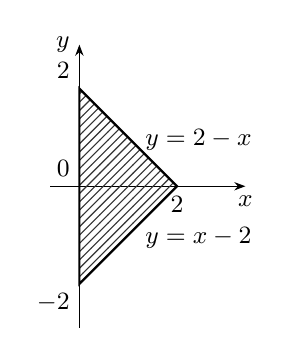
\begin{tikzpicture}[scale=0.62,every node/.style={font=\small}]
    \draw[-{Stealth[length=4pt]}] (-0.6,0) -- (3.4,0) node[below] {$x$};
    \draw[-{Stealth[length=4pt]}] (0,-2.9) -- (0,2.9) node[left] {$y$};
    % 区域 D：三角形 (0,2)-(2,0)-(0,-2)
    \begin{scope}
      \clip (0,2) -- (2,0) -- (0,-2) -- cycle;
      \fill[pattern=north east lines,pattern color=black!80] (-0.5,-2.8) rectangle (3.0,2.8);
    \end{scope}
    \draw[thick] (0,2) -- (2,0) -- (0,-2) -- cycle;
    \node[above left] at (0,2) {$2$};
    \node[below left] at (0,-2) {$-2$};
    \node[above left] at (0,0) {$0$};
    \node[below] at (2,0) {$2$};
    \node[right] at (1.15,0.95) {$y=2-x$};
    \node[right] at (1.15,-1.05) {$y=x-2$};
  \end{tikzpicture}
  \caption{区域 $D$}
  \label{fig:1.8}
\end{figure}

\begin{examplebox}
\textbf{例1.7}\quad 二维正态分布随机变量 $(X,Y)\sim N(\mu_1,\sigma_1^2;\mu_2,\sigma_2^2;\rho)$\nobreak，其联合概率密度函数为
\begin{equation}
\resizebox{\linewidth}{!}{$\displaystyle
f(x,y)=\frac{1}{2\pi\sigma_1\sigma_2\sqrt{1-\rho^2}}
\exp\Bigl\{-\frac{1}{2(1-\rho^2)}\Bigl[\Bigl(\frac{x-\mu_1}{\sigma_1}\Bigr)^2
-2\rho\frac{(x-\mu_1)(y-\mu_2)}{\sigma_1\sigma_2}
+\Bigl(\frac{y-\mu_2}{\sigma_2}\Bigr)^2\Bigr]\Bigr\}$}
\label{eq:1.17}
\end{equation}
式中\nobreak，$\mu_1$\nobreak，$\mu_2$ 为任意常数\nobreak，$\sigma_1$\nobreak，$\sigma_2$ 为正常数\nobreak，$\lvert\rho\rvert\leqslant 1$ 为常数\nobreak。求 $f_X(x)$ 与 $f_Y(y)$\nobreak。

\textbf{解}\nobreak：首先将 $f(x,y)$ 的指数部分写为

% EQNUMBERS: 1.12, 1.13, 1.14, 1.15, 1.16, 1.17

% =====================================================================
%  frag_C.tex —— 《随机信号分析（第5版）》第1章
%  覆盖书 p.10 – p.12 （PDF 第 24–26 页）
%  层级：1.2.2 条件随机变量 / 1.2.3 独立性 / 1.3 随机变量的函数 / 1.3.1 一元函数
% =====================================================================


\[
\begin{aligned}
&-\frac{\left[\left(\rho\dfrac{x-\mu_1}{\sigma_1}-\dfrac{y-\mu_2}{\sigma_2}\right)^2
+(1-\rho^2)\dfrac{(x-\mu_1)^2}{\sigma_1^2}\right]}{2(1-\rho^2)}\\[2pt]
&\qquad=-\frac{\left[y-\mu_2-\rho\dfrac{(x-\mu_1)\sigma_2}{\sigma_1}\right]^2}{2(1-\rho^2)\sigma_2^2}
-\frac{(x-\mu_1)^2}{2\sigma_1^2}
\end{aligned}
\]

则
\[
\begin{aligned}
f_X(x)&=\int_{-\infty}^{+\infty}f(x,y)\dif y\\
&=\frac{1}{\sqrt{2\pi}\sigma_1}\exp\left[\frac{-(x-\mu_1)^2}{2\sigma_1^2}\right]\\
&\qquad\times\int_{-\infty}^{+\infty}\frac{1}{\sqrt{2\pi}\sigma_2\sqrt{1-\rho^2}}
\exp\left\{-\frac{\left[y-\mu_2-\rho\dfrac{(x-\mu_1)\sigma_2}{\sigma_1}\right]^2}
{2(1-\rho^2)\sigma_2^2}\right\}\dif y
\end{aligned}
\]

对照一维正态密度函数形式\nobreak，并利用其归一性\nobreak，易知上式右边的积分项正好为 1\nobreak，因此
\[
f_X(x)=\frac{1}{\sqrt{2\pi}\sigma_1}\exp\left\{-\frac{(x-\mu_1)^2}{2\sigma_1^2}\right\}
\]

同理可得
\[
f_Y(y)=\frac{1}{\sqrt{2\pi}\sigma_2}\exp\left\{-\frac{(y-\mu_2)^2}{2\sigma_2^2}\right\}
\]

可见\nobreak，它的边缘分布分别是 $X$ 与 $Y$ 的一维正态分布\nobreak。
\end{examplebox}

注意\nobreak，在符号的书写习惯上\nobreak，采用下标指明关联的随机变量\nobreak，例如\nobreak，$F_X(\;)$\nobreak，$f_Y(\;)$ 分别是 $X$ 与 $Y$ 的分布与密度函数\nobreak。当不会发生混淆时\nobreak，也常常略去下标\nobreak，简化书写\nobreak。这时一般使用与随机变量同名的小写字母为相应自变量\nobreak。因此\nobreak，借助自变量可以帮助理解公式的确切含义\nobreak，例如\nobreak，$F(x)$\nobreak，$f(y)$\nobreak。但要特别注意的是\nobreak，自变量本质上是取值的指示变量\nobreak，它也可以用任何其他符号\nobreak，而与原随机变量没有强制性的符号约定\nobreak，如 $F_X(y)=P[X\leqslant y]$ 与 $F_X(\alpha)=P[X\leqslant\alpha]$\nobreak。因此\nobreak，如果使用 $F(y)$ 可能被误解为 $F_Y(y)$ 时\nobreak，就必须保留下标\nobreak，仍记为 $F_X(y)$\nobreak。

\subsection{条件随机变量}

随机变量与多维随机变量的条件事件形如\nobreak：
\[
\begin{gathered}
X\in A\,|\,X\in B\\
X\leqslant x\,|\,Y\in B\\
X_1\leqslant x_1,\cdots,X_n\leqslant x_n\,|\,Y_1\in B_1,\cdots,Y_n\in B_n\\
X_1\leqslant x_1,\cdots,X_n\leqslant x_n\,|\,Y_1=y_1,\cdots,Y_n=y_n
\end{gathered}
\]
式中\nobreak，$A,B$ 与 $B_i$ 都是实数集\nobreak。上面最后一种是“点事件”作为条件的情形\nobreak。由于随机变量取值为单点的事件概率常常为 0\nobreak，因此这类条件事件的概率采用极限形式来定义\nobreak。以二维为例\nobreak，条件概率分布与密度函数定义为\nobreak：
\begin{equation}
\begin{aligned}
F_{X|Y}(x|y)&=\lim_{\Delta y\to 0}
\frac{P\{X\leqslant x,\ y<Y\leqslant y+\Delta y\}}{P\{y<Y\leqslant y+\Delta y\}}\\
&=\lim_{\Delta y\to 0}\frac{\displaystyle\int_{-\infty}^{x}f_{XY}(u,y)\Delta y\,\dif u}{f_Y(y)\Delta y}
=\int_{-\infty}^{x}\frac{f_{XY}(u,y)}{f_Y(y)}\,\dif u
\end{aligned}
\label{eq:1.18}
\end{equation}
\begin{equation}
f_{X|Y}(x|y)=\frac{\partial}{\partial x}F_{X|Y}(x|y)=\frac{f_{XY}(x,y)}{f_Y(y)}
\label{eq:1.19}
\end{equation}
该式在形式上与条件概率的基础定义相似\nobreak。

离散型随机变量可采用条件分布律
\begin{equation}
P[X=x_i\,|\,Y=y_j]=\frac{p_{ij}}{p_{\cdot j}},\qquad
p_{\cdot j}=\sum_{i}p_{ij}
\label{eq:1.20}
\end{equation}

\medskip
条件概率分布与密度函数具有与普通分布与密度函数相似的性质\nobreak。并且还满足

\begin{flalign}
&\text{全概率公式\nobreak：}\quad & f(x)&=\int_{-\infty}^{+\infty}f(x|y)f(y)\dif y
\label{eq:1.21}&\\[4pt]
&\text{贝叶斯公式\nobreak：}\quad & f(x|y)&=\frac{f(y|x)f(x)}{\displaystyle\int_{-\infty}^{+\infty}f(y|x)f(x)\dif x}
\label{eq:1.22}&\\[4pt]
&\text{链式公式\nobreak：}\quad & f(x_1x_2\cdots x_n)&=f(x_1)f(x_2|x_1)f(x_3|x_1x_2)\cdots\notag\\
& & &\qquad f(x_n|x_1x_2\cdots x_{n-1})
\label{eq:1.23}&
\end{flalign}

对比上一节的有关公式\nobreak，可以看到它们在概念与形式上的相似性\nobreak。

\subsection{独立性}

设 $X_1,\cdots,X_n$ 是 $n$ 个随机变量\nobreak，若任取 $n$ 个实数 $x_1,\cdots,x_n$\nobreak，有
\[
F_{X_1X_2\cdots X_n}(x_1,x_2,\cdots,x_n)=F_{X_1}(x_1)F_{X_2}(x_2)\cdots F_{X_n}(x_n)
\]
则称它们相互独立\nobreak。

独立性的核心在于联合事件的概率等于各自概率的积\nobreak。采用密度函数\nobreak，可以将独立性的定义表述如下
\[
f_{X_1X_2\cdots X_n}(x_1,x_2,\cdots,x_n)=f_{X_1}(x_1)f_{X_2}(x_2)\cdots f_{X_n}(x_n)
\]
若随机变量是离散型的\nobreak，也可以用分布律来表述
\[
\begin{aligned}
&P[X_1=x_{1k_1},X_2=x_{2k_2},\cdots,X_n=x_{nk_n}]\\
&\qquad=P[X_1=x_{1k_1}]P[X_2=x_{2k_2}]\cdots P[X_n=x_{nk_n}]
\end{aligned}
\]
式中\nobreak，$x_{1k_1},x_{2k_2},\cdots,x_{nk_n}$ 分别是 $X_1,X_2,\cdots,X_n$ 的可能取值\nobreak。

随机变量的独立性是原事件独立性概念的引申\nobreak。还可以得出下面几点\nobreak：

① 若两组随机变量 $(X_1,\cdots,X_n)$ 与 $(Y_1,\cdots,Y_m)$ 满足
\begin{equation}
F(X_1,\cdots,X_n,Y_1,\cdots,Y_m)
=F_{X_1\cdots X_n}(x_1,\cdots,x_n)F_{Y_1\cdots Y_m}(y_1,\cdots,y_m)
\label{eq:1.24}
\end{equation}
则称两组变量独立\nobreak，但它们各自内部不必彼此独立\nobreak。

② 在独立随机变量组之间\nobreak，条件不起作用\nobreak，即
\[
F_{X_1X_2\cdots X_n|Y_1Y_2\cdots Y_m}(x_1,x_2,\cdots,x_n\,|\,y_1,y_2,\cdots,y_m)
=F_{X_1X_2\cdots X_n}(x_1,x_2,\cdots,x_n)
\]

\begin{examplebox}
\textbf{例1.8}\quad 二维正态分布为
\[
f(x,y)=\frac{1}{2\pi\sigma_1\sigma_2\sqrt{1-\rho^2}}
\eu^{-\frac{1}{2(1-\rho^2)}\left[\left(\frac{x-\mu_1}{\sigma_1}\right)^2
-2\rho\frac{(x-\mu_1)(y-\mu_2)}{\sigma_1\sigma_2}
+\left(\frac{y-\mu_2}{\sigma_2}\right)^2\right]}
\]
求\nobreak：（1\nobreak）$f(y|x)$\nobreak；（2\nobreak）$X$ 与 $Y$ 之间的独立性\nobreak。

\textbf{解}\nobreak：（1\nobreak）利用例 1.7 的 $f_X(x)$ 结果\nobreak，由定义有
\begin{equation}
f(y|x)=\frac{f(x,y)}{f(x)}
=\frac{1}{\sqrt{2\pi}\sigma_2\sqrt{1-\rho^2}}
\eu^{-\frac{1}{2(1-\rho^2)\sigma_2^2}\left[y-\mu_2-\rho\frac{(x-\mu_1)\sigma_2}{\sigma_1}\right]^2}
\label{eq:1.25}
\end{equation}
可见其条件分布是均值为 $\mu_2+\rho\dfrac{(x-\mu_1)\sigma_2}{\sigma_1}$\nobreak，方差为 $(1-\rho^2)\sigma_2^2$ 的一维正态分布\nobreak。

（2\nobreak）易见\nobreak，当且仅当 $\rho=0$ 时\nobreak，$f(x,y)=f(x)f(y)$\nobreak。因此\nobreak，$\rho=0$ 是二维正态分布的 $X$ 与 $Y$ 独立的充要条件\nobreak。
\end{examplebox}

\begin{examplebox}
\textbf{例1.9}\quad 二维均匀分布为
\[
f(x,y)=
\begin{cases}
1/4, & 0\leqslant x\leqslant 2,\ \lvert y\rvert\leqslant 2-x\\
0, & \text{其他}
\end{cases}
\]
求 $P\{X\leqslant 1|Y=0\}$ 与 $P\{X\leqslant 1\}$\nobreak。

\textbf{解}\nobreak：根据例 1.6 的 $f_Y(y)$ 结果\nobreak，由定义有
\[
f(x|y)=\frac{f(x,y)}{f(y)}=
\begin{cases}
\dfrac{1}{2-\lvert y\rvert}, & (X,Y)\in D\\[2mm]
0, & \text{其他}
\end{cases}
\]
于是
\[
f(x|y=0)=
\begin{cases}
1/2, & x\in[0,2)\\
0, & \text{其他}
\end{cases}
\]
即条件事件 $(X|Y=0)$ 服从均匀分布 $U(0,2)$\nobreak。其实\nobreak，任意给定 $y\in[-2,2]$\nobreak，条件事件 $(X|Y=y)$ 服从均匀分布 $U(0,2-\lvert y\rvert)$\nobreak。于是
\[
P\{X\leqslant 1|Y=0\}=\int_{-\infty}^{1}f(x|y=0)\dif x=\int_{0}^{1}\frac{1}{2}\dif x=\frac{1}{2}
\]
而
\[
P\{X\leqslant 1\}=\int_{-\infty}^{1}f(x)\dif x=\int_{0}^{1}(1-x/2)\dif x=\frac{3}{4}
\]
由于是均匀分布\nobreak，该概率也容易由图 1.8 用几何方法求得\nobreak。可见\nobreak，条件“$Y=0$”对 $\{X\leqslant 1\}$ 的概率有影响\nobreak，$X$ 与 $Y$ 是不独立的\nobreak。
\end{examplebox}

\section{随机变量的函数}

一个或多个随机变量的函数为
\[
Y=g(X),\qquad\text{或}\qquad Z=g(X_1,X_2,\cdots,X_n)
\]
它们构成从原样本空间到实数域的复合映射\nobreak，可见\nobreak，$Y$ 或 $Z$ 是新的随机变量\nobreak。自变量的多样性与不确定性导致因变量的多样性与不确定性\nobreak，自变量的概率特性决定因变量的概率特性\nobreak。

\subsection{一元函数}

一元函数形如\nobreak：$Y=g(X)$\nobreak。确定其分布的基本方法是从定义出发\nobreak：
\begin{equation}
\begin{aligned}
F_Y(y)&=P[g(X)\leqslant y]=P[X\in\{x:g(x)\leqslant y\}]\\
&=\int_{\{x:g(x)\leqslant y\}}f_X(x)\dif x
\end{aligned}
\label{eq:1.26}
\end{equation}

% 【跨页说明 2】例1.10 的灰底例题框自本页 p.12 起，延续到书 p.13。
\begin{examplebox}
\textbf{例1.10}\quad 半波整流器的输出 $Y$ 与输入 $X$ 之间的数学模型可以表示为
\[
Y=g(X)=
\begin{cases}
X, & X\geqslant 0\\
0, & X<0
\end{cases}
\]
如图 1.9 所示\nobreak。若已知输入随机变量 $X$ 的概率密度与分布函数分别为 $f_X(x)$ 和 $F_X(x)$\nobreak，试求输出 $Y$ 的概率密度函数 $f_Y(y)$\nobreak。

% 【说明】原书图 1.9 位于灰底例题框内，而浮动体不能放进 tcolorbox，
%   故此处改用非浮动居中排版 + 手工图注（编号仍使用 figure 计数器）。
\begin{center}
  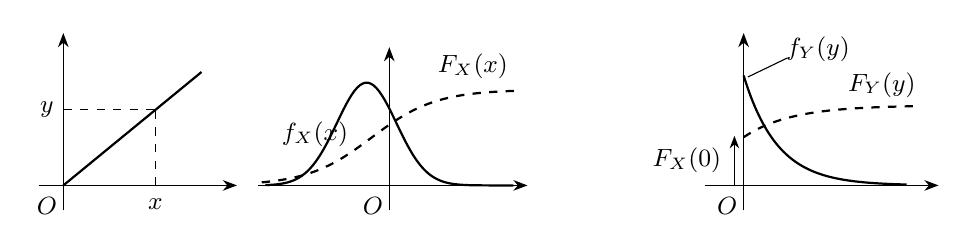
\begin{tikzpicture}[scale=0.9,every node/.style={font=\small}]

    % ---------------- (a) y = g(x) ----------------
    \begin{scope}
      \draw[-{Stealth[length=1.8mm]}] (-0.35,0) -- (2.45,0);
      \draw[-{Stealth[length=1.8mm]}] (0,-0.35) -- (0,2.15);
      \draw[thick] (0,0) -- (1.95,1.60);
      \draw[dashed] (1.30,0) -- (1.30,1.07);
      \draw[dashed] (0,1.07) -- (1.30,1.07);
      \node[left] at (0,1.07) {$y$};
      \node[below] at (1.30,-0.05) {$x$};
      \node[below left] at (0.05,-0.03) {$O$};
    \end{scope}

    % ---------------- (b) f_X(x) 与 F_X(x) ----------------
    \begin{scope}[xshift=4.6cm]
      \draw[-{Stealth[length=1.8mm]}] (-1.85,0) -- (1.95,0);
      \draw[-{Stealth[length=1.8mm]}] (0,-0.35) -- (0,1.95);
      \draw[thick] plot[domain=-1.75:1.75,samples=90]
        (\x,{1.45*exp(-(\x+0.32)^2/(2*0.42^2))});
      \draw[dashed,thick] plot[domain=-1.80:1.80,samples=90]
        (\x,{1.35/(1+exp(-2.2*\x-0.55))});
      \node at (-1.05,0.72) {$f_X(x)$};
      \node at (1.18,1.68) {$F_X(x)$};
      \node[below left] at (0.05,-0.03) {$O$};
    \end{scope}

    % ---------------- (c) f_Y(y) 与 F_Y(y) ----------------
    \begin{scope}[xshift=9.6cm]
      \draw[-{Stealth[length=1.8mm]}] (-0.55,0) -- (2.75,0);
      \draw[-{Stealth[length=1.8mm]}] (0,-0.35) -- (0,2.15);
      % f_X(0) 处（即 F_Y 的跳跃幅度）的竖直标线
      \draw[-{Stealth[length=1.6mm]}] (-0.13,0) -- (-0.13,0.70);
      \node[left] at (-0.18,0.35) {$F_X(0)$};
      % f_Y(y) = f_X(y)u(y)
      \draw[thick] plot[domain=0.0:2.3,samples=90]
        (\x,{1.55*exp(-2.1*\x)});
      \draw (0.06,1.53) -- (0.62,1.80);
      \node at (1.05,1.92) {$f_Y(y)$};
      % F_Y(y) = F_X(y)u(y)
      \draw[dashed,thick] plot[domain=0.0:2.4,samples=90]
        (\x,{0.68+0.45*(1-exp(-1.5*\x))});
      \node at (1.95,1.42) {$F_Y(y)$};
      \node[below left] at (0.05,-0.03) {$O$};
    \end{scope}

  \end{tikzpicture}

  \vspace{2pt}
  \captionof{figure}{半波整流图}\label{fig:1.9}
\end{center}

% EQNUMBERS: 1.18, 1.19, 1.20, 1.21, 1.22, 1.23, 1.24, 1.25, 1.26
% 原书编号连续，无跳号。

% =====================================================================
%  frag_D.tex  —— 《随机信号分析（第5版）》书 p.13 – p.15
%  内容：例1.10 续解 → 定理1.1 → 例1.11 → 1.3.2 二元函数 → 例1.12
%        → (1.33)–(1.39) → 例1.13 → 例1.14 → 1.3.3 瑞利与莱斯分布 → 例1.15
%  前一片段负责到书 p.12（例1.10 的题面与图1.9 在 p.12）。
% =====================================================================

\textbf{解}\quad 由已知
\[
Y=g(X)=\begin{cases}
X, & X\geqslant 0\\
0, & X<0
\end{cases}
\]
于是可得\nobreak：

\begin{citemize}
  \item ① 如果 $y<0$\nobreak，由于始终有 $Y\geqslant 0$\nobreak，因此事件 $\{Y\leqslant y\}$ 是不可能事件\nobreak，所以
  \[
  F_Y(y)=P[Y\leqslant y]=P[\varnothing]=0
  \]

  \item ② 如果 $y\geqslant 0$\nobreak，事件 $\{Y\leqslant y\}$ 等同于事件 $\{X\leqslant y\}$\nobreak，于是
  \[
  F_Y(y)=P[Y\leqslant y]=P[X\leqslant y]=F_X(y)
  \]
\end{citemize}

注意到 $F_Y(y)$ 在 $y=0$ 处有一个跳跃型间断点\nobreak，跳跃幅度为 $F_X(0)$\nobreak。因此
\begin{equation}
\begin{cases}
F_Y(y)=F_X(y)u(y)\\[2pt]
f_Y(y)=f_X(y)u(y)+F_X(0)\delta(y)
\end{cases}
\label{eq:1.27}
\end{equation}
\end{examplebox}

对于连续型随机变量\nobreak，如果 $g(x)$ 是单调递增或单调递减函数\nobreak，则有下面的定理\nobreak。

\bhead{定理1.1}\quad 设 $Y=g(X)$\nobreak，若 $g(x)$ 处处可导且恒有 $g'(x)>0$ 或 $g'(x)<0$\nobreak，则
\begin{equation}
f_Y(y)=\begin{cases}
f_X\bigl[h(y)\bigr]\bigl\lvert h'(y)\bigr\rvert, & a<y<b\\[2pt]
0, & \text{其他}
\end{cases}
\label{eq:1.28}
\end{equation}
式中\nobreak，$a=\min\bigl\{g(-\infty),g(+\infty)\bigr\}$\nobreak，$b=\max\bigl\{g(-\infty),g(+\infty)\bigr\}$\nobreak，$h(y)$ 是 $g(x)$ 的反函数\nobreak。

\begin{examplebox}
\textbf{例1.11}\quad 求 $Y=aX+b$ 的密度函数\nobreak。

\textbf{解}\quad 由于函数符合定理的条件\nobreak，且反函数形式为 $x=(y-b)/a$\nobreak，导函数为 $1/a$\nobreak。于是
\begin{equation}
f_Y(y)=\frac{1}{\lvert a\rvert}f_X\left(\frac{y-b}{a}\right)
\label{eq:1.29}
\end{equation}
\end{examplebox}

\subsection{二元函数}

二元函数表示为 $Z=g(X,Y)$\nobreak，确定其函数分布的基本方法同样是从定义出发
\begin{equation}
\begin{aligned}
F_Z(z)&=P\bigl[g(X,Y)\leqslant z\bigr]=P\Bigl[(X,Y)\in\bigl\{(x,y):g(x,y)\leqslant z\bigr\}\Bigr]\\
&=\iint_{\{(x,y):\,g(x,y)\leqslant z\}}f_{XY}(x,y)\dif x\dif y
\end{aligned}
\label{eq:1.30}
\end{equation}

\begin{examplebox}
\textbf{例1.12}\quad 求 $U=\min(X,Y)$ 与 $V=\max(X,Y)$ 的分布函数\nobreak。

\textbf{解}\quad 按定义\qquad $F_U(u)=P\bigl[\min(X,Y)\leqslant u\bigr]=P\bigl[(X\leqslant u)\cup(Y\leqslant u)\bigr]$

由概率的基本性质\qquad $P(A\cup B)=P(A)+P(B)-P(A\cap B)$

有
\begin{equation}
F_U(u)=F_X(u)+F_Y(u)-F_{XY}(u,u)
\label{eq:1.31}
\end{equation}

仿此有
\begin{equation}
\begin{aligned}
F_V(v)&=P\bigl[\max(X,Y)\leqslant v\bigr]=P\bigl[(X\leqslant v)\cap(Y\leqslant v)\bigr]\\
&=P\bigl[X\leqslant v,Y\leqslant v\bigr]=F_{XY}(v,v)
\end{aligned}
\label{eq:1.32}
\end{equation}
\end{examplebox}

更一般的函数关系可以是如下的二元至二元的映射组
\begin{equation}
\begin{cases}
U=g_1(X,Y)\\
V=g_2(X,Y)
\end{cases}
\label{eq:1.33}
\end{equation}
仿照一元函数\nobreak，对于连续型随机变量\nobreak，可用下面的公式确定其联合密度函数
\begin{equation}
f_{UV}(u,v)=f_{XY}\bigl[h_1(u,v),h_2(u,v)\bigr]\lvert J\rvert
\label{eq:1.34}
\end{equation}
式中\nobreak，$h_1()$ 与 $h_2()$ 为反函数\nobreak，$J$ 为雅可比行列式（Jacobian\nobreak）\nobreak，即
\begin{equation}
\begin{cases}
x=h_1(u,v)\\
y=h_2(u,v)
\end{cases},\qquad
J=\begin{vmatrix}
\dfrac{\partial h_1}{\partial u} & \dfrac{\partial h_1}{\partial v}\\[10pt]
\dfrac{\partial h_2}{\partial u} & \dfrac{\partial h_2}{\partial v}
\end{vmatrix}
=\begin{vmatrix}
\dfrac{\partial g_1}{\partial x} & \dfrac{\partial g_1}{\partial y}\\[10pt]
\dfrac{\partial g_2}{\partial x} & \dfrac{\partial g_2}{\partial y}
\end{vmatrix}^{-1}\neq 0
\label{eq:1.35}
\end{equation}

\begin{examplebox}
\textbf{例1.13}\quad 求 $Z=X+Y$ 的密度函数\nobreak。

\textbf{解}\quad 为了利用公式（1.34\nobreak）\nobreak，必须建立相同维数的映射组\nobreak。因而\nobreak，我们定义辅助变量 $U=Y$\nobreak，则函数\nobreak、相应的反函数形式与雅可比行列式如下
\[
\begin{cases}
Z=X+Y\\
U=Y
\end{cases},\qquad
\begin{cases}
x=z-u\\
y=u
\end{cases},\qquad
J=\begin{vmatrix}
1 & -1\\
0 & 1
\end{vmatrix}=1
\]
于是
\[
f_{ZU}(z,u)=f_{XY}(z-u,u)\times 1
\]
对该联合密度函数积分可得
\begin{equation}
f_Z(z)=f_{X+Y}(z)=\int_{-\infty}^{+\infty}f_{XY}(z-u,u)\dif u
\label{eq:1.36}
\end{equation}
如果 $X$ 与 $Y$ 独立\nobreak，则 $f_{XY}(x,y)=f_X(x)f_Y(y)$\nobreak，于是
\begin{equation}
f_Z(z)=f_{X+Y}(z)=\int_{-\infty}^{+\infty}f_X(z-u)f_Y(u)\dif u=f_X(z)*f_Y(z)
\label{eq:1.37}
\end{equation}
\end{examplebox}

上式中“$*$”表示卷积运算\nobreak。可见\nobreak，独立随机变量和的概率密度函数等于各概率密度函数的卷积\nobreak。相仿地\nobreak，还可以求出下面的结果
\begin{equation}
f_{XY}(z)=\int_{-\infty}^{+\infty}\frac{1}{\lvert u\rvert}f_{XY}\left(\frac{z}{u},u\right)\dif u
\label{eq:1.38}
\end{equation}
\begin{equation}
f_{X/Y}(z)=\int_{-\infty}^{+\infty}\lvert u\rvert f_{XY}(zu,u)\dif u
\label{eq:1.39}
\end{equation}

\begin{examplebox}
\textbf{例1.14}\quad 假定电阻库中的电阻精度均为 $\pm 1\%$\nobreak，误差服从均匀分布\nobreak。某电路中需要 20~k$\Omega$ 电阻\nobreak，问\nobreak：

（1\nobreak）取一个标称 20~k$\Omega$ 的电阻\nobreak，其实际值在 20~k$\Omega\pm 100~\Omega$ 以内的概率是多少\nobreak？

（2\nobreak）取两个标称 10~k$\Omega$ 的电阻串联\nobreak，其实际值在 20~k$\Omega\pm 100~\Omega$ 以内的概率是多少\nobreak？

\textbf{解}\nobreak：（1\nobreak）精度为 $\pm 1\%$\nobreak、标称 20~k$\Omega$ 电阻的真实电阻值是随机的\nobreak，范围在 20~k$\Omega\pm 200~\Omega$ 内均匀分布\nobreak，显然\nobreak，一个标称 20~k$\Omega$ 的电阻的实际值在 20~k$\Omega\pm 100~\Omega$ 以内的概率是 0.5\nobreak。

（2\nobreak）同理\nobreak，精度为 $\pm 1\%$\nobreak、标称 10~k$\Omega$ 的真实电阻值是随机的\nobreak，服从 10~k$\Omega\pm 100~\Omega$ 上的均匀分布\nobreak。随机取两个这样的电阻 $R_1,R_2$\nobreak，可以认为彼此独立\nobreak，串联后的阻值 $R=R_1+R_2$\nobreak，其分布为
\[
f_R(r)=f_{R_1}(r_1)*f_{R_2}(r_2)
\]
由于相同矩形函数卷积结果为三角形函数\nobreak，如图~\ref{fig:1.10} 所示\nobreak。图中阴影部分为“落在 20~k$\Omega\pm 100~\Omega$ 以内的概率”\nobreak，易见\nobreak，它是 0.75\nobreak。

\begin{center}
  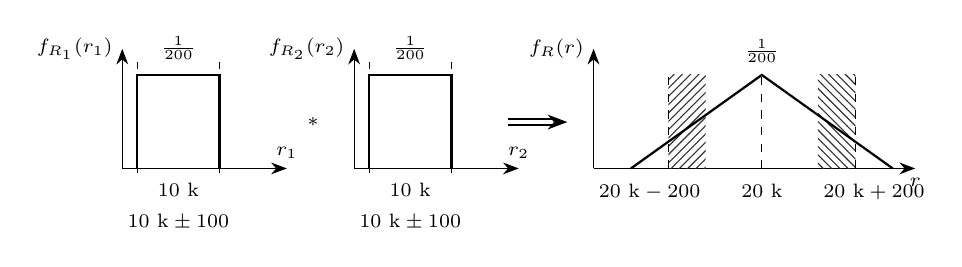
\begin{tikzpicture}[scale=0.95,every node/.style={font=\scriptsize}]
    % ---------------- (a) f_{R_1}(r_1) ----------------
    \begin{scope}
      \draw[-{Stealth[length=2mm]}] (-0.25,0) -- (1.95,0) node[above] {$r_1$};
      \draw[-{Stealth[length=2mm]}] (-0.25,0) -- (-0.25,1.60) node[left] {$f_{R_1}(r_1)$};
      \draw[thick] (-0.05,0) -- (-0.05,1.25) -- (1.05,1.25) -- (1.05,0);
      \draw[dashed] (-0.05,0) -- (-0.05,1.42);
      \draw[dashed] (1.05,0) -- (1.05,1.42);
      \node[anchor=south] at (0.50,1.32) {$\frac{1}{200}$};
      \draw (-0.05,0) -- (-0.05,-0.06);
      \draw (1.05,0) -- (1.05,-0.06);
      \node[below] at (0.50,-0.06) {$10~\text{k}$};
      \node[below] at (0.50,-0.48) {$10~\text{k}\pm 100$};
    \end{scope}
    % ---------------- 卷积号 ----------------
    \node at (2.30,0.62) {$*$};
    % ---------------- (b) f_{R_2}(r_2) ----------------
    \begin{scope}[xshift=3.10cm]
      \draw[-{Stealth[length=2mm]}] (-0.25,0) -- (1.95,0) node[above] {$r_2$};
      \draw[-{Stealth[length=2mm]}] (-0.25,0) -- (-0.25,1.60) node[left] {$f_{R_2}(r_2)$};
      \draw[thick] (-0.05,0) -- (-0.05,1.25) -- (1.05,1.25) -- (1.05,0);
      \draw[dashed] (-0.05,0) -- (-0.05,1.42);
      \draw[dashed] (1.05,0) -- (1.05,1.42);
      \node[anchor=south] at (0.50,1.32) {$\frac{1}{200}$};
      \draw (-0.05,0) -- (-0.05,-0.06);
      \draw (1.05,0) -- (1.05,-0.06);
      \node[below] at (0.50,-0.06) {$10~\text{k}$};
      \node[below] at (0.50,-0.48) {$10~\text{k}\pm 100$};
    \end{scope}
    % ---------------- 箭头 ----------------
    \draw[-{Stealth[length=2.5mm]},thick,double,double distance=1.6pt] (4.90,0.62) -- (5.70,0.62);
    % ---------------- (c) f_R(r) ----------------
    \begin{scope}[xshift=6.30cm]
      \draw[-{Stealth[length=2mm]}] (-0.25,0) -- (4.05,0) node[below] {$r$};
      \draw[-{Stealth[length=2mm]}] (-0.25,0) -- (-0.25,1.60) node[left] {$f_R(r)$};
      % 阴影：|r-20k| <= 100
      \fill[pattern=north east lines,pattern color=black!80]
        (0.75,0) -- (0.75,1.25) -- (1.25,1.25) -- (1.25,0) -- cycle;
      \fill[pattern=north west lines,pattern color=black!80]
        (2.75,0) -- (2.75,1.25) -- (3.25,1.25) -- (3.25,0) -- cycle;
      \draw[thick] (0.25,0) -- (2.00,1.25) -- (3.75,0);
      \draw[dashed] (2.00,0) -- (2.00,1.25);
      \draw[dashed] (0.75,0) -- (0.75,1.30);
      \draw[dashed] (3.25,0) -- (3.25,1.30);
      \node[anchor=south] at (2.00,1.28) {$\frac{1}{200}$};
      \node[below] at (0.50,-0.08) {$20~\text{k}-200$};
      \node[below] at (2.00,-0.08) {$20~\text{k}$};
      \node[below] at (3.50,-0.08) {$20~\text{k}+200$};
    \end{scope}
  \end{tikzpicture}
  \captionof{figure}{串联电阻的概率密度}\label{fig:1.10}
\end{center}

可见\nobreak，当误差服从均匀分布时\nobreak，由两个电阻串联的方法很可能获得更高精度的阻值\nobreak。
\end{examplebox}

\subsection{瑞利与莱斯分布}

理论分析与工程应用中经常遇到正态随机变量的变换\nobreak，这些变换衍生出一些重要的分布\nobreak。其中\nobreak，瑞利与莱斯分布是无线电技术与通信工程等领域的常见分布\nobreak。下面我们通过例子说明这两个分布\nobreak。

\begin{examplebox}
\textbf{例1.15}\quad 复随机变量 $Z=X+\ju Y=R\eu^{\ju\Theta}$\nobreak，其中实部与虚部是同分布的零均值正态随机变量\nobreak：$X\sim N(0,\sigma^2)$\nobreak，$Y\sim N(0,\sigma^2)$\nobreak，且 $X$ 与 $Y$ 独立\nobreak。讨论振幅 $R$ 与相位 $\Theta$ 的概率特性\nobreak。

\textbf{解}\nobreak：$R$\nobreak、$\Theta$ 与 $X$\nobreak、$Y$ 之间的函数\nobreak、反函数形式与雅可比行列式如下
\[
\begin{cases}
R=\sqrt{X^2+Y^2}\\
\Theta=\arctan(Y/X)
\end{cases},\quad
\begin{cases}
x=r\cos\theta\\
y=r\sin\theta
\end{cases},\quad
J=\begin{vmatrix}
\cos\theta & -r\sin\theta\\
\sin\theta & r\cos\theta
\end{vmatrix}=r
\]
根据 $X$ 与 $Y$ 独立\nobreak，有
\[
f_{XY}(x,y)=f_X(x)f_Y(y)=\frac{1}{2\pi\sigma^2}\eu^{-(x^2+y^2)/2\sigma^2}
\]
于是
\begin{equation}
\begin{aligned}
f_{R\Theta}(r,\theta)&=\begin{cases}
f_{XY}(r\cos\theta,r\sin\theta)r, & r\geqslant 0\\
0, & r<0
\end{cases}\\
&=\begin{cases}
\dfrac{r}{2\pi\sigma^2}\eu^{-r^2/2\sigma^2}, & r\geqslant 0\\[4pt]
0, & r<0
\end{cases}
\end{aligned}
\label{eq:1.40}
\end{equation}

边缘概率密度函数为
\begin{equation}
f_R(r)=\int_0^{2\pi}f_{R\Theta}(r,\theta)\dif\theta=\begin{cases}
\dfrac{r}{\sigma^2}\eu^{-r^2/2\sigma^2}, & r\geqslant 0\\[4pt]
0, & r<0
\end{cases}
\label{eq:1.41}
\end{equation}
\begin{equation}
f_\Theta(\theta)=\int_0^{+\infty}f_{R\Theta}(r,\theta)\dif r=\begin{cases}
\dfrac{1}{2\pi}, & \theta\in[0,2\pi)\\[4pt]
0, & \text{其他}
\end{cases}
\label{eq:1.42}
\end{equation}

式（1.41\nobreak）的分布被称为瑞利（Rayleigh\nobreak）分布\nobreak，如图~\ref{fig:1.11}(a) 所示\nobreak。由式（1.41\nobreak）易见\nobreak，$f_{R\Theta}(r,\theta)=f_R(r)/(2\pi)$\nobreak。注意到 $\int_{-\infty}^{\infty}f_R(r)\dif r=1$\nobreak，容易得出式（1.42\nobreak）\nobreak。

可见\nobreak，复变量 $Z$ 的幅度为瑞利分布\nobreak，相位为均匀分布\nobreak，并且 $f_{R\Theta}(r,\theta)=f_R(r)f_\Theta(\theta)$\nobreak，说明 $R$ 与 $\Theta$ 独立\nobreak。

进一步地\nobreak，如果 $X$ 与 $Y$ 的均值不为零\nobreak，分别为 $\mu_X$ 与 $\mu_Y$\nobreak，则
\[
f_{XY}(x,y)=f_X(x)f_Y(y)=\frac{1}{2\pi\sigma^2}\exp\left\{-\frac{(x-\mu_X)^2+(y-\mu_Y)^2}{2\sigma^2}\right\}
\]

\begin{center}
  \begin{tikzpicture}[scale=1.0,every node/.style={font=\scriptsize}]
    % ================= (a) 瑞利密度函数 =================
    \begin{scope}
      \draw[-{Stealth[length=2mm]}] (-0.20,0) -- (4.30,0) node[below] {$r$};
      \draw[-{Stealth[length=2mm]}] (-0.20,0) -- (-0.20,3.15) node[left] {$f_R(r)$};
      % 曲线 f_R(r)=r*exp(-r^2/2)
      \draw[thick] plot[domain=0:4.0,samples=120] (\x,{(\x)*exp(-(\x)*(\x)/2)});
      % 峰值虚线
      \draw[dashed] (1.0,0) -- (1.0,0.6065);
      \draw[dashed] (-0.55,0.6065) -- (1.0,0.6065);
      \draw (-0.20,0.6065) -- (0.06,0.6065);
      \draw (-0.20,1.20) -- (0.06,1.20);
      \node[left] at (-0.28,0.6065) {$0.61/\sigma$};
      \node[below] at (1.0,-0.06) {$\sigma$};
      \node[below left] at (0,0) {$O$};
    \end{scope}
    % ================= (b) 莱斯密度函数 =================
    \begin{scope}[xshift=5.00cm]
      \draw[-{Stealth[length=2mm]}] (-0.20,0) -- (4.30,0) node[below] {$r$};
      \draw[-{Stealth[length=2mm]}] (-0.20,0) -- (-0.20,3.15) node[left] {$f_R(r)$};
      % 莱斯密度曲线（示意形状，参数 mu_X=mu_Y=1.2, sigma=1）
      \draw[thick] plot[domain=0:4.0,samples=120]
        (\x,{(\x)*exp(-((\x)*(\x)+2.88)/2)*6.19});
      \draw (-0.20,0.6065) -- (0.06,0.6065);
      \draw (-0.20,1.20) -- (0.06,1.20);
      \node[below left] at (0,0) {$O$};
    \end{scope}
    % ================= 分图题 =================
    \node at (2.0,-0.95) {(a) 瑞利密度函数};
    \node at (7.0,-0.95) {(b) 莱斯密度函数};
  \end{tikzpicture}
  \captionof{figure}{瑞利与莱斯密度函数}\label{fig:1.11}
\end{center}

% =====================================================================
% EQNUMBERS: 1.27, 1.28, 1.29, 1.30, 1.31, 1.32, 1.33, 1.34, 1.35,
%            1.36, 1.37, 1.38, 1.39, 1.40, 1.41, 1.42
% 连续、无跳号。下一号应为 (1.43)（书 p.16，属下一片段）。
% 注意：书 p.15 末的 f_{XY}(x,y)（非零均值情形）原书未编号，(1.42) 之后
%       直接进入 p.16 的莱斯密度公式，推测该式为 (1.43)。
% =====================================================================

% =====================================================================
%  frag_E.tex  —— 《随机信号分析（第5版）》书 p.16 – p.18
%  内容：§1.3.3 瑞利与莱斯分布收尾（例1.15 续解 + 式(1.43)(1.44)）
%        → 1.4 数字特征与条件数学期望
%        → 1.4.1 数学期望（定义1.1，(1.45)(1.46)）
%        → 数学期望的基本性质与函数均值公式 (1.47)(1.48)
%        → 1.4.2 矩与联合矩（(1.49)）
%        → 1.4.3 无关与正交 + 图1.12 + 例1.16（(1.50)，其解续至书 p.19）
%  上一片段 frag_D 负责到书 p.15（含图1.11）；下一片段负责书 p.19 起。
% =====================================================================

% 【框的分界说明】原书书 p.15 底 – p.16 顶 属同一个灰底例题框（例1.15），
%   frag_D 已在图1.11 之前用 \end{examplebox} 收尾，故此处重新开框，以保证本
%   片段可独立编译。合并定稿时若要让例1.15 的灰底框跨页连续，可删去 frag_D 中
%   图1.11 之前的 \end{examplebox} 与下面这一行 \begin{examplebox}，并把图1.11
%   改为框内的 \captionof{figure}（与 frag_C 中图1.9 的做法相同）。
令
\[
\begin{cases}
a=\sqrt{\mu_X^2+\mu_Y^2}\\
\phi=\arctan(\mu_Y/\mu_X)
\end{cases},\qquad
\begin{cases}
\mu_X=a\cos\phi\\
\mu_Y=a\sin\phi
\end{cases}
\]
$f_{XY}(x,y)$ 的指数部分中
\[
\begin{aligned}
(x-\mu_X)^2+(y-\mu_Y)^2&=x^2+y^2+\mu_X^2+\mu_Y^2-2(x\mu_X+y\mu_Y)\\
&=r^2+a^2-2ra\cos(\theta-\phi)
\end{aligned}
\]
于是
\[
f_{R\Theta}(r,\theta)=\frac{r}{2\pi\sigma^2}\exp\left\{-\frac{r^2+a^2}{2\sigma^2}+\frac{ra\cos(\theta-\phi)}{\sigma^2}\right\}
\]
所以
\begin{equation}
\begin{aligned}
f_R(r)&=\int_0^{2\pi}f_{R\Theta}(r,\theta)\dif\theta
       =\frac{r\eu^{-(r^2+a^2)/2\sigma^2}}{2\pi\sigma^2}\int_0^{2\pi}\eu^{ra\cos(\theta-\phi)/\sigma^2}\dif\theta\\
&=\frac{r\eu^{-(r^2+a^2)/2\sigma^2}}{\sigma^2}I_0\left(\frac{ra}{\sigma^2}\right)\qquad(r\geqslant 0)
\end{aligned}
\label{eq:1.43}
\end{equation}
式中\nobreak，修正零阶贝塞尔函数
\begin{equation}
I_0(x)=\frac{1}{2\pi}\int_0^{2\pi}\eu^{x\cos\theta}\dif\theta
\label{eq:1.44}
\end{equation}
式（1.43\nobreak）的分布称为莱斯（Rician\nobreak）分布（或称广义瑞利分布\nobreak）\nobreak，如图 1.11(b)所示\nobreak。若有必要\nobreak，还可以进一步求出 $f_\Theta(\theta)$\nobreak，并可发现 $R$ 与 $\Theta$ 一般不独立\nobreak。
\end{examplebox}

在电子与通信工程等应用中\nobreak，信号与噪声在许多时候服从高斯分布\nobreak。分析中常常要讨论这些信号或噪声的两个正交分量及其幅度与相位的特性\nobreak，它们在数学上分别对应于复变量的实部\nobreak、虚部\nobreak、振幅与相位\nobreak，因此\nobreak，将大量地用到瑞利与莱斯分布\nobreak。

\section{数字特征与条件数学期望}

随机变量的一些重要特征可用少量的数值来刻画\nobreak，这些数值是一些统计平均值\nobreak，通称为随机变量或分布函数的数字特征\nobreak。

\subsection{数学期望（或统计平均\nobreak）}

\thm{定义1.1} 若随机变量 $X$ 的密度函数为 $f(x)$\nobreak，且 $\int_{-\infty}^{+\infty}\lvert x\rvert f(x)\dif x<+\infty$\nobreak，则
\begin{equation}
\E(X)=\int_{-\infty}^{+\infty}xf(x)\dif x
\label{eq:1.45}
\end{equation}
称为 $X$ 的数学期望（Expectation\nobreak）\nobreak，或统计（集\nobreak）平均（Ensemble Average\nobreak）\nobreak。

定义中的条件 $\int_{-\infty}^{+\infty}\lvert x\rvert f(x)\dif x<+\infty$ 是为了保证 $\E(X)$ 存在\nobreak。式（1.45\nobreak）中可能涉及冲激函数 $\delta(x)$\nobreak。特别是\nobreak，当 $X$ 为离散型时\nobreak，$f(x)$ 完全由冲激函数组成\nobreak，由于冲激函数的筛选性质使得 $\int_{-\infty}^{+\infty}xp_i\delta(x-x_i)\dif x=x_ip_i$\nobreak，因此
\begin{equation}
\E(X)=\sum_i x_ip_i
\label{eq:1.46}
\end{equation}
数学期望刻画了 $f(x)$ 的中心位置\nobreak，其物理意义是 $X$ 取值的算术平均
\[
\overline{X}=(X_1+\cdots+X_N)/N
\]
$\E[X]$ 也常称为均值（Mean\nobreak）\nobreak，并简记为 $m_X$\nobreak。各种典型分布及其均值将在 1.6 节中讨论\nobreak。

数学期望的基本性质有\nobreak：

\begin{citemize}
  \item ① 线性\nobreak：$\E(aX+bY+c)=a\E(X)+b\E(Y)+c$\nobreak，其中\nobreak，$a,b,c$ 为任意常数\nobreak。
  \item ② 若 $X_1,X_2,\cdots,X_n$ 独立\nobreak，则 $\E(X_1\cdots X_n)=\E(X_1)\E(X_2)\cdots\E(X_n)$\nobreak。
\end{citemize}

而且可以证明\nobreak，随机变量的函数的均值可直接计算\nobreak。例如\nobreak，对于 $Z=g(X)$\nobreak，有
\begin{equation}
\E[g(X)]=\E[Z]=\int_{-\infty}^{+\infty}zf_Z(z)\dif z=\int_{-\infty}^{+\infty}g(x)f_X(x)\dif x
\label{eq:1.47}
\end{equation}
又例如\nobreak，$Z=g(X_1,X_2,\cdots,X_n)$\nobreak，则
% 【排版说明】原书 (1.48) 此处为两行；按本书版心（132mm / 11pt）照排会超宽
%   约 53pt，故把第二个等号后的被积函数再折一行（内容一字未改）。
\begin{equation}
\begin{aligned}
\E[g(X_1,X_2,\cdots,X_n)]&=\E[Z]=\int_{-\infty}^{+\infty}zf_Z(z)\dif z\\
&=\int_{-\infty}^{+\infty}\cdots\int_{-\infty}^{+\infty}g(x_1,x_2,\cdots,x_n)\\
&\qquad\times f_{X_1\cdots X_n}(x_1,x_2,\cdots,x_n)\dif x_1\cdots\dif x_n
\end{aligned}
\label{eq:1.48}
\end{equation}
采用直接计算公式避免了求解函数随机变量的密度函数\nobreak，使得计算简便\nobreak。

数学上\nobreak，数学期望还常常采用更为简洁的书写方式\nobreak，如 $EX$\nobreak，$EX^2$\nobreak，$Eg(X)$ 等\nobreak，应注意识别\nobreak。

\subsection{矩与联合矩}

基于数学期望\nobreak，可定义单个或多个随机变量的一批数字特征\nobreak，统称为 $k$ 阶矩（Moment\nobreak）与 $(k+r)$ 阶联合矩（或混合矩\nobreak）（Joint Moment\nobreak）\nobreak。
\[
\begin{array}{lll}
\text{绝对原点矩\nobreak：} & \E\bigl(\lvert X\rvert^k\bigr) & \E\bigl(\lvert X\rvert^k\lvert Y\rvert^r\bigr)\\[4pt]
\text{原点矩\nobreak：} & m_k=\E\bigl(X^k\bigr) & m_{k+r}=\E\bigl(X^kY^r\bigr)\\[4pt]
\text{中心矩\nobreak：} & \mu_k=\E\bigl(X-EX\bigr)^k & \mu_{k+r}=\E\bigl[(X-EX)^k(Y-EY)^r\bigr]
\end{array}
\]
如果令 $X-EX$ 是 $X$ 的中心化随机变量\nobreak，则中心矩是中心化随机变量的普通原点矩\nobreak，因此它与原点矩有许多相同的特征\nobreak。

矩与联合矩中\nobreak，特别重要的有\nobreak：

（1\nobreak）均方差
\[
m_2=EX^2
\]
（2\nobreak）方差
\[
\mu_2=\E(X-EX)^2
\]
方差（Variance\nobreak）常记为 $\sigma^2$\nobreak、$\Var(X)$ 或 $D(X)$\nobreak。并称 $\sigma=\sqrt{\Var(X)}$ 为标准差（Standard Deviation\nobreak）\nobreak，它刻画出 $X$ 围绕 $EX$ 的散布程度\nobreak。例如\nobreak，正态随机变量落入 $EX$ 的 $\pm3\sigma$ 邻域内的概率达 99.97\%\nobreak。方差的基本性质有\nobreak：
% 原书此行版式为「① 公式…；   (1.49)」——左侧 ①、公式居中、编号右对齐，故用 flalign。
\begin{flalign}
\text{①}\quad & \Var(X)=EX^2-(EX)^2\text{\nobreak；} & \label{eq:1.49}
\end{flalign}
② $\Var(aX+c)=a^2\Var(X)$\nobreak，$a,c$ 为任意常数\nobreak；

③ 如果 $X_i,i=1,\cdots,n$\nobreak，两两独立\nobreak，则
\[
\Var(X_1+X_2+\cdots+X_n)=\Var(X_1)+\Var(X_2)+\cdots+\Var(X_n)
\]
（3\nobreak）联合矩
\[
m_{11}=\E(XY)
\]
（4\nobreak）协方差
\[
\mu_{11}=\E\bigl[(X-EX)(Y-EY)\bigr]
\]
协方差（Covariance\nobreak）常记为 $\Cov(X,Y)$\nobreak，其基本性质有\nobreak：
\begin{flalign}
\text{①}\quad & \Cov(X,Y)=\E(XY)-(\E X)(\E Y) & \label{eq:1.50}
\end{flalign}
② $\Cov(X+Y,Z)=\Cov(X,Z)+\Cov(Y,Z)$

（5\nobreak）相关系数
\[
\rho_{XY}=\frac{\Cov(X,Y)}{\sigma_X\sigma_Y}
\]
相关系数是归一化随机变量的协方差\nobreak，有 $\lvert\rho_{XY}\rvert\leqslant 1$\nobreak。并且称
\[
\rho=\begin{cases}
0, & X\text{与}Y\text{无关}\\
\pm 1, & X\text{与}Y\text{线性（正或负\nobreak）相关}
\end{cases}
\]

\subsection{无关与正交}

$\E(XY)$\nobreak，$\Cov(X,Y)$ 与 $\rho_{XY}$ 常用于刻画随机变量之间的关联程度\nobreak。尤其是 $\rho_{XY}$ 提供了一种归一化的测度\nobreak。定义\nobreak：

① 随机变量 $X$ 与 $Y$ 无关（Uncorrelated\nobreak）\nobreak：$\Cov(X,Y)=0$ 或 $\rho_{XY}=0$\nobreak，也就是\nobreak，$\E(XY)=(\E X)(\E Y)$\nobreak。

② 随机变量 $X$ 与 $Y$ 正交（Orthogonal\nobreak）\nobreak：$\E(XY)=0$\nobreak。

显然\nobreak，如果 $EX$ 与 $EY$ 中至少有一个为 0 时\nobreak，则正交与无关等价\nobreak。正交与无关是基于二阶矩的概念\nobreak，而独立性是基于概率特性的概念\nobreak，两者的出发角度不一样\nobreak。一般而言\nobreak，独立比无关更为苛刻\nobreak，但对正态随机变量\nobreak，两者是等同的\nobreak。独立\nobreak、无关与正交三者的关系如图 1.12 所示\nobreak。

\begin{figure}[htbp]
  \centering
  \begin{tikzpicture}[every node/.style={font=\small}]
    % ---------------- 三个椭圆 ----------------
    \node (ind) at (0,0) {独立};
    \draw (ind) ellipse [x radius=0.82cm,y radius=0.50cm];
    \node (unc) at (3.50,0) {无关};
    \draw (unc) ellipse [x radius=0.82cm,y radius=0.50cm];
    \node (ort) at (8.10,0) {正交};
    \draw (ort) ellipse [x radius=0.82cm,y radius=0.50cm];

    % ---------------- 独立 ←→ 无关：两条平行单箭头，注「如果正态」 ----------------
    \draw[-{Stealth[length=2mm]}] (0.95,0.18) -- (2.55,0.18);
    \draw[-{Stealth[length=2mm]}] (2.55,-0.18) -- (0.95,-0.18);
    \node[below] at (1.75,-0.26) {如果正态};

    % ---------------- 无关 ←→ 正交：一条双向箭头，注「EX 与 EY 至少一个为 0」 ----------------
    \draw[{Stealth[length=2mm]}-{Stealth[length=2mm]}] (4.45,0.14) -- (7.15,0.14);
    \node[below,align=center] at (5.80,-0.20) {$EX$ 与 $EY$ 至少\\一个为 0};
  \end{tikzpicture}
  \caption{独立\nobreak、无关与正交的关系}
  \label{fig:1.12}
\end{figure}

% 【框的分界说明】原书灰底例题框（例1.16）在此处**并未结束**，其解答继续到
%   书 p.19 顶部（“$D(Y)=2/3$、而由 $D$ 区域的对称性可得 $E(XY)=\cdots=0$、
%   可见，$X$ 与 $Y$ 虽不独立（由例1.9），但相互无关且正交。”）。
%   本框跨页延续到书 p.19，由 frag_F 首行 \end{examplebox} 收尾。
\begin{examplebox}
\textbf{例1.16}\quad 二维均匀分布为
\[
f(x,y)=\begin{cases}
1/4, & 0\leqslant x\leqslant 2,\ \lvert y\rvert\leqslant 2-x\\
0, & \text{其他}
\end{cases}
\]
讨论 $X$ 与 $Y$ 的基本数字特征\nobreak。

\textbf{解}\nobreak：利用例 1.6 的结果
\[
f_X(x)=\begin{cases}
1-x/2, & x\in[0,2]\\
0, & \text{其他}
\end{cases}
\]
\[
\E(X)=\int_0^2 x\left(1-\frac{1}{2}x\right)\dif x
     =\left.\left(\frac{1}{2}x^2-\frac{1}{6}x^3\right)\right|_0^2=\frac{2}{3}
\]
\[
\E(X^2)=\int_0^2 x^2\left(1-\frac{1}{2}x\right)\dif x
       =\left.\left(\frac{1}{3}x^3-\frac{1}{8}x^4\right)\right|_0^2=\frac{2}{3}
\]
\[
D(X)=EX^2-(EX)^2=\frac{2}{3}-\left(\frac{2}{3}\right)^2=\frac{2}{9}
\]
同理可得
\[
\E(Y)=\int_{-2}^{2}yf_Y(y)\dif y=0
\]
\[
\begin{aligned}
\E(Y^2)&=\int_{-2}^{2}y^2f_Y(y)\dif y
        =\int_{-2}^{0}y^2\frac{2+y}{4}\dif y+\int_0^2 y^2\frac{2-y}{4}\dif y\\
&=2\int_0^2\left(\frac{1}{2}y^2-\frac{1}{4}y^3\right)\dif y
  =\left.\left(\frac{1}{3}y^3-\frac{1}{8}y^4\right)\right|_0^2=\frac{2}{3}
\end{aligned}
\]

% =====================================================================
% EQNUMBERS: 1.43, 1.44, 1.45, 1.46, 1.47, 1.48, 1.49, 1.50
% 连续、无跳号，与扫描件锚点一致：
%   书 p.16: (1.43) (1.44) (1.45) (1.46)
%   书 p.17: (1.47) (1.48) (1.49)
%   书 p.18: (1.50)
% 图号：图1.12（本片段唯一插图；图1.11 由 frag_D 产出）。
% 下一号应为 (1.51)（书 p.19）。
% =====================================================================

% =====================================================================
%  frag_F.tex  —— 《随机信号分析（第5版）》书 p.19 – p.21
%  内容：例1.16 灰底框收尾（书 p.19 顶）→ 1.4.4 条件数学期望 → (1.51)–(1.56)
%        → 例1.17（灰底框，跨书 p.19–p.20）→ 例1.18 → 例1.19（灰底框，跨 p.20–p.21）
%        → 1.4.5 重要不等式 → 定理1.2 (1.57) → 定理1.3 (1.58)
%        → 1.5 特征函数 → 1.5.1 （一维）特征函数 → 1. 基本概念 → 定义1.2 (1.59)
%  编号：第一个编号公式 (1.51)，最后一个 (1.59)，连续、无跳号。
%  图/表：本片段无插图、无表格。
% =====================================================================

% ---------------------------------------------------------------------
% 【跨页灰底框 · 入口】书 p.18 的「例1.16 二维均匀分布」灰底例题框一直延续到
% 书 p.19 顶部（书 p.19 的第一行仍在该框内），故本片段第一行先补 \end{examplebox}，
% 用以与 frag_E.tex（书 p.16–p.18）末尾未闭合的 \begin{examplebox} 配对。
% 若最终 assemble 时确认 frag_E.tex 已自行闭合该框，请删除下面这一行。
% ---------------------------------------------------------------------
\end{examplebox}

\[
D(Y)=2/3
\]

而由 $D$ 区域的对称性可得
\[
E(XY)=\int_{-\infty}^{+\infty}\!\!\int_{-\infty}^{+\infty}xyf(x,y)\dif x\dif y
=\iint\limits_D \frac{1}{4}xy\dif x\dif y=0
\]
可见\nobreak，$X$ 与 $Y$ 虽不独立（由例1.9\nobreak）\nobreak，但相互无关且正交\nobreak。

\subsection{条件数学期望}

在一定条件下的数学期望\nobreak，称为条件数学期望（或条件均值\nobreak）\nobreak。以二维为例\nobreak，定义如下\nobreak：
\begin{equation}
E(X|Y=y)=\int_{-\infty}^{+\infty}xf_{X|Y}(x|y)\dif x
=\frac{\int_{-\infty}^{+\infty}xf_{XY}(x,y)\dif x}{f_Y(y)}
\label{eq:1.51}
\end{equation}
对于离散型随机变量\nobreak，显然
\begin{equation}
E(X|Y=y_j)=\frac{\sum\limits_i x_ip_{ij}}{p_j}
\label{eq:1.52}
\end{equation}
容易看出\nobreak，$E(X|Y=y)$ 是 $y$ 的函数\nobreak，有时也简记为 $E(X|y)$\nobreak。如果该函数的自变量为随机变量 $Y$\nobreak，则 $E(X|Y)$ 是随机变量的函数\nobreak，因此是一个新的随机变量\nobreak。进一步对它求平均有
% 说明：原书式(1.53)排成一行。本重排版心 132mm、11pt 字号，一行放不下（式号会被
%   挤到次行），故按原书 "=" 处折成两行，内容完全相同。
\begin{equation}
\begin{split}
E[E(X|Y)]&=\int_{-\infty}^{+\infty}E(X|y)f_Y(y)\dif y\\
&=\int_{-\infty}^{+\infty}\!\!\int_{-\infty}^{+\infty}xf_{XY}(x,y)\dif x\dif y=E(X)
\end{split}
\label{eq:1.53}
\end{equation}
该式称为全期望公式\nobreak。

条件期望与一般期望有相似的基本性质\nobreak，并有如下一些新性质\nobreak：

% 说明：原书此处 ①②③ 三个条目均从版心左端起排（非悬挂缩进），公式另起居中。
\begin{citemize}
  \item ① $E(aX+bY+c|Z)=aE(X|Z)+bE(Y|Z)+c$\nobreak，$a,b,c$ 为任意常数\nobreak。

  可见\nobreak，条件期望也是线性的\nobreak。

  \item ② 如果 $X$ 与 $Y$ 独立\nobreak，则
  \begin{equation}
  E(X|Y)=E(X)
  \label{eq:1.54}
  \end{equation}
  更为一般地\nobreak，
  \begin{equation}
  E\{g(X,Y)|Y=y\}=E\{g(X,y)\}
  \label{eq:1.55}
  \end{equation}
  可见\nobreak，独立的随机变量为条件时\nobreak，条件不起作用\nobreak。

  \item ③
  \begin{equation}
  E[h(Y)g(X)|Y]=h(Y)E[g(X)|Y]
  \label{eq:1.56}
  \end{equation}
  可见\nobreak，对于条件期望\nobreak，给定的条件部分等同于确知量\nobreak。
\end{citemize}

% ---------------------------------------------------------------------
% 【跨页灰底框】例1.17 的灰底框自书 p.19 下端起，延续到书 p.20 上部；
% 本片段（p.19–p.21）整体包含该框，故此处正常 \begin{examplebox}。
% ---------------------------------------------------------------------
\begin{examplebox}
\textbf{例1.17}\quad 证明条件期望的上述基本性质①与②\nobreak。

\textbf{证明\nobreak：}（1\nobreak）先考虑 $Z=z$ 条件下的情况
\[
\begin{aligned}
E(aX+bY+c|Z=z)&=\int_{-\infty}^{+\infty}\!\!\int_{-\infty}^{+\infty}
  (ax+by+c)f_{XY|Z}(x,y|Z=z)\dif x\dif y\\
&=a\int_{-\infty}^{+\infty}\!\!\int_{-\infty}^{+\infty}xf_{XY|Z}(x,y|Z=z)\dif x\dif y\,+\\
&\qquad b\int_{-\infty}^{+\infty}\!\!\int_{-\infty}^{+\infty}yf_{XY|Z}(x,y|Z=z)\dif x\dif y\,+\\
&\qquad c\int_{-\infty}^{+\infty}\!\!\int_{-\infty}^{+\infty}f_{XY|Z}(x,y|Z=z)\dif x\dif y
\end{aligned}
\]
由于 $f_{XY|Z}(x,y|Z=z)=\dfrac{f_{XYZ}(x,y,z)}{f_Z(z)}$\nobreak，因此

% ===================== 以下为书 p.20 =====================
\[
\begin{aligned}
\int_{-\infty}^{+\infty}\!\!\int_{-\infty}^{+\infty}xf_{XY|Z}(x,y|Z=z)\dif x\dif y
&=\int_{-\infty}^{+\infty}x\,\frac{\int_{-\infty}^{+\infty}f_{XYZ}(x,y,z)\dif y}{f_Z(z)}\dif x\\
&=\int_{-\infty}^{+\infty}x\,\frac{f_{XZ}(x,z)}{f_Z(z)}\dif x=E(X|Z=z)
\end{aligned}
\]
同理
\[
\int_{-\infty}^{+\infty}\!\!\int_{-\infty}^{+\infty}yf_{XY|Z}(x,y|Z=z)\dif x\dif y=E(Y|Z=z)
\]
\[
\int_{-\infty}^{+\infty}\!\!\int_{-\infty}^{+\infty}f_{XY|Z}(x,y|Z=z)\dif x\dif y=1
\]
所以
\[
E(aX+bY+c|Z=z)=aE(X|Z=z)+bE(Y|Z=z)+c
\]
再将条件 $Z=z$ 更换为随机变量 $Z$\nobreak，得到该性质\nobreak。

（2\nobreak）如果 $X$ 与 $Y$ 独立\nobreak，则 $f_{XY}(x,y)=f_X(x)f_Y(y)$\nobreak，于是
\[
E(X|Y=y)=\int_{-\infty}^{+\infty}x\,\frac{f_{XY}(x,y)}{f_Y(y)}\dif x
=\int_{-\infty}^{+\infty}xf_X(x)\dif x=E(X)
\]
将条件 $Y=y$ 更换为随机变量 $Y$\nobreak，得到该性质\nobreak。或者
\[
\begin{aligned}
E\{g(X,Y)|Y=y\}&=\int_{-\infty}^{+\infty}g(x,y)\frac{f_{XY}(x,y)}{f_Y(y)}\dif x\\
&=\int_{-\infty}^{+\infty}g(x,y)f_X(x)\dif x=E\{g(X,y)\}
\end{aligned}
\]
\end{examplebox}

\begin{examplebox}
\textbf{例1.18}\quad 二维均匀分布
\[
f(x,y)=\begin{cases}
1/4, & 0\leqslant x\leqslant 2,\ \lvert y\rvert\leqslant 2-x\\
0, & \text{其他}
\end{cases}
\]
如例1.9所述\nobreak，求\nobreak：

（1\nobreak）$E(X|Y=0)$ 与 $E(X|Y=1)$\nobreak；\qquad （2\nobreak）$E(X|Y)$ 及其取值范围\nobreak。

\textbf{解\nobreak：}（1\nobreak）根据例1.9的 $f(x|y)$ 结果\nobreak，条件事件 $(X|Y=0)$ 与 $(X|Y=1)$ 分别服从均匀分布 $U(0,2)$ 与 $U(0,1)$\nobreak，于是
\[
E(X|Y=0)=1\qquad E(X|Y=1)=1/2
\]
（2\nobreak）如果考虑随机变量 $Y\in[-2,2]$\nobreak，则条件事件 $(X|Y)$ 服从均匀分布 $U(0,2-\lvert Y\rvert)$\nobreak，于是
\[
E(X|Y)=(2-\lvert Y\rvert)/2=1-\lvert Y\rvert/2
\]
易见\nobreak，它是一个随机变量\nobreak，由 $Y$ 的取值范围可知其取值范围为 $[0,1]$\nobreak。
\end{examplebox}

% ---------------------------------------------------------------------
% 【跨页灰底框】例1.19 的灰底框自书 p.20 下端起，延续到书 p.21 上部，
% 本片段整体包含该框（在书 p.21 的 $E(Y)=500$ 元一行之后闭合）。
% ---------------------------------------------------------------------
\begin{examplebox}
\textbf{例1.19}\quad 某小店平均每天有 50 名顾客\nobreak，每人平均购买 10 元的商品\nobreak。问小店每天的平均营业额是多少\nobreak？

\textbf{解\nobreak：}由常识可知\nobreak，平均营业额 $=50\times10=500$ 元\nobreak。而其严格的数学分析如下\nobreak：令每天的顾客数为 $N$\nobreak，每人购买量为 $X_i$ 元\nobreak，$i=1,2,\cdots,N$\nobreak，这里 $X_i$ 与 $N$ 都是随机的\nobreak。可见\nobreak，营业额为 $Y=\sum\limits_{i=1}^{N}X_i$\nobreak，于是\nobreak，我们需要计算 $E(Y)$\nobreak。

然而\nobreak，$Y$ 由多个随机变量“合成”\nobreak，形如\nobreak，$Y=g(N,X_1,X_2,\cdots,X_N)$\nobreak，但这里的合成关系不是一般的函数\nobreak，因此无法用前面的方法求解\nobreak。下面借助条件平均来求解\nobreak。首先\nobreak，假设条件 $N=n$\nobreak，有
\[
E(Y|N=n)=E\left(\sum_{i=1}^{n}X_i\Big|N=n\right)=\sum_{i=1}^{n}E(X_i|N=n)
\]

% ===================== 以下为书 p.21 =====================
可合理地认为 $N$ 与 $X_i$ 独立\nobreak，利用式(1.54)有\nobreak，$E(X_i|N=n)=E(X_i)$\nobreak，
\[
E(Y|N=n)=\sum_{i=1}^{n}E(X_i)=10n
\]
而 $E(Y|N)=10N$\nobreak，所以
\[
E(Y)=E\big[E(Y|N)\big]=E[10N]=10\times50=500\text{（元\nobreak）}
\]
\end{examplebox}

计算复杂问题的均值时\nobreak，利用条件数学期望实施“分步”计算常常是一种极为有效的方法\nobreak：选择某个变量为前提条件\nobreak，先计算条件均值\nobreak，再借助全期望公式计算总的均值\nobreak。

\subsection{重要不等式}

概率论中两个最为基本与重要的不等式如下\nobreak，它们在后面的分析与证明中经常用到\nobreak。

\thm{定理1.2}（切比雪夫不等式\nobreak）（Chebyshev Inequality\nobreak）\quad 设 $X$ 为任一具有有限方差的随机变量\nobreak，对任意 $\varepsilon>0$\nobreak，有
\begin{equation}
P\bigl\{\lvert X-EX\rvert\geqslant\varepsilon\bigr\}\leqslant\frac{\sigma_X^2}{\varepsilon^2}
\label{eq:1.57}
\end{equation}
从另一个方面看\nobreak，切比雪夫不等式指出\nobreak，$X$ 落在 $m=EX$ 的 $\varepsilon$ 邻域 $(m-\varepsilon,m+\varepsilon)$ 内的概率大于 $1-\dfrac{\sigma^2}{\varepsilon^2}$\nobreak。我们知道方差 $\sigma^2$ 是随机变量分散程度的度量\nobreak，只要方差非常小\nobreak，$X$ 集中在 $m$ 的附近的概率就非常高\nobreak。如果方差 $\sigma^2=0$\nobreak，则 $X$ 完全集中在 $m$ 一点上\nobreak。因为对于任意小的 $\varepsilon$\nobreak，$P\bigl\{\lvert X-m\rvert\geqslant\varepsilon\bigr\}=0$\nobreak，或者说\nobreak，$P\{X\in(m-\varepsilon,m+\varepsilon)\}=1$\nobreak，即 $P\{X=m\}=1$\nobreak，$X$ 以概率 1 取 $m$\nobreak。

切比雪夫不等式是通用的\nobreak，无须知道 $X$ 的具体分布\nobreak。例如
\[
P\bigl[\lvert X-m\rvert<3\sigma\bigr]>1-\frac{\sigma^2}{9\sigma^2}\approx88.89\%
\]
由于是通用的\nobreak，这个估计是“保守”的\nobreak。比如\nobreak，在正态分布的特定条件下\nobreak，可以准确算出\nobreak，上述概率值实际上高达 99.74\%\nobreak。

\thm{定理1.3}（柯西-施瓦兹不等式\nobreak）（Cauchy-Schwarz Inequality\nobreak）\quad 设 $X,Y$ 为任意两个随机变量\nobreak，若 $E\lvert X\rvert^2<+\infty$\nobreak，$E\lvert Y\rvert^2<+\infty$\nobreak，则 $E(XY)$ 存在\nobreak，且
\begin{equation}
\lvert E(XY)\rvert^2\leqslant(E\lvert X\rvert^2)(E\lvert Y\rvert^2)
\label{eq:1.58}
\end{equation}

\section{特征函数}

特征函数是一种重要的数学工具\nobreak，它是随机变量概率密度函数的傅里叶变换\nobreak。在许多分析中\nobreak，使用它比使用分布与密度函数更加有效\nobreak。

\subsection{（一维\nobreak）特征函数}

\bhead{1.\ 基本概念}

\thm{定义1.2}\quad 随机变量 $X$ 的特征函数（Characteristic Function\nobreak）定义为
\begin{equation}
\phi_X(v)=E[\eu^{\ju vX}]
\label{eq:1.59}
\end{equation}
式中\nobreak，$\ju=\sqrt{-1}$\nobreak，$v$ 为确定的实变量\nobreak。

% =====================================================================
% EQNUMBERS: 1.51, 1.52, 1.53, 1.54, 1.55, 1.56, 1.57, 1.58, 1.59
% 连续、无跳号。上一号 (1.50) 在书 p.18（frag_E.tex）；下一号 (1.60)
% 在书 p.22（frag_G.tex）。
% 本片段无插图、无表格。
% =====================================================================

% =====================================================================
%  frag_G.tex  —— 《随机信号分析（第5版）》书 p.22 – p.24
%  内容：§1.5 特征函数（续）
%        p.22：(1.60) 连续/离散特征函数计算 → (1.61) 傅里叶变换对 →
%              定理1.4（密度函数与特征函数是一对傅里叶变换）→ 图1.13 →
%              定理1.5（唯一性定理）→ 2. 基本性质 → 性质1 → (1.62)
%        p.23：图1.14（独立随机变量之和）→ 性质2 → (1.63) →
%              例1.20（二项分布）→ 例1.21（指数分布）→ 例1.22（正态分布）
%        p.24：性质3 → (1.64) → 推论 → (1.65) → 例1.23（1~4 阶原点矩）→
%              §1.5.2 多维（联合）特征函数 → 1. 基本概念 → 定义1.3 → (1.66)
%              → 二维连续型联合特征函数（无编号，p.24 末；其离散型对应式
%                在书 p.25 页首，不属本片段）
%  编号：本片段第一个编号公式为 (1.60)。
%  图号：图1.13、图1.14。
% =====================================================================

根据均值的有关公式\nobreak，当 $X$ 为连续型或离散型随机变量时\nobreak，其特征函数可以分别计算如下
\begin{equation}
\phi_X(v)=\int_{-\infty}^{+\infty}\eu^{\ju vx}f_X(x)\dif x,\quad
\phi_X(v)=\sum_i \eu^{\ju vx_i}p_i
\label{eq:1.60}
\end{equation}

在信号与系统中我们知道\nobreak，时间信号 $f(t)$ 的傅里叶变换与反变换定义为
\begin{equation}
F(\ju\omega)=\int_{-\infty}^{+\infty}f(t)\eu^{-\ju\omega t}\dif t,\quad
f(t)=\frac{1}{2\pi}\int_{-\infty}^{+\infty}F(\ju\omega)\eu^{\ju\omega t}\dif\omega
\label{eq:1.61}
\end{equation}
简记为\nobreak：$f(t)\leftrightarrow F(\ju\omega)$\nobreak。其中\nobreak，$F(\ju\omega)$ 有时直接记为 $F(\omega)$\nobreak，它们是信号分析中的两种习惯记法\nobreak。本书主要采用带 $\ju$ 的 $F(\ju\omega)$ 形式标记信号的傅里叶变换与系统的频率响应\nobreak。

如果将式（1.60\nobreak）中的 $v$ 更换为 $-v$\nobreak，则
\[
\phi(-v)=\int_{-\infty}^{+\infty}f_X(x)\eu^{-\ju vx}\dif x
\]
该式的右边是傅里叶变换的标准形式\nobreak，记为 $f_X(x)\leftrightarrow\phi_X(-v)$\nobreak。由此可得下面的定理\nobreak。

\thm{定理1.4} 随机变量 $X$ 的密度函数 $f_X(x)$ 与其特征函数 $\phi_X(v)$ 是一对傅里叶变换\nobreak，即
\[
f_X(x)\leftrightarrow\phi_X(-v)\qquad\text{或}\qquad f_X(-x)\leftrightarrow\phi_X(v)
\]

定理 1.4 说明\nobreak，可以利用傅里叶变换计算特征函数\nobreak：先求密度函数的傅里叶变换\nobreak，而后将结果中的 $\omega$ 更换为 $-v$\nobreak，如图~\ref{fig:1.13} 所示\nobreak。基于此定理可以利用傅里叶变换已有的大量结果与性质来计算或分析特征函数\nobreak。例如\nobreak，由于 $f_X(x)$ 总是实函数\nobreak，则特征函数的实部为 $v$ 的偶函数\nobreak，虚部为 $v$ 的奇函数等\nobreak。

\begin{figure}[htbp]
  \centering
  \begin{tikzpicture}[>=Stealth,every node/.style={font=\small}]
    \node (in) at (-0.35,0) {$f_X(x)$};
    \draw[->] (0.35,0) -- (1.10,0);
    \node[draw,minimum height=7mm,minimum width=19mm] (a) at (2.35,0) {傅里叶变换};
    \draw[->] (3.30,0) -- (4.05,0);
    \node[draw,minimum height=7mm,minimum width=21mm] (b) at (5.35,0) {将 $\omega$ 换成 $-v$};
    \draw[->] (6.40,0) -- (7.15,0);
    \node (out) at (7.75,0) {$\phi_X(v)$};
  \end{tikzpicture}
  \caption{利用傅里叶变换计算特征函数}
  \label{fig:1.13}
\end{figure}

由于密度函数是绝对可积的\nobreak，因此特征函数必定存在\nobreak，我们有下面的定理\nobreak。

\thm{定理1.5（唯一性定理\nobreak）} 密度函数 $f_X(x)$ 与特征函数 $\phi_X(v)$ 相互唯一确定\nobreak。

于是\nobreak，特征函数以另外一种方式全面地描述着随机变量的概率特性\nobreak。特征函数 $\phi_X(v)$ 通常是复数\nobreak，它及其自变量 $v$ 不具有直接的物理意义\nobreak。

\bhead{2.\ 基本性质}

特征函数既是复随机变量 $\eu^{\ju vX}$ 的数学期望\nobreak，也是 $f_X(x)$ 的傅里叶变换（自变量需反号\nobreak）\nobreak。基于这两点可以得出许多重要性质\nobreak。从中可以发现\nobreak，特征函数对于研究独立变量之和\nobreak、分析正态随机变量与计算变量的各阶矩是十分有效的\nobreak。

\thm{性质1} 独立随机变量和的特征函数是它们各自的特征函数之积\nobreak，即
\begin{equation}
\phi_{X_1+X_2+\cdots+X_n}(v)=\phi_{X_1}(v)\phi_{X_2}(v)\cdots\phi_{X_n}(v)
\label{eq:1.62}
\end{equation}

\textbf{证明\nobreak：}设 $Y=X_1+X_2+\cdots+X_n$\nobreak，利用独立性有
\[
\begin{aligned}
\phi_Y(v)&=E\left[\eu^{\ju v(X_1+X_2+\cdots+X_n)}\right]
        =E\left[\eu^{\ju vX_1}\right]E\left[\eu^{\ju vX_2}\right]\cdots E\left[\eu^{\ju vX_n}\right]\\
        &=\phi_{X_1}(v)\phi_{X_2}(v)\cdots\phi_{X_n}(v)
\end{aligned}
\]

独立随机变量和的密度函数是各密度函数的卷积\nobreak，如图~\ref{fig:1.14} 所示\nobreak。显然\nobreak，乘法运算比卷积运算简单\nobreak，因此\nobreak，在研究独立变量之和的问题时\nobreak，采用特征函数的方法更为有效\nobreak。

\begin{figure}[htbp]
  \centering
  \begin{tikzpicture}[>=Stealth,every node/.style={font=\small},scale=0.82]
    % ------------- (a) 独立随机变量之和 -------------
    \begin{scope}
      \node (pa) at (2.10,0) [circle,draw,inner sep=1.2pt] {$+$};
      \node[right] at (0.05,1.05) {$X_1$};
      \node[right] at (0.05,0.35) {$X_2$};
      \node[right] at (0.05,-0.95) {$X_n$};
      \node at (0.20,-0.30) {$\vdots$};
      \draw[->] (0.75,1.05) -- (1.96,0.20);
      \draw[->] (0.75,0.35) -- (1.90,0.05);
      \draw[->] (0.75,-0.95) -- (1.96,-0.20);
      \draw[->] (2.32,0) -- (3.05,0);
      \node[right] at (3.08,0) {$X$};
      \node at (1.70,-1.62) {(a) 独立随机变量之和};
    \end{scope}
    % ------------- (b) 特征函数关系 -------------
    \begin{scope}[xshift=5.20cm]
      \node (pb) at (2.55,0) [circle,draw,inner sep=1.2pt] {$\times$};
      \node[right] at (0.05,1.05) {$\phi_{X_1}(v)$};
      \node[right] at (0.05,0.35) {$\phi_{X_2}(v)$};
      \node[right] at (0.05,-0.95) {$\phi_{X_n}(v)$};
      \node at (0.20,-0.30) {$\vdots$};
      \draw[->] (1.30,1.05) -- (2.40,0.20);
      \draw[->] (1.30,0.35) -- (2.34,0.05);
      \draw[->] (1.30,-0.95) -- (2.40,-0.20);
      \draw[->] (2.78,0) -- (3.50,0);
      \node[right] at (3.53,0) {$\phi_X(v)$};
      \node at (2.20,-1.62) {(b) 特征函数关系};
    \end{scope}
    % ------------- (c) 概率密度函数关系 -------------
    \begin{scope}[xshift=10.40cm]
      \node (pc) at (2.55,0) [circle,draw,inner sep=1.2pt] {$*$};
      \node[right] at (0.05,1.05) {$f_{X_1}(x)$};
      \node[right] at (0.05,0.35) {$f_{X_2}(x)$};
      \node[right] at (0.05,-0.95) {$f_{X_n}(x)$};
      \node at (0.20,-0.30) {$\vdots$};
      \draw[->] (1.30,1.05) -- (2.40,0.20);
      \draw[->] (1.30,0.35) -- (2.34,0.05);
      \draw[->] (1.30,-0.95) -- (2.40,-0.20);
      \draw[->] (2.78,0) -- (3.50,0);
      \node[right] at (3.53,0) {$f_X(x)$};
      \node at (2.20,-1.62) {(c) 概率密度函数关系};
    \end{scope}
  \end{tikzpicture}
  \caption{独立随机变量之和}
  \label{fig:1.14}
\end{figure}

\thm{性质2} 设 $X$ 的特征函数为 $\phi_X(v)$\nobreak，$a$ 和 $b$ 为确定实数\nobreak，则 $Y=aX+b$ 的特征函数为
\begin{equation}
\phi_Y(v)=\eu^{\ju vb}\phi_X(av)
\label{eq:1.63}
\end{equation}

\textbf{证明\nobreak：}\quad
\[
\phi_Y(v)=E\left[\eu^{\ju v(aX+b)}\right]=\eu^{\ju vb}E\left[\eu^{\ju(av)X}\right]=\eu^{\ju vb}\phi_X(av)
\]

许多随机变量的特征函数可利用上面的定理与性质求出\nobreak，下面给出几个例子\nobreak。

\begin{examplebox}
\textbf{例1.20}\quad 求二项分布 $X\sim B(n,p)$ 的特征函数\nobreak。

\textbf{解}\quad 首先令 $X=\sum\limits_{i=1}^{n}X_i$\nobreak，其中\nobreak，$X_i$ 是独立同分布的\nobreak，服从 0-1 分布\nobreak，且 $P(X_i=1)=p$\nobreak。

按定义
\[
\phi_{X_i}(v)=q+p\eu^{\ju v}
\]
其中\nobreak，$q=1-p$\nobreak。利用性质 1 有
\[
\phi_X(v)=\prod_{i=1}^{n}\phi_{X_i}(v)=(q+p\eu^{\ju v})^n
\]

\textbf{例1.21}\quad 求参数为 $\lambda$ 的指数分布的特征函数\nobreak。

\textbf{解}\quad 利用单位阶跃函数\nobreak，指数分布的密度函数可以写成
\[
f(x)=\lambda\eu^{-\lambda x}u(x)\leftrightarrow\frac{\lambda}{\lambda+\ju\omega}
\]
其中用到了傅里叶变换公式\nobreak：$\eu^{-at}u(t)\leftrightarrow\dfrac{1}{a+\ju\omega}$\nobreak，$a>0$\nobreak。因此 $\phi(v)=\dfrac{\lambda}{\lambda-\ju v}$\nobreak。

\textbf{例1.22}\quad 求正态分布 $X\sim N(\mu,\sigma^2)$ 的特征函数\nobreak。

\textbf{解}\quad 首先令 $X_0=(X-\mu)/\sigma$\nobreak，则 $X_0\sim N(0,1)$\nobreak。按定义有
\[
\phi_{X_0}(v)=\int_{-\infty}^{+\infty}\eu^{\ju vx}\left(\frac{1}{\sqrt{2\pi}}\eu^{-\frac{x^2}{2}}\right)\dif x
=\int_{-\infty}^{+\infty}\frac{1}{\sqrt{2\pi}}\eu^{-\frac{(x-\ju v)^2}{2}+\frac{(\ju v)^2}{2}}\dif x
=\eu^{-\frac{1}{2}v^2}
\]
式中\nobreak，用到复变函数的结论\nobreak：$\displaystyle\int_{-\infty}^{+\infty}\frac{1}{\sqrt{2\pi}}\eu^{-\frac{(x-\ju v)^2}{2}}\dif x=1$\nobreak。再根据式（1.63\nobreak）\nobreak，最后得到
\[
\phi_X(v)=\eu^{\ju v\mu}\phi_{X_0}(\sigma v)=\eu^{\ju\mu v-\frac{1}{2}\sigma^2v^2}
\]
\end{examplebox}

对于正态随机变量\nobreak，尤其是多维正态变量\nobreak，其特征函数总是比其概率密度函数具有更简单的形式\nobreak。因此\nobreak，研究正态随机变量也常常采用特征函数\nobreak，2.4 节将详细说明\nobreak。

\thm{性质3} 若随机变量 $X$ 的 $r$ 阶绝对矩有穷\nobreak，即 $E\lvert X\rvert^r<\infty$\nobreak，则对于一切正整数 $k\leqslant r$\nobreak，$X$ 的特征函数 $\phi_X(v)$ 的 $k$ 阶导数存在且连续\nobreak，并有
\begin{equation}
EX^k=(-\ju)^k\phi_X^{(k)}(0)
\label{eq:1.64}
\end{equation}
式中\nobreak，$\phi_X^{(k)}(0)$ 是 $\phi_X(v)$ 对 $v$ 的第 $k$ 阶导数在 $v=0$ 点的值\nobreak。

\textbf{证明\nobreak：}式（1.59\nobreak）两边对 $v$ 求导数\nobreak，得到
\[
\phi_X^{(k)}(v)=(\ju)^k\int_{-\infty}^{+\infty}x^k\eu^{\ju vx}f(x)\dif x
=(\ju)^k E\left[X^k\eu^{\ju vX}\right]
\]
于是\nobreak，令 $v=0$\nobreak，有
\[
EX^k=(\ju)^{-k}\phi_X^{(k)}(0)=(-\ju)^k\phi_X^{(k)}(0)
\]
这说明由随机变量特征函数可以方便地确定它的各阶矩\nobreak，该性质又称为特征函数的矩生成特性\nobreak。

对特征函数进行幂级数展开\nobreak，并结合矩生成性质可以得出下面的推论\nobreak。

\thm{推论} 若随机变量 $X$ 的任意 $k$ 阶原点矩 $EX^k$ 存在\nobreak，则其特征函数为
\begin{equation}
\phi_X(v)=\sum_{k=0}^{+\infty}\phi^{(k)}(0)\frac{v^k}{k!}
=\sum_{k=0}^{+\infty}EX^k\frac{(\ju v)^k}{k!}
\label{eq:1.65}
\end{equation}
它表明随机变量的全部原点矩决定了特征函数\nobreak，因而它们（全体\nobreak）也能全面地描述随机变量的统计特性\nobreak。

\begin{examplebox}
\textbf{例1.23}\quad 根据 $\phi_X(v)=\exp\left(-\dfrac{1}{2}\sigma^2v^2\right)$\nobreak，求正态分布 $X\sim N(0,\sigma^2)$ 的 1 至 4 阶原点矩\nobreak。

\textbf{解\nobreak：}根据矩生成特性\nobreak，有
\[
\begin{aligned}
\phi_X^{(1)}(0)&=-\sigma^2 v\phi_X(v)\big|_{v=0}=0\\[2pt]
\phi_X^{(2)}(0)&=-\sigma^2\left[\phi_X(v)+v\phi_X^{(1)}(v)\right]\Big|_{v=0}
                =-\sigma^2\phi_X(0)=-\sigma^2\\[2pt]
\phi_X^{(3)}(0)&=-\sigma^2\left[2\phi_X^{(1)}(v)+v\phi_X^{(2)}(v)\right]\Big|_{v=0}
                =-2\sigma^2\phi_X^{(1)}(0)=0\\[2pt]
\phi_X^{(4)}(0)&=-\sigma^2\left[3\phi_X^{(2)}(v)+v\phi_X^{(3)}(v)\right]\Big|_{v=0}
                =-3\sigma^2\phi_X^{(2)}(0)=3\sigma^4
\end{aligned}
\]
因此\nobreak，$X$ 的 1 至 4 阶原点矩为\nobreak：$EX=0$\nobreak，$EX^2=\sigma^2$\nobreak，$EX^3=0$\nobreak，$EX^4=3\sigma^4$\nobreak。
\end{examplebox}

% 依赖：本 \subsection 靠自动编号得到「1.5.2」。前提是承接片段（书 p.19–21）
% 已用 \section{特征函数}（自动 1.5）与 \subsection{（一维）特征函数}（自动 1.5.1）。
% 单独编译本片段时它会显示为 1.0.1，属正常现象。
\subsection{多维（联合\nobreak）特征函数}

\bhead{1.\ 基本概念}

\thm{定义1.3} 二维随机变量 $(X,Y)$ 的联合特征函数定义为
\begin{equation}
\phi_{XY}(u,v)=E\left[\eu^{\ju uX+\ju vY}\right]
\label{eq:1.66}
\end{equation}
式中\nobreak，$\ju=\sqrt{-1}$\nobreak，$u$ 与 $v$ 为确定的实变量\nobreak。

当 $(X,Y)$ 为连续型或离散型二维随机变量时\nobreak，其特征函数可以分别计算如下
\[
\phi_{XY}(u,v)=\int_{-\infty}^{+\infty}\int_{-\infty}^{+\infty}\eu^{\ju(ux+vy)}f_{XY}(x,y)\dif x\dif y
\]

% =====================================================================
% EQNUMBERS: 1.60, 1.61, 1.62, 1.63, 1.64, 1.65, 1.66
% 连续、无跳号。下一号应为 (1.67)（书 p.25 定义1.4，属下一片段）。
% 图：图1.13（利用傅里叶变换计算特征函数）、图1.14（独立随机变量之和），
%     连续；下一号应为 图1.15（书 p.25/p.26，属下一片段）。
% 注：p.24 末的二维连续型联合特征函数积分式原书未编号；其离散型对应式
%     （含 p_{kl}=P{X=x_k,Y=y_l}）位于书 p.25 页首，不在本片段范围内。
% =====================================================================

% =====================================================================
%  frag_H.tex  ——  书 p.25 – p.27 （PDF 039–041）
%  承接书 p.24 末尾「当(X,Y)为连续型或离散型二维随机变量时，其特征函数可以分别
%  计算如下」之后的二维离散型公式。
%  内容：(1.67) 定义1.4 定理1.6 → 1.5.2 的 2.基本性质（性质1/性质2）
%        → (1.68) + 例1.24 → §1.6 典型分布：0-1分布（图1.15）、
%        二项分布（图1.16）、泊松分布（图1.17）、（离散）均匀分布（前半）
%  说明：图1.18（（离散）均匀分布的密度函数）在书 p.28，不在本片段。
%       凡以 {\emergencystretch=.. ...\par} 包裹的段落：这些句子在原书中各排成
%       一行，而本文 11pt 字号下行宽略窄，允许局部多一点伸缩余量（不影响文字）。
% =====================================================================

\[
\phi_{XY}(u,v)=\sum_{k=1}^{+\infty}\sum_{l=1}^{+\infty}\eu^{\ju(ux_k+vy_l)}p_{kl}
\]

式中\nobreak，二维离散随机变量的分布律为 $p_{kl}=P\{X=x_k,Y=y_l\}$\nobreak。

进一步地\nobreak，对于 $n$ 维随机变量 $\bX=(X_1,X_2,\cdots,X_n)$\nobreak，我们可以使用向量形式来描述\nobreak。

{\emergencystretch=2em \thm{定义1.4}$n$ 维（列\nobreak）随机变量 $\bX=(X_1,X_2,\cdots,X_n)^{\mathrm{T}}$ 的联合特征函数定义为\par}

\begin{equation}
\phi_{\bX}(\bm{v})=E\bigl[\eu^{\ju\bm{v}^{\mathrm{T}}\bX}\bigr]
\label{eq:1.67}
\end{equation}

{\emergencystretch=2em 式中\nobreak，$\ju=\sqrt{-1}$\nobreak，$(\ )^{\mathrm{T}}$ 为转置运算\nobreak，$\bm{v}=(v_1,v_2,\cdots,v_n)^{\mathrm{T}}$ 为确定实变量\nobreak。\par}

如果 $\bX$ 的联合密度函数是 $f_{X_1X_2\cdots X_n}(x_1,x_2,\cdots,x_n)$\nobreak，则其特征函数为

\[
\phi_{\bX}(\bm{v})=\int_{-\infty}^{+\infty}\!\!\cdots\!\!\int_{-\infty}^{+\infty}
\eu^{\ju(v_1x_1+v_2x_2+\cdots+v_nx_n)}
f_{X_1X_2\cdots X_n}(x_1,x_2,\cdots,x_n)\dif x_1\!\cdots\!\dif x_n
\]

如果 $\bX$ 是离散型随机变量\nobreak，且分布律为 $P\bigl[X_1=x_{1k_1},\allowbreak X_2=x_{2k_2},\allowbreak\cdots,\allowbreak X_n=x_{nk_n}\bigr]\allowbreak=p_{k_1k_2\cdots k_n}$\nobreak，其中 $k_i\,(i=1,2,\cdots,n)$ 是整数\nobreak，则其特征函数可如下计算

\[
\phi_{\bX}(\bm{v})=\sum_{k_1}\cdots\sum_{k_n}
\eu^{\ju(v_1x_{1k_1}+v_2x_{2k_2}+\cdots+v_nx_{nk_n})}p_{k_1k_2\cdots k_n}
\]

同样地\nobreak，分布函数与特征函数相互唯一确定\nobreak，并有下面的定理\nobreak。

{\emergencystretch=3em \thm{定理1.6}随机变量的联合特征函数与其联合密度函数之间是一对多维傅里叶变换\par}

\[
f_{X_1X_2\cdots X_n}(x_1,x_2,\cdots,x_n)\overset{\mathrm{FT}}{\longleftrightarrow}
\phi(-v_1,-v_2,\cdots,-v_n)
\]

\bhead{2.\ 基本性质}

\thm{性质1}$n$ 个随机变量 $X_1,X_2,\cdots,X_n$ 相互独立的充分必要条件是

\[
\phi_{X_1X_2\cdots X_n}(v_1,v_2,\cdots,v_n)=\prod_{i=1}^{n}\phi_{X_i}(v_i)
\]

\textbf{证明\nobreak：}利用独立性有

\[
\begin{aligned}
\phi_{X_1X_2\cdots X_n}(v_1,v_2,\cdots,v_n)
  &=E\bigl[\eu^{\ju(v_1X_1+v_2X_2+\cdots+v_nX_n)}\bigr]\\
  &=E\bigl[\eu^{\ju v_1X_1}\bigr]E\bigl[\eu^{\ju v_2X_2}\bigr]\cdots E\bigl[\eu^{\ju v_nX_n}\bigr]\\
  &=\prod_{i=1}^{n}\phi_{X_i}(v_i)
\end{aligned}
\]

{\emergencystretch=2em \thm{性质2}设 $m$ 维随机变量 $Y_1,Y_2,\cdots,Y_m$ 由 $X_1,X_2,\cdots,X_n$ 通过如下线性变换得到\par}

\[
\begin{aligned}
Y_1&=g_{11}X_1+g_{12}X_2+\cdots+g_{1n}X_n+b_1\\
Y_2&=g_{21}X_1+g_{22}X_2+\cdots+g_{2n}X_n+b_2\\
   &\ \ \vdots\\
Y_m&=g_{m1}X_1+g_{m2}X_2+\cdots+g_{mn}X_n+b_m
\end{aligned}
\]

采用矩阵形式记为\nobreak：$\bm{Y}=\bm{G}\bm{X}+\bm{b}$\nobreak。其中

\[
\bm{Y}=\begin{bmatrix}Y_1\\Y_2\\\vdots\\Y_m\end{bmatrix},\qquad
\bm{G}=\begin{bmatrix}
g_{11} & g_{12} & \cdots & g_{1n}\\
g_{21} & g_{22} & \cdots & g_{2n}\\
\vdots & \vdots &        & \vdots\\
g_{m1} & g_{m2} & \cdots & g_{mn}
\end{bmatrix},\qquad
\bm{b}=\begin{bmatrix}b_1\\b_2\\\vdots\\b_m\end{bmatrix}
\]

则 $\bm{Y}$ 的特征函数为

\begin{equation}
\phi_{\bm{Y}}(\bm{v})=\eu^{\ju\bm{v}^{\mathrm{T}}\bm{b}}\phi_{\bm{X}}\bigl(\bm{G}^{\mathrm{T}}\bm{v}\bigr)
\label{eq:1.68}
\end{equation}

\textbf{证明\nobreak：}
\[
\begin{aligned}
\phi_{\bm{Y}}(\bm{v})&=E\bigl[\eu^{\ju\bm{v}^{\mathrm{T}}\bm{Y}}\bigr]
 =E\bigl[\eu^{\ju\bm{v}^{\mathrm{T}}(\bm{G}\bm{X}+\bm{b})}\bigr]\\
&=\eu^{\ju\bm{v}^{\mathrm{T}}\bm{b}}E\bigl[\eu^{\ju(\bm{G}^{\mathrm{T}}\bm{v})^{\mathrm{T}}\bm{X}}\bigr]
 =\eu^{\ju\bm{v}^{\mathrm{T}}\bm{b}}\phi_{\bm{X}}\bigl(\bm{G}^{\mathrm{T}}\bm{v}\bigr)
\end{aligned}
\]

\begin{examplebox}
\textbf{例1.24}\quad 设 $X_1,X_2,\cdots,X_n$ 是 $n$ 个独立正态随机变量\nobreak，各自服从 $N(\mu_i,\sigma_i^2)$\nobreak。求 $\bX=(X_1,X_2,\cdots,X_n)^{\mathrm{T}}$ 的 $n$ 维联合特征函数\nobreak。

\textbf{解}\nobreak：由独立性有
\[
\begin{aligned}
\phi_{\bX}(\bm{v})&=\prod_{i=1}^{n}\phi_{X_i}(v_i)
 =\prod_{i=1}^{n}\bigl(\eu^{\ju\mu_iv_i-\frac{1}{2}\sigma_i^2v_i^2}\bigr)\\
&=\exp\Bigl(\ju\sum_{i=1}^{n}\mu_iv_i-\frac{1}{2}\sum_{i=1}^{n}\sigma_i^2v_i^2\Bigr)
\end{aligned}
\]
\end{examplebox}

\section{典型分布}

在工程应用与理论研究中\nobreak，人们发现大量的随机变量具有一些特定的分布或密度函数\nobreak。下面集中说明其中最为常用的基础分布\nobreak，概述它们的定义\nobreak、特点\nobreak、主要参数与物理背景\nobreak。

\bhead{1.\ 0-1 分布}

0-1 分布（或两点分布\nobreak）的随机变量是最简单的\nobreak，其结果只有两种\nobreak，通常记为 1 与 0\nobreak，概率分布是 $p$ 与 $q$\nobreak，$p+q=1$\nobreak。

\begin{list}{}{\leftmargin=8.5em\itemindent=-7em\itemsep=4pt\topsep=4pt\parsep=0pt}
  \item \makebox[6em][l]{分布律\nobreak：}\quad $P(X=1)=p,\qquad P(X=0)=q$
  \item \makebox[6em][l]{分布函数\nobreak：}\quad $F(x)=pu(x-1)+qu(x)$
  \item \makebox[6em][l]{密度函数\nobreak：}\quad $f(x)=p\delta(x-1)+q\delta(x)$
  \item \makebox[6em][l]{均值与方差\nobreak：}\quad $EX=p,\qquad \Var(X)=pq$
  \item \makebox[6em][l]{特征函数\nobreak：}\quad $\phi(v)=p\eu^{\ju v}+q$
\end{list}

0-1 分布随机变量是离散的\nobreak，它的密度函数由冲激组成\nobreak，如图~\ref{fig:1.15} 所示\nobreak。这种分布代表了许多实际的物理现象\nobreak，如掷币试验\nobreak、击中与否\nobreak、有无检验\nobreak、二元数据等\nobreak。

\begin{figure}[htbp]
  \centering
  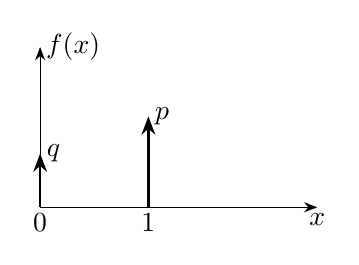
\begin{tikzpicture}[x=1.1cm,y=1.1cm,>=Stealth]
    \draw[->] (0,0) -- (0,1.85) node[right,inner sep=2pt] {$f(x)$};
    \draw[->] (0,0) -- (3.2,0) node[below,inner sep=2pt] {$x$};
    \draw[->,thick] (0,0) -- (0,0.62) node[right,inner sep=2pt] {$q$};
    \draw[->,thick] (1.25,0) -- (1.25,1.05) node[right,inner sep=2pt] {$p$};
    \node[below,inner sep=2pt] at (0,0) {0};
    \node[below,inner sep=2pt] at (1.25,0) {1};
  \end{tikzpicture}
  \caption{0-1 分布的密度函数}\label{fig:1.15}
\end{figure}

\bhead{2.\ 二项分布（Binomial\nobreak）}

二项分布 $B(n,p)$ 的随机变量结果共有 $n+1$ 种\nobreak：整数 $0\sim n$\nobreak。我们常常这样来理解它\nobreak：$n$ 次独立试验\nobreak，每次都是同分布的 0-1 试验\nobreak，取 1 和 0 的概率分别为 $p$ 和 $q$\nobreak，$n$ 次试验中 1 发生的总次数 $k$ 就是二项分布\nobreak。

\begin{list}{}{\leftmargin=8.5em\itemindent=-7em\itemsep=4pt\topsep=4pt\parsep=0pt}
  \item \makebox[6em][l]{分布律\nobreak：}\quad $\displaystyle P_n(k)=\binom{n}{k}p^kq^{n-k},\qquad k=0,1,2,\cdots,n,\quad p+q=1$
  \item \makebox[6em][l]{分布函数\nobreak：}\quad $\displaystyle F(x)=\sum_{k=0}^{n}\binom{n}{k}p^kq^{n-k}u(x-k)$
  \item \makebox[6em][l]{密度函数\nobreak：}\quad $\displaystyle f(x)=\sum_{k=0}^{n}\binom{n}{k}p^kq^{n-k}\delta(x-k)$
  \item \makebox[6em][l]{均值与方差\nobreak：}\quad $EX=np,\qquad \Var(X)=npq$
  \item \makebox[6em][l]{特征函数\nobreak：}\quad $\phi(v)=\bigl(p\eu^{\ju v}+q\bigr)^n$
\end{list}

二项分布随机变量是离散的\nobreak，它的取值概率是二项式的系数\nobreak，因而得名为二项分布\nobreak。该随机变量的密度函数由冲激组成\nobreak，如图~\ref{fig:1.16} 所示\nobreak。典型的二项分布有\nobreak：连续 $n$ 次掷币试验后正面的总数目\nobreak，$n$ 次独立二元检验中总的吻合次数\nobreak，长为 $n$ 的独立二进制数据串中 1 的总数\nobreak，等等\nobreak。

\begin{figure}[htbp]
  \centering
  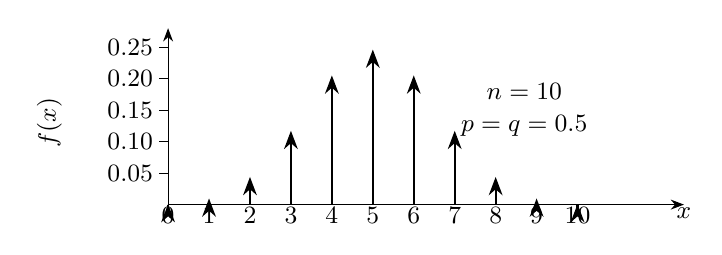
\begin{tikzpicture}[x=0.52cm,y=0.40cm,>=Stealth,font=\small]
    \draw[->] (0,0) -- (0,5.6);
    \node[rotate=90] at (-2.9,2.6) {$f(x)$};
    \draw[->] (0,0) -- (12.6,0) node[below,inner sep=1pt] {$x$};
    \foreach \y/\lab in {1/0.05,2/0.10,3/0.15,4/0.20,5/0.25}{%
      \draw (0,\y) -- (-0.22,\y) node[left,inner sep=2pt] {\lab};}
    \foreach \k/\h in {0/0.0195,1/0.1953,2/0.8789,3/2.3438,4/4.1016,5/4.9219,%
                       6/4.1016,7/2.3438,8/0.8789,9/0.1953,10/0.0195}{%
      \draw[->,thick] (\k,0) -- (\k,\h);}
    \foreach \k in {0,...,10}{\node[below,inner sep=1pt] at (\k,0) {\k};}
    \node at (8.7,3.6) {$n=10$};
    \node at (8.7,2.5) {$p=q=0.5$};
  \end{tikzpicture}
  \caption{二项分布的密度函数}\label{fig:1.16}
\end{figure}

\bhead{3.\ 泊松分布（Poisson\nobreak）}

泊松分布 $P(\lambda)$ 随机变量的结果为非负整数\nobreak。可这样理解\nobreak：在一个时段上某种事件可随机地发生许多次\nobreak，每次发生与否为独立同分布的 0-1 分布\nobreak，且单次发生的概率极小\nobreak，但总体而言平均发生的比率稳定在常数值 $\lambda$\nobreak，则发生的总次数 $k$ 是一个范围在 $[0,+\infty)$ 的整数随机变量\nobreak，其分布就是泊松分布\nobreak。特性如下\nobreak：

\begin{list}{}{\leftmargin=8.5em\itemindent=-7em\itemsep=4pt\topsep=4pt\parsep=0pt}
  \item \makebox[6em][l]{分布律\nobreak：}\quad $\displaystyle P(k)=\frac{\lambda^k}{k!}\eu^{-\lambda},\qquad k=0,1,2,\cdots,+\infty$
  \item \makebox[6em][l]{分布函数\nobreak：}\quad $\displaystyle F(x)=\sum_{k=0}^{\infty}\frac{\lambda^k}{k!}\eu^{-\lambda}u(x-k)$
  \item \makebox[6em][l]{密度函数\nobreak：}\quad $\displaystyle f(x)=\sum_{k=0}^{\infty}\frac{\lambda^k}{k!}\eu^{-\lambda}\delta(x-k)$
  \item \makebox[6em][l]{均值与方差\nobreak：}\quad $EX=\lambda,\qquad \Var(X)=\lambda$
  \item \makebox[6em][l]{特征函数\nobreak：}\quad $\phi(v)=\eu^{-\lambda(1-\eu^{\ju v})}$
\end{list}

泊松分布随机变量是离散的\nobreak，它的密度函数如图~\ref{fig:1.17} 所示\nobreak。大量的实际物理现象近似地符合这种分布\nobreak。例如\nobreak，顾客服务问题中\nobreak，顾客的数目\nobreak；误码发生问题中\nobreak，误码的数目\nobreak；网络服务器应用中\nobreak，服务请求的次数\nobreak；故障部件更换中\nobreak，更换的次数等\nobreak。

\begin{figure}[htbp]
  \centering
  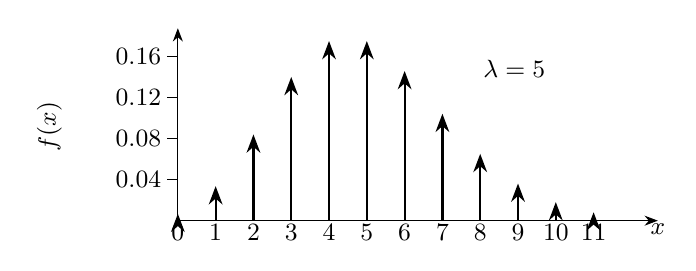
\begin{tikzpicture}[x=0.48cm,y=0.26cm,>=Stealth,font=\small]
    \draw[->] (0,0) -- (0,9.4);
    \node[rotate=90] at (-3.4,4.6) {$f(x)$};
    \draw[->] (0,0) -- (12.7,0) node[below,inner sep=1pt] {$x$};
    \foreach \y/\lab in {2/0.04,4/0.08,6/0.12,8/0.16}{%
      \draw (0,\y) -- (-0.28,\y) node[left,inner sep=2pt] {\lab};}
    \foreach \k/\h in {0/0.3369,1/1.6845,2/4.2112,3/7.0187,4/8.7734,5/8.7734,%
                       6/7.3111,7/5.2223,8/3.2639,9/1.8133,10/0.9067,11/0.4121}{%
      \draw[->,thick] (\k,0) -- (\k,\h);}
    \foreach \k in {0,...,11}{\node[below,inner sep=1pt] at (\k,0) {\k};}
    \node at (8.9,7.4) {$\lambda=5$};
  \end{tikzpicture}
  \caption{泊松分布的密度函数}\label{fig:1.17}
\end{figure}

\bhead{4.\ （离散\nobreak）均匀分布（Uniform\nobreak）}

（离散\nobreak）均匀分布是 $N$ 元等概的\nobreak，其概率特性如下\nobreak。

\begin{list}{}{\leftmargin=8.5em\itemindent=-7em\itemsep=4pt\topsep=4pt\parsep=0pt}
  \item \makebox[6em][l]{分布律\nobreak：}\quad $\displaystyle P(X=k)=\frac{1}{N},\qquad k=0,1,2,\cdots,N-1$
  \item \makebox[6em][l]{分布函数\nobreak：}\quad $\displaystyle F(x)=\sum_{k=0}^{N-1}\frac{1}{N}u(x-k)$
  \item \makebox[6em][l]{密度函数\nobreak：}\quad $\displaystyle f(x)=\sum_{k=0}^{N-1}\frac{1}{N}\delta(x-k)$
  \item \makebox[6em][l]{均值与方差\nobreak：}\quad $EX=\frac{N-1}{2},\qquad \Var(X)=\frac{N^2-1}{12}$
\end{list}

% EQNUMBERS: 1.67, 1.68
% FIGNUMBERS: 1.15, 1.16, 1.17   （图1.18 在书 p.28，不在本片段）

% =====================================================================
%  frag_I.tex  —— 《随机信号分析（第5版）》书 p.28 – p.30
%  内容：§1.6 典型分布（后半）：5.（连续）均匀分布 → 6. 指数分布
%        → 7. 正态（或高斯）分布（含 定理1.7 中心极限定理、误差/补误差/
%          Q(x) 函数）→ 8. 瑞利与莱斯分布 → 9. χ²分布（1）中心 χ² 分布
%        本片段为第1章正文的结尾（§1.7 仿真与习题按要求跳过）。
%  起始处承接书 p.27 页末（§1.6 第4项「（离散）均匀分布」的特征函数）。
%  编号：本片段第一个编号公式为 (1.69)。
%  ※ 注意：§1.6 的节标题（含 1.–4. 各分布）位于书 p.26–p.27，
%     不在本片段的页范围内，本片段未包含该 \section 标题。
%  ※ 图号：图1.18 – 图1.23 在本片段内（图1.18 原书在书 p.28 顶部，已补）；原注：
%     p.27）与图 1.11（瑞利与莱斯密度函数，p.15），二者不在本页范围内。
% =====================================================================

% ------- 承接自书 p.27：（离散）均匀分布的特征函数 -------
特征函数\nobreak：
\[
\phi(v)=\frac{1-\eu^{\ju Nv}}{N(1-\eu^{\ju v})}
\]

（离散\nobreak）均匀分布随机变量的密度函数如图 1.18 所示\nobreak。常常用到的古典概型就是（离散\nobreak）均匀分布的\nobreak。

\begin{figure}[htbp]
  \centering
  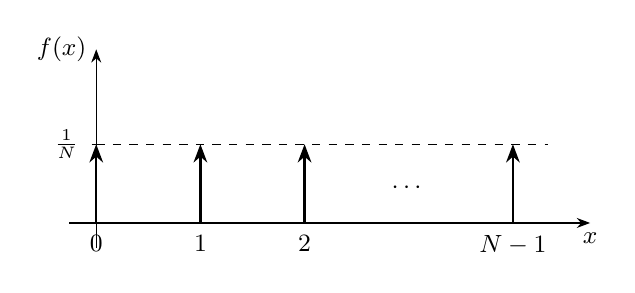
\begin{tikzpicture}[scale=0.98,>=Stealth,every node/.style={font=\small}]
    % 坐标轴
    \draw[->] (-0.35,0) -- (6.40,0) node[below] {$x$};
    \draw[->] (0,-0.32) -- (0,2.25) node[left] {$f(x)$};
    % 1/N 高度虚线
    \draw[dashed] (0,1.02) -- (5.85,1.02);
    \draw (-0.06,1.02) -- (0.06,1.02);
    \node[left] at (-0.10,1.02) {$\frac{1}{N}$};
    % 各点的冲激（幅度 1/N）
    \foreach \x in {0, 1.35, 2.70, 5.40}{
      \draw[thick,->] (\x,0) -- (\x,1.02);
    }
    % 横轴刻度标注
    \node[below] at (0,-0.04) {$0$};
    \node[below] at (1.35,-0.04) {$1$};
    \node[below] at (2.70,-0.04) {$2$};
    \node[below] at (5.40,-0.04) {$N-1$};
    % 中间的省略号
    \node at (4.05,0.46) {$\cdots$};
  \end{tikzpicture}
  \caption{（离散\nobreak）均匀分布的密度函数}
  \label{fig:1.18}
\end{figure}


\bhead{5.\ （连续\nobreak）均匀分布（Uniform\nobreak）}
\noindent
（连续\nobreak）均匀分布 $U(a,b)$ 的特性如下\nobreak。

分布函数\nobreak：
\[
F(x)=\begin{cases}
0, & x\leqslant a\\[2pt]
\dfrac{x-a}{b-a}, & a<x\leqslant b\\[2pt]
1, & x>b
\end{cases}
\]

\begin{wrapfigure}{r}{0.34\textwidth}
  \centering
  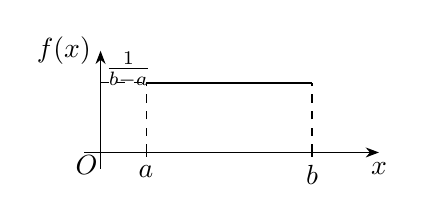
\begin{tikzpicture}[scale=0.68,>=Stealth]
    \draw[->] (-0.30,0) -- (5.20,0) node[below] {$x$};
    \draw[->] (0,-0.30) -- (0,1.90) node[left] {$f(x)$};
    \draw[thick] (0.85,1.30) -- (3.95,1.30);
    \draw[dashed] (0,1.30) -- (0.85,1.30);
    \draw[dashed] (0.85,0) -- (0.85,1.30);
    \draw[dashed] (3.95,0) -- (3.95,1.30);
    \draw (0.85,0) -- (0.85,-0.08);
    \draw (3.95,0) -- (3.95,-0.08);
    \node[below] at (0.85,-0.06) {$a$};
    \node[below] at (3.95,-0.06) {$b$};
    \node at (-0.26,-0.24) {$O$};
    \node at (0.52,1.54) {$\frac{1}{b-a}$};
  \end{tikzpicture}
  \caption{均匀分布的密度函数}
  \label{fig:1.19}
\end{wrapfigure}

密度函数\nobreak：
\[
f(x)=\begin{cases}
\dfrac{1}{b-a}, & a\leqslant x\leqslant b\\[2pt]
0, & \text{其他}
\end{cases}
\]

均值与方差\nobreak：\quad $EX=\dfrac{a+b}{2}$\nobreak，\quad $\Var(X)=\dfrac{(b-a)^2}{12}$

特征函数\nobreak：\quad $\phi(v)=\dfrac{\eu^{\ju bv}-\eu^{\ju av}}{\ju v(b-a)}$

均匀分布随机变量的密度函数如图 1.19 所示\nobreak。实际应用中\nobreak，均匀的或没有明确偏向性的物理特性导致均匀分布随机特性\nobreak。例如\nobreak，量化与截尾噪声一般认为具有均匀分布\nobreak，当步长为 $\Delta$ 时\nobreak，常认为量化与截尾噪声分别服从 $U(-\Delta/2,\Delta/2)$ 与 $U(0,\Delta)$\nobreak。此外\nobreak，工程中的正弦信号 $A\sin(\omega t+\Theta)$ 通常具有均匀的相位特性\nobreak，即 $\Theta\sim U(0,2\pi)$\nobreak。

\bhead{6.\ 指数分布（Exponential\nobreak）}
\noindent
指数分布随机变量的取值为非负实数\nobreak，具体特性如下（$\lambda>0$\nobreak）\nobreak。

分布函数\nobreak：
\[
F(x)=\begin{cases}
1-\eu^{-\lambda x}, & x\geqslant 0\\
0, & x<0
\end{cases}
\]

\begin{wrapfigure}{r}{0.32\textwidth}
  \centering
  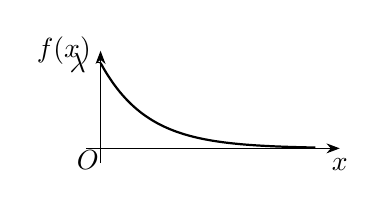
\begin{tikzpicture}[scale=0.62,>=Stealth]
    \draw[->] (-0.30,0) -- (4.90,0) node[below] {$x$};
    \draw[->] (0,-0.30) -- (0,2.00) node[left] {$f(x)$};
    \draw[thick] plot[domain=0:4.4,samples=80] (\x,{1.75*exp(-1.05*\x)});
    \draw (0,1.75) -- (-0.10,1.75);
    \node[left] at (-0.10,1.75) {$\lambda$};
    \node at (-0.26,-0.24) {$O$};
  \end{tikzpicture}
  \caption{指数分布的密度函数}
  \label{fig:1.20}
\end{wrapfigure}

密度函数\nobreak：
\[
f(x)=\begin{cases}
\lambda\eu^{-\lambda x}, & x\geqslant 0\\
0, & x<0
\end{cases}
\]

均值与方差\nobreak：\quad $EX=\dfrac{1}{\lambda}$\nobreak，\quad $\Var(X)=\dfrac{1}{\lambda^2}$

特征函数\nobreak：\quad $\phi(v)=\dfrac{1}{1-\ju v/\lambda}$

指数分布随机变量的密度函数如图 1.20 所示\nobreak。实际应用中它经常用于描述一些具有随机性的等待时间与间隔\nobreak。例如\nobreak，在公交车站等车的时间\nobreak；顾客排队等候服务的时间\nobreak；电话交换机或网络服务器等待呼叫的时间\nobreak；设备工作到出现故障的时间等\nobreak。指数分布与泊松分布密切关联\nobreak：事件的计数值是泊松的\nobreak，而事件的时间间隔正是指数型的\nobreak；反之亦然\nobreak。

\bhead{7.\ 正态（或高斯\nobreak）分布（Normal/Gaussian\nobreak）}
\noindent
正态（或高斯\nobreak）分布 $N(\mu,\sigma^2)$ 在概率论与统计学中有着重要地位\nobreak，它的具体特性如下\nobreak。

分布函数\nobreak：
\[
F(x)=\frac{1}{\sqrt{2\pi}\sigma}\int_{-\infty}^{x}\eu^{-(t-\mu)^2/2\sigma^2}\dif t
\]

\begin{wrapfigure}{r}{0.36\textwidth}
  \centering
  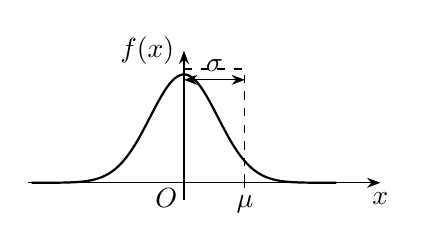
\begin{tikzpicture}[scale=0.86,>=Stealth]
    \draw[->] (-2.30,0) -- (2.90,0) node[below] {$x$};
    \draw[->] (0,-0.25) -- (0,1.95) node[left] {$f(x)$};
    \draw[thick] plot[domain=-2.25:2.25,samples=120]
      (\x,{1.60*exp(-2.0*\x*\x)});
    % σ 的标注： μ 到 μ+σ
    \draw[dashed] (0,1.68) -- (0.90,1.68);
    \draw[dashed] (0.90,0) -- (0.90,1.68);
    \draw[<->] (0,1.52) -- (0.90,1.52);
    \node[above] at (0.45,1.50) {$\sigma$};
    \draw (0.90,0) -- (0.90,-0.08);
    \node[below] at (0.90,-0.05) {$\mu$};
    \node at (-0.26,-0.22) {$O$};
  \end{tikzpicture}
  \caption{正态分布的密度函数}
  \label{fig:1.21}
\end{wrapfigure}

密度函数\nobreak：
\[
f(x)=\frac{1}{\sqrt{2\pi}\sigma}\eu^{-(x-\mu)^2/2\sigma^2}
\]

均值与方差\nobreak：\quad $EX=\mu$\nobreak，\quad $\Var(X)=\sigma^2$

特征函数\nobreak：\quad $\phi(v)=\eu^{\ju\mu v-\frac{\sigma^2v^2}{2}}$

正态分布随机变量的密度函数如图 1.21 所示\nobreak。在客观应用中的许多随机变量\nobreak，它们由大量相互独立的随机因素综合影响所形成\nobreak，而其中每一单个因素在总的影响中所起的作用是微小的\nobreak，这类随机变量大都近似地服从正态分布\nobreak。下面的中心极限定理（Central Limit Theorem\nobreak）给出了这种现象的数学解释\nobreak。

\thm{定理1.7}
设 $\{X_n\}$ 为独立同分布的随机变量序列\nobreak，记 $\mu=EX_n$\nobreak，$\sigma^2=\Var(X_n)$\nobreak，若 $\sigma^2<+\infty$\nobreak，则 $\displaystyle S_n=\sum_{i=1}^{n}X_i$ 满足
\begin{equation}
\lim_{n\to\infty}P\left\{\frac{S_n-n\mu}{\sigma\sqrt{n}}\leqslant x\right\}=\Phi(x)
\label{eq:1.69}
\end{equation}
式中\nobreak，$\displaystyle\Phi(x)=\int_{-\infty}^{x}\frac{1}{\sqrt{2\pi}}\eu^{-t^2/2}\dif t$ 是标准正态分布函数\nobreak。

我们经常需要查表计算正态分布 $F(x)$ 的数值\nobreak。为了计算方便\nobreak，人们编制了《标准正态分布表\nobreak》以供查阅\nobreak。标准正态分布函数为 $N(0,1)$\nobreak，记为 $\Phi(x)$\nobreak。易见 $\Phi(-x)=1-\Phi(x)$\nobreak，因此\nobreak，表有时只给出 $x\geqslant 0$ 的部分\nobreak。对于一般的正态分布 $X\sim N(\mu,\sigma^2)$\nobreak，有
\[
F(x)=\int_{-\infty}^{x}\frac{1}{\sqrt{2\pi}\sigma}\eu^{-\frac{(t-\mu)^2}{2\sigma^2}}\dif t=\Phi\left(\frac{x-\mu}{\sigma}\right)=\Phi(x)\ \text{表位于}\left(\frac{x-\mu}{\sigma}\right)\text{的值}
\]

应用中我们还常常用到与正态分布函数有关的其他几种函数\nobreak：

误差函数\nobreak：
\begin{equation}
\operatorname{erf}(x)=\frac{2}{\sqrt{\pi}}\int_{0}^{x}\eu^{-t^2}\dif t,\quad x\geqslant 0
\label{eq:1.70}
\end{equation}

补误差函数\nobreak：
\begin{equation}
\operatorname{erfc}(x)=\frac{2}{\sqrt{\pi}}\int_{x}^{\infty}\eu^{-t^2}\dif t,\quad x\geqslant 0
\label{eq:1.71}
\end{equation}

$Q(x)$ 函数\nobreak：
\begin{equation}
Q(x)=\frac{1}{\sqrt{2\pi}}\int_{x}^{\infty}\eu^{-t^2/2}\dif t
\label{eq:1.72}
\end{equation}

容易证明\nobreak，上述几个函数满足下面关系\nobreak：
\begin{equation}
\operatorname{erf}(x)=2\Phi(\sqrt{2}x)-1,\qquad \operatorname{erfc}(x)=2-2\Phi(\sqrt{2}x)
\label{eq:1.73}
\end{equation}
\begin{equation}
\operatorname{erf}(x)+\operatorname{erfc}(x)=1
\label{eq:1.74}
\end{equation}
\begin{equation}
Q(x)+\Phi(x)=1
\label{eq:1.75}
\end{equation}

误差\nobreak、补误差与 $Q(x)$ 函数的关系如图 1.22 所示\nobreak。

\begin{figure}[htbp]
  \centering
  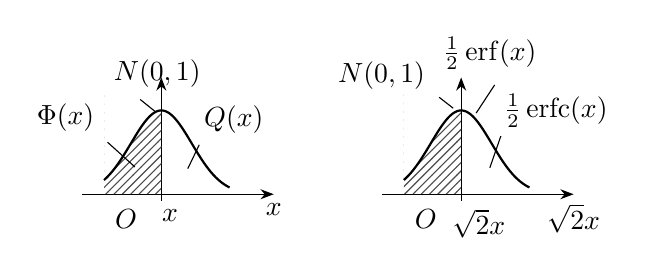
\begin{tikzpicture}[scale=0.56,>=Stealth]
    % ================= 左图：Φ(x) 与 Q(x) =================
    \begin{scope}[xshift=-3.40cm]
      \draw[->] (-0.20,0) -- (4.15,0) node[below] {$x$};
      \draw[->] (1.60,-0.15) -- (1.60,2.65);
      % Φ(x)：原点以左（阴影）
      \begin{scope}
        \clip (0.30,0) -- (0.30,2.50)
          -- plot[domain=0.30:1.60,samples=80]
             (\x,{1.90*exp(-1.05*(\x-1.60)*(\x-1.60))})
          -- (1.60,0) -- cycle;
        \fill[pattern=north east lines,pattern color=black!70] (0,0) rectangle (3.15,2.4);
      \end{scope}
      \draw[thick] plot[domain=0.30:3.15,samples=160]
        (\x,{1.90*exp(-1.05*(\x-1.60)*(\x-1.60))});
      \draw[dashed] (1.60,0) -- (1.60,1.90);
      \node[below] at (0.80,-0.12) {$O$};
      \node[below] at (1.80,-0.12) {$x$};
      \node[above right] at (0.30,2.20) {$N(0,1)$};
      \draw (1.12,2.15) -- (1.48,1.86);
      \node[anchor=south east] at (0.30,1.20) {$\Phi(x)$};
      \draw (0.38,1.18) -- (1.00,0.62);
      \node[anchor=south west] at (2.35,1.15) {$Q(x)$};
      \draw (2.46,1.12) -- (2.20,0.58);
    \end{scope}
    % ================= 右图：erf / erfc =================
    \begin{scope}[xshift=3.40cm]
      \draw[->] (-0.20,0) -- (4.15,0) node[below] {$\sqrt{2}x$};
      \draw[->] (1.60,-0.15) -- (1.60,2.65);
      % ½erf(x)：原点与 √2x 之间（阴影）
      \begin{scope}
        \clip (0.30,0) -- (0.30,2.50)
          -- plot[domain=0.30:1.60,samples=80]
             (\x,{1.90*exp(-1.05*(\x-1.60)*(\x-1.60))})
          -- (1.60,0) -- cycle;
        \fill[pattern=north east lines,pattern color=black!70] (0,0) rectangle (3.15,2.4);
      \end{scope}
      \draw[thick] plot[domain=0.30:3.15,samples=160]
        (\x,{1.90*exp(-1.05*(\x-1.60)*(\x-1.60))});
      \draw[dashed] (1.60,0) -- (1.60,1.90);
      \node[below] at (0.80,-0.12) {$O$};
      \node[below] at (2.00,-0.12) {$\sqrt{2}x$};
      \node[anchor=south east] at (1.00,2.15) {$N(0,1)$};
      \draw (1.10,2.20) -- (1.42,1.95);
      \node[above] at (2.25,2.60) {$\frac{1}{2}\operatorname{erf}(x)$};
      \draw (2.36,2.48) -- (1.94,1.84);
      \node[anchor=south west] at (2.35,1.30) {$\frac{1}{2}\operatorname{erfc}(x)$};
      \draw (2.50,1.32) -- (2.25,0.60);
    \end{scope}
  \end{tikzpicture}
  \caption{误差\nobreak、补误差与 $Q(x)$ 函数的关系}
  \label{fig:1.22}
\end{figure}

\bhead{8.\ 瑞利与莱斯分布（Rayleigh and Rician\nobreak）}
\noindent
瑞利与莱斯分布如 1.3.3 节所述\nobreak。它们是正态分布随机变量的变换结果\nobreak。

\noindent\textbf{（1\nobreak）瑞利分布}

\noindent
其取值为非负实数\nobreak，特性为\nobreak：

密度函数\nobreak：
\[
f(x)=\begin{cases}
\dfrac{x}{\sigma^2}\eu^{-\frac{x^2}{2\sigma^2}}, & x\geqslant 0\\[6pt]
0, & x<0
\end{cases}
\qquad(\sigma>0)
\]

均值与方差\nobreak：\quad $EX=\sqrt{\dfrac{\pi}{2}}\,\sigma$\nobreak，\quad $\Var(X)=(2-\pi/2)\sigma^2$

特征函数\nobreak：\quad $\phi(v)=\left(1+\ju\sqrt{\dfrac{\pi}{2}}\,\sigma v\right)\eu^{-\sigma^2v^2/2}$

\noindent\textbf{（2\nobreak）莱斯分布}

\noindent
其取值也为非负实数\nobreak，它的部分特性为\nobreak：

密度函数\nobreak：
\[
f(x)=\frac{x}{\sigma^2}\eu^{-(x^2+a^2)/2\sigma^2}I_0\left(\frac{ax}{\sigma^2}\right)\qquad(a>0,\sigma>0)
\]

式中\nobreak，$\displaystyle I_0(\eta)=\frac{1}{2\pi}\int_{0}^{2\pi}\eu^{\eta\cos\theta}\dif\theta$\nobreak。

均值\nobreak：
\[
EX=\left[(1+r)I_0\left(\frac{r}{2}\right)+rI_1\left(\frac{r}{2}\right)\right]\frac{\sqrt{\pi}}{2}\sigma\eu^{-\frac{r}{2}}
\]

式中\nobreak，$r=a^2/2\sigma^2$\nobreak，$I_1(\eta)$ 是修正的一阶贝塞尔函数（略\nobreak）\nobreak。

瑞利与莱斯分布随机变量的密度函数如图 1.11 所示\nobreak。它们在通信与电子工程领域的应用中经常出现\nobreak。例如\nobreak，后面将讨论的窄带高斯信号的包络就服从瑞利或莱斯分布\nobreak。

\bhead{9.\ $\chi^2$ 分布（Chi-square\nobreak）\nobreak：$\chi^2(n)$}
\noindent
$\chi^2$ 分布也是正态分布随机变量的变换结果\nobreak，它在统计检验中有重要的应用\nobreak。$\chi^2$ 分布又可以分为以下两种\nobreak。

\noindent\textbf{（1\nobreak）中心 $\chi^2$ 分布}

\noindent
$n$ 个独立\nobreak、零均值\nobreak、同方差的正态分布随机变量 $X_i\sim N(0,\sigma^2)$\nobreak，它们的平方和 $\displaystyle Y=\sum_{i=1}^{n}X_i^2$ 所具有的分布\nobreak，称为中心 $\chi^2$ 分布\nobreak，$n$ 是它的自由度\nobreak。其具体特性为\nobreak：

密度函数\nobreak：
\[
f(y)=\frac{y^{n/2-1}}{(2\sigma^2)^{n/2}\Gamma(n/2)}\eu^{-\frac{y}{2\sigma^2}},\quad y\geqslant 0
\]

式中\nobreak，$\displaystyle\Gamma(n/2)=\int_{0}^{\infty}x^{n/2-1}\eu^{-x}\dif x$\nobreak。

均值与方差\nobreak：\quad $EX=n\sigma^2$\nobreak，\quad $\Var(X)=2n\sigma^4$

特征函数\nobreak：\quad $\phi(v)=\left(1-\ju 2\sigma^2v\right)^{-n/2}$

\begin{wrapfigure}{r}{0.46\textwidth}
  \centering
  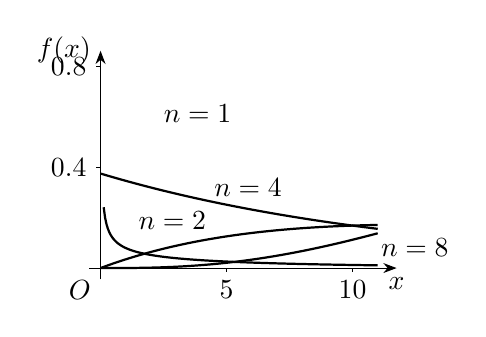
\begin{tikzpicture}[scale=0.80,>=Stealth]
    % 坐标轴：x: 0..11 → 0..4.40；f: 0..0.8 → 0..3.20
    \draw[->] (-0.18,0) -- (4.70,0) node[below] {$x$};
    \draw[->] (0,-0.18) -- (0,3.45) node[left] {$f(x)$};
    \draw (0,3.20) -- (-0.07,3.20);
    \node[left] at (-0.07,3.20) {$0.8$};
    \draw (0,1.60) -- (-0.07,1.60);
    \node[left] at (-0.07,1.60) {$0.4$};
    \node[below left] at (0,-0.04) {$O$};
    % n = 1
    \draw[thick] plot[domain=0.05:4.40,samples=200]
      (\x,{0.218/sqrt(\x)*exp(-0.2*\x)});
    % n = 2
    \draw[thick] plot[domain=0.0:4.40,samples=200]
      (\x,{1.50*exp(-0.2*\x)});
    % n = 4
    \draw[thick] plot[domain=0.0:4.40,samples=200]
      (\x,{0.375*\x*exp(-0.2*\x)});
    % n = 8
    \draw[thick] plot[domain=0.0:4.40,samples=200]
      (\x,{0.015625*\x*\x*\x*exp(-0.2*\x)});
    \node[anchor=west] at (0.85,2.45) {$n=1$};
    \node[anchor=south west] at (1.65,0.98) {$n=4$};
    \node[anchor=west] at (0.45,0.75) {$n=2$};
    \node[anchor=west] at (4.30,0.33) {$n=8$};
    \draw (2.00,0) -- (2.00,-0.07);
    \draw (4.00,0) -- (4.00,-0.07);
    \node[below] at (2.00,-0.05) {$5$};
    \node[below] at (4.00,-0.05) {$10$};
  \end{tikzpicture}
  \caption{中心 $\chi^2$ 分布的密度函数}
  \label{fig:1.23}
\end{wrapfigure}

中心 $\chi^2$ 分布随机变量的密度函数如图 1.23 所示\nobreak。

特别是 $n=2$ 时\nobreak，$f(y)=\dfrac{1}{2\sigma^2}\eu^{-\dfrac{y}{2\sigma^2}}$\nobreak，$y\geqslant 0$\nobreak，它是指数分布\nobreak，而 $\lambda=\dfrac{1}{2\sigma^2}$\nobreak。

% =====================================================================
% EQNUMBERS: 1.69, 1.70, 1.71, 1.72, 1.73, 1.74, 1.75   （连续，无跳号）
%   本片段（书 p.28–p.30）原书**仅**对上述 7 个公式给出编号，且均印在书 p.29；
%   书 p.28 与 p.30 的各个分布特性公式原书均**未编号**，故一律用 \[ \] 排版，
%   不占号。编译本片段前须把 equation 计数器置为 68（即起始编号 1.69 减 1）。
% FIGNUMBERS: 1.19, 1.20, 1.21, 1.22, 1.23   （连续，无跳号）
%   编译本片段前须把 figure 计数器置为 18（即起始编号 1.19 减 1）。
% 前一片段（书 p.25–p.27）末号应为 (1.68)，图末号应为 图1.18（离散均匀分布），
% 与此处衔接连续。
% =====================================================================

\clearpage
\exhead{习题}
% =====================================================================
%  frag_J.tex  —— 《随机信号分析（第5版）》书 p.33（页中「习题」起）– p.34
%  内容：习题 1.1 – 1.15（1.15 在书 p.34 末行开始，题面未完，余下部分在书 p.35，
%        按页界不在本片段范围内，故到「试求」为止）。
%  说明：书 p.33 上半为 §1.7「实验 3 统计分析」及其 MATLAB 输出，按用户要求跳过，
%        本片段自该页中部的「习题」标题之后（即题 1.1）开始。
%        习题区原书**不给**任何公式编号，故全部用 \[ \] 或行内 $...$，不占号。
%  EQNUMBERS: （无 —— 本片段不含任何编号公式）
%  FIGNUMBERS: （无 —— 本片段不含插图；题 1.15 引用的「图题 1.15」在书 p.35）
%  排版注记：题 1.1、1.2、1.5、1.10、1.11、1.14 的子问题在原书中为「(1)(2) 一行、
%        (3)(4) 一行」的两列排，故一律用 subq 环境。subq 为等宽两列的 p 列，
%        故题 1.10(1)、1.14(1) 两条较长文字会在自己那一列内折到第二行（原书因字号小、
%        行宽大，这两条都是单行）；其余子问题均为单行。单元格内首行与续行均不缩进。
%        题 1.6、1.7、1.12 的子问题在原书中是**竖排**（左缩进、各自单独成行），
%        故不用 subq，而是各自另起一段排版（本文段间距比原书略大，属排版差异）。
%        题 1.13、1.15 无子问题。
% =====================================================================

\exer{1.1}已知 $A,B,C$ 为样本空间上的三个事件\nobreak，试用 $A,B,C$ 的运算关系表示下列事件\nobreak：

\begin{subq}\setlength{\parindent}{0pt}
（1\nobreak）$A$ 发生\nobreak，$B$ 与 $C$ 不发生\nobreak； & （2\nobreak）$A,B,C$ 都发生\nobreak；\\
（3\nobreak）$A,B,C$ 中至少有一个发生\nobreak； & （4\nobreak）$A,B,C$ 不多于两个发生\nobreak。
\end{subq}

\exer{1.2}已知样本空间 $\Omega=\{1,2,\cdots,10\}$\nobreak，事件 $A=\{2,3,4\}$\nobreak，$B=\{3,4,5\}$\nobreak，$C=\{5,6,7\}$\nobreak，写出下列事件的表达式\nobreak：

\begin{subq}\setlength{\parindent}{0pt}
（1\nobreak）$\overline{A}\cup B$ & （2\nobreak）$\overline{A}\,\overline{B}$\\
（3\nobreak）$\overline{A(B\cup C)}$ & （4\nobreak）$\overline{A}\,\overline{B}\,\overline{C}$
\end{subq}

\exer{1.3}设随机试验 $E$ 是将一枚硬币抛两次\nobreak，观察 $H$——正面\nobreak、$T$——反面出现的情况\nobreak，试分析它的样本空间\nobreak、事件与概率\nobreak。

\exer{1.4}设 $A,B$ 与 $C$ 是建立在样本空间 $\Omega$ 上的事件\nobreak，试证明\nobreak：
\[
P(A\cup B\cup C)=P(A)+P(B)+P(C)-P(AB)-P(AC)-P(BC)+P(ABC)
\]

\exer{1.5}已知事件 $A,B$ 相互独立\nobreak，试证明\nobreak：

\begin{subq}\setlength{\parindent}{0pt}
（1\nobreak）$A$ 和 $\overline{B}$ 相互独立\nobreak； & （2\nobreak）$\overline{A}$ 和 $B$ 相互独立\nobreak；\\
（3\nobreak）$\overline{A}$ 和 $\overline{B}$ 相互独立\nobreak。
\end{subq}

\exer{1.6}有四批零件\nobreak，第一批有 $2\,000$ 个零件\nobreak，其中 $5\%$ 是次品\nobreak。第二批有 $500$ 个零件\nobreak，其中 $40\%$ 是次品\nobreak。第三批和第四批各有 $1\,000$ 个零件\nobreak，次品约占 $10\%$\nobreak。我们随机地选择一个批次\nobreak，并随机地取出一个零件\nobreak。求\nobreak：

（1\nobreak）所选零件为次品的概率是多少\nobreak？

（2\nobreak）发现次品后\nobreak，它来自第二批的概率是多少\nobreak？

\exer{1.7}一个电子系统为 $5$ 个用户服务\nobreak。若各用户独立地使用系统\nobreak，每个用户使用系统时\nobreak，系统输出功率为 $0.6\,\mathrm{W}$\nobreak，使用概率均为 $0.3$\nobreak。

（1\nobreak）求电子系统输出功率的概率分布\nobreak；

（2\nobreak）系统输出大于 $2\,\mathrm{W}$ 时\nobreak，系统过载\nobreak，求其过载的概率\nobreak。

\exer{1.8}有朋自远方来\nobreak，她乘火车\nobreak、轮船\nobreak、汽车或飞机来的概率分别是 $0.3,0.2,0.1$ 和 $0.4$\nobreak。如果她乘火车\nobreak、轮船或汽车来\nobreak，迟到的概率分别是 $0.25,0.4$ 和 $0.1$\nobreak，乘飞机来则不会迟到\nobreak。结果她迟到了\nobreak，问她最可能搭乘的是哪种交通工具\nobreak？

\exer{1.9}设随机试验 $X$ 的分布律为

\begin{center}
\renewcommand{\arraystretch}{1.35}
\begin{tabular}{c|c|c|c}
\hline
$X$ & $1$ & $2$ & $3$\\
\hline
$P$ & $0.2$ & $0.5$ & $0.3$\\
\hline
\end{tabular}
\end{center}

求 $X$ 的概率密度和分布函数\nobreak，并给出图形\nobreak。

\exer{1.10}设随机变量 $X$ 的绝对值不大于 $1$\nobreak，它在区间 $(-1,1)$ 上均匀分布\nobreak，且 $P(X=1)=0.2$\nobreak，$P(X=-1)=0.3$\nobreak。求\nobreak：

\begin{subq}\setlength{\parindent}{0pt}
（1\nobreak）$X$ 的概率密度和分布函数\nobreak，并给出图形\nobreak； & （2\nobreak）求 $P(X<0)$\nobreak。
\end{subq}

\exer{1.11}设随机变量 $X$ 的概率密度函数为 $f(x)=a\eu^{-\lvert x\rvert}$\nobreak，求\nobreak：

\begin{subq}\setlength{\parindent}{0pt}
（1\nobreak）系数 $a$\nobreak； & （2\nobreak）其分布函数\nobreak。
\end{subq}

\exer{1.12}某生产线制造 $1000\,\Omega$ 的电阻器\nobreak，必须满足容许偏差 $10\%$ 的要求\nobreak。实际生产的电阻器阻值不可能每次都是精确的 $1000\,\Omega$\nobreak，而是随机变化的\nobreak。实际生产电阻器阻值的概率分布满足 $N\bigl(1000,30^{2}\bigr)$\nobreak。求\nobreak：

（1\nobreak）该电阻器的报废率是多少\nobreak？

（2\nobreak）生产 $10^{6}$ 个电阻\nobreak，平均报废的电阻器是多少\nobreak？

\exer{1.13}某汽车站每天有 $1000$ 辆汽车进出\nobreak，而每辆汽车每天平均发生事故的概率为 $0.0001$\nobreak，问一天内汽车站出事故的次数大于 $1$ 的概率是多少\nobreak？

\exer{1.14}若离散随机变量 $X$ 与 $Y$ 的联合分布律如下\nobreak。试求\nobreak：

\begin{center}
\renewcommand{\arraystretch}{1.35}
\begin{tabular}{c|c|c|c}
\hline
\diagbox{$X$}{$Y$} & $-1$ & $0$ & $1$\\
\hline
$0$ & $0.07$ & $0.18$ & $0.15$\\
\hline
$1$ & $0.08$ & $0.32$ & $0.20$\\
\hline
\end{tabular}
\end{center}

\begin{subq}\setlength{\parindent}{0pt}
（1\nobreak）$X$ 与 $Y$ 的联合分布函数与密度函数\nobreak； & （2\nobreak）$X$ 与 $Y$ 的边缘分布律\nobreak；\\
（3\nobreak）$Z=XY$ 的分布律\nobreak； & （4\nobreak）$X$ 与 $Y$ 的相关系数\nobreak。
\end{subq}

\exer{1.15}设高斯随机变量 $X\sim N(0,2)$ 作用于一个 $L=4$ 电平的量化器\nobreak，其量化特性如图题 1.15 所示\nobreak。试求

% =====================================================================
%  frag_K.tex  —— 《随机信号分析（第5版）》书 p.35 – p.36（第1章 习题部分，收尾片段）
%  内容：习题 1.16 – 1.39（含书 p.34 末 1.15 题面的续写句）
%  ※ 本片段是第1章习题的最后一页半：书 p.36 页末（1.39 之后）习题结束，
%     故全书第1章习题止于 1.39。
%  ※ 开头的「输出随机变量 $Y$ 的分布律。」是书 p.35 第一行，即 p.34 末
%     1.15 题面「……其量化特性如图题 1.15 所示。试求」的续写。它**不是**
%     独立成题，故**不写** \exer{1.15}，只作承接段落。若 p.34 片段已抄这句，
%     合并时请二选一，避免重复（本片段保留它以保 1.15 题面完整可读）。
%  ※ 本片段内**没有**任何带编号的公式（原书习题一律不给公式号），
%     故全部用 \[ \] 或行内 $...$，不占 equation 号。
%  ※ 习题配图标为「图题 1.15」「图题 1.17」——这是**习题配图**，不属于正文
%     图1.x 系列，故**不用** figure 环境、**不用** \caption，也不动 figure 计数器；
%     用 center + tabular 并排 + 手工图注（图注文字照原书：图 题1.15 / 图 题1.17）。
%  ※ 排版说明（原书子问题布局与本片段的对应关系）：
%     · 1.16 → 原书竖排 (1)(2)，本片段亦竖排（分段）。
%     · 1.18 → 原书 (1)(2)(3) 紧凑相邻排于一行，本片段用 citemize 竖排单列。
%     · 1.23 / 1.28 / 1.32 / 1.33 → 原书两列排，本片段用 subq。
%     · 1.24 → 原书 (1)(2) 并列于一行，本片段用 subq 单行。
%     · 1.27 → 原书 (1)(2) 一行、(3)(4) 两行；本片段 subq 保持同样分组，
%       其中 (3) 单行、把 (4) 的 f(x) 放右列（(3) 行宽 313.9pt、(4) 行宽 205.8pt，
%       均超过 subq 单列可用宽 174.6pt，凡超宽者一律令其独占整行，避免折行）。
%     · 1.29 → 原书 (1)(2) 一行、(3)(4) 一行；(1) 行宽 291.5pt，与 (2) 并排必折行，
%       故本片段把 (1) 独占一行、(2)(3) 合并到一行、(4) 独占一行。
%     · 1.34 / 1.39 → 原书竖排，本片段用 citemize 竖排。
%  ※ 1.27 的 (1)(2) 印在书 p.35 页末、(3)(4) 印在 p.36 页首，系页面断行所致，
%     本片段合并为同一组 subq（(3)(4) 未另起 \exer）。
% =====================================================================

输出随机变量 $Y$ 的分布律\nobreak。

\exer{1.16}设随机变量 $X\sim N(0,1)$\nobreak，$Y\sim N(0,1)$\nobreak，且相互独立\nobreak，$U=X+Y$\nobreak，$V=X-Y$\nobreak。

（1\nobreak）求随机变量 $(U,V)$ 的联合概率密度 $f_{UV}(u,v)$\nobreak；

（2\nobreak）求随机变量 $U$ 与 $V$ 是否相互独立\nobreak？

\exer{1.17}半波整流器的输出 $Y$ 与输入 $X$ 之间的数学模型可以表示为
\[
Y=g(X)=\begin{cases}
X, & X\geqslant 0\\
0, & X<0
\end{cases}
\]
如图题 1.17 所示\nobreak。若已知输入随机变量 $X$ 的概率密度与分布函数分别为 $f_X(x)$ 和 $F_X(x)$\nobreak，试求输出 $Y$ 的概率密度函数 $f_Y(y)$\nobreak。

\begin{center}
\begin{tabular}{@{}c@{\hspace{0.02\textwidth}}c@{}}
\begin{tikzpicture}[x=0.70cm,y=0.62cm,>=stealth]
  % 习题配图「图题1.15」：L=4 电平的量化特性（阶梯）
  \draw[->] (-3.4,0) -- (3.5,0) node[right] {$X$};
  \draw[->] (0,-3.6) -- (0,3.85) node[above] {$Y$};
  \draw[thick] (-3.2,-3) -- (-2,-3);
  \draw[thick] (-2,-3) -- (-2,-1);
  \draw[thick] (-2,-1) -- (0,-1);
  \draw[thick] (0,-1) -- (0,1);
  \draw[thick] (0,1) -- (2,1);
  \draw[thick] (2,1) -- (2,3);
  \draw[thick] (2,3) -- (3.2,3);
  \draw[dashed] (0,1) -- (2,1);
  \draw[dashed] (2,0) -- (2,1);
  \draw (-0.08,1) -- (0.08,1);
  \draw (-0.08,2) -- (0.08,2);
  \draw (-0.08,3) -- (0.08,3);
  \draw (-0.08,-1) -- (0.08,-1);
  \draw (-0.08,-2) -- (0.08,-2);
  \draw (-0.08,-3) -- (0.08,-3);
  \draw (-2,0.1) -- (-2,-0.1);
  \draw (-1,0.1) -- (-1,-0.1);
  \draw (1,0.1) -- (1,-0.1);
  \draw (2,0.1) -- (2,-0.1);
  \node[left] at (-0.12,1) {$1$};
  \node[left] at (-0.12,2) {$2$};
  \node[left] at (-0.12,3) {$3$};
  \node[left] at (-0.12,-1) {$-1$};
  \node[left] at (-0.12,-2) {$-2$};
  \node[left] at (-0.12,-3) {$-3$};
  \node[below left] at (-2,-0.15) {$-2$};
  \node[below left] at (0,-0.15) {$0$};
  \node[below left] at (2,-0.15) {$2$};
\end{tikzpicture}
&
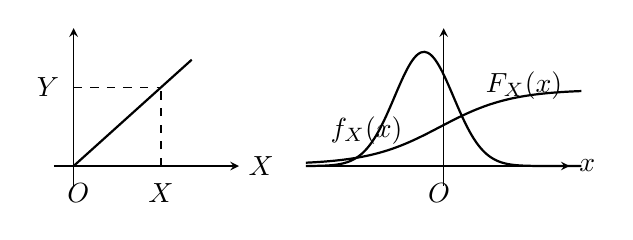
\begin{tikzpicture}[x=1.0cm,y=1.0cm,>=stealth]
  % 图题1.17：左为半波整流器特性 y=g(x)，右为 f_X(x) 与 F_X(x)
  \draw[->] (-0.25,0) -- (2.1,0) node[right] {$X$};
  \draw[->] (0,-0.25) -- (0,1.75);
  \draw[thick] (0,0) -- (1.5,1.35);
  \draw[dashed] (0,1.0) -- (1.11,1.0);
  \draw[dashed] (1.11,0) -- (1.11,1.0);
  \node[left] at (-0.06,1.0) {$Y$};
  \node[below] at (0.06,-0.1) {$O$};
  \node[below] at (1.11,-0.1) {$X$};
  % 右：f_X(x) 与 F_X(x)
  \begin{scope}[shift={(3.3,0)}]
    \draw[->] (-0.3,0) -- (3.0,0) node[right] {$x$};
    \draw[->] (1.4,-0.25) -- (1.4,1.75);
    \draw[thick] plot[smooth,domain=-0.35:3.15,samples=80] (\x,{1.45*exp(-(\x-1.15)*(\x-1.15)/0.28)});
    \draw[thick] plot[smooth,domain=-0.35:3.15,samples=80] (\x,{0.95/(1+exp(-2.2*(\x-1.35)))+0.02});
    \node at (0.42,0.45) {$f_X(x)$};
    \node at (2.42,1.02) {$F_X(x)$};
    \node[below] at (1.34,-0.1) {$O$};
  \end{scope}
\end{tikzpicture}
\\[2pt]
{\small 图\,题1.15} & {\small 图\,题1.17}
\end{tabular}
\end{center}

\exer{1.18}已知随机变量 $X$ 的可能取值为 $\{-4,-1,0,3,4\}$\nobreak，且每个值出现的概率均为 $1/5$\nobreak。求\nobreak：

\begin{citemize}
\item （1\nobreak）随机变量 $X$ 的数学期望和方差\nobreak；
\item （2\nobreak）随机变量 $Y=3X^2$ 的概率密度\nobreak；
\item （3\nobreak）$Y$ 的数学期望和方差\nobreak。
\end{citemize}

\exer{1.19}整数型随机变量 $X$ 与 $Y$ 独立\nobreak，密度函数分别为 $f_X(x)$ 与 $f_Y(y)$\nobreak，求 $X+Y$ 的分布\nobreak。

\exer{1.20}设服务器 L 由两个相互独立的子服务器 $\mathrm{L}_1$ 和 $\mathrm{L}_2$ 连接而成\nobreak，$\mathrm{L}_1,\mathrm{L}_2$ 的寿命 $X,Y$ 分别服从参数为 $\alpha,\beta$ 的指数分布\nobreak，两个子服务器的连接方式有\nobreak：（1\nobreak）串联\nobreak；（2\nobreak）并联\nobreak；（3\nobreak）备用\nobreak。试分别求出系统 L 寿命 $Z$ 的概率密度 $f_Z(z)$\nobreak。

\exer{1.21}随机变量 $X$ 与 $Y$ 中\nobreak，已知 $EX=1$\nobreak，$EY=3$\nobreak，$D(X)=4$\nobreak，$D(Y)=16$\nobreak，$\rho_{XY}=0.5$\nobreak，又设 $U=3X+Y$\nobreak，$V=X-2Y$\nobreak。试求 $EU$\nobreak，$EV$\nobreak，$D(U)$\nobreak，$D(V)$ 和 $\operatorname{Cov}(U,V)$\nobreak。

\exer{1.22}若随机变量 $X$ 与 $Y$ 的联合密度函数为
\[
f_{XY}(x,y)=\begin{cases}
xy/9, & 0\leqslant x<2,\ 0\leqslant y<3\\
0, & \text{其他}
\end{cases}
\]
判断 $X$ 与 $Y$ 是否正交\nobreak、无关与独立\nobreak。

\exer{1.23}若随机变量 $X$ 与 $Y$ 的联合密度函数为
\[
f_{XY}(x,y)=\begin{cases}
\eu^{-x}, & 0<y<x<1\\
0, & \text{其他}
\end{cases}
\]
求\nobreak：
\begin{subq}
（1\nobreak）$X$ 与 $Y$ 的边缘分布律\nobreak； & （2\nobreak）$X$ 与 $Y$ 的独立性\nobreak；\\
（3\nobreak）$E(Y|X=x)$\nobreak。 & \\
\end{subq}

\exer{1.24}已知随机变量 $X$ 服从 $[0,a]$ 上的均匀分布\nobreak，随机变量 $Y$ 服从 $[X,a]$ 上的均匀分布\nobreak。试求\nobreak：
\begin{subq}
（1\nobreak）$E(Y|X)$\nobreak，$0\leqslant X\leqslant a$\nobreak； & （2\nobreak）$EY$\nobreak。
\end{subq}

\exer{1.25}试证明条件期望基本性质\nobreak：$E[h(Y)g(X)|Y]=h(Y)E[g(X)|Y]$\nobreak。

\exer{1.26}设太空梭飞行中\nobreak，宇宙粒子进入其仪器舱的数目 $N$ 服从参数为 $\lambda$ 的泊松分布\nobreak。进舱后每个粒子造成损坏的概率为 $p$\nobreak，彼此独立\nobreak。求造成损坏的粒子的总数目\nobreak。

\exer{1.27}若随机变量 $X$ 的概率特性如下\nobreak，求其相应的特征函数\nobreak。
\begin{subq}
（1\nobreak）$X$ 为常数 $c$\nobreak，即 $P\{X=c\}=1$\nobreak； & （2\nobreak）参数为 2 的泊松分布\nobreak；\\
（3\nobreak）$(-1,1)$ 伯努利分布\nobreak：$f(x)=0.4\delta(x-1)+0.6\delta(x+1)$\nobreak； & \\
（4\nobreak）指数分布\nobreak： & $f(x)=\begin{cases}3\eu^{-3x}, & x\geqslant 0\\ 0, & \text{其他}\end{cases}$\nobreak。\end{subq}

\exer{1.28}随机变量 $X_1,X_2,X_3$ 彼此独立\nobreak，且特征函数分别为 $\phi_1(v)$\nobreak，$\phi_2(v)$\nobreak，$\phi_3(v)$\nobreak，求下列随机变量的特征函数\nobreak：
\begin{subq}
（1\nobreak）$X=X_1+X_2$\nobreak； & （2\nobreak）$X=X_1+X_2+X_3$\nobreak；\\
（3\nobreak）$X=X_1+2X_2+3X_3$\nobreak； & （4\nobreak）$X=2X_1+X_2+4X_3+10$\nobreak。
\end{subq}

\exer{1.29}随机变量 $X$ 具有下列特征函数\nobreak，求其概率密度函数\nobreak、均值\nobreak、均方值与方差\nobreak。
\begin{subq}
（1\nobreak）$\phi(v)=0.2+0.3\eu^{\ju 2v}+0.2\eu^{\ju 4v}+0.2\eu^{-\ju 2v}+0.1\eu^{-\ju 4v}$\nobreak； & \\
（2\nobreak）$\phi(v)=0.3\eu^{\ju v}+0.7\eu^{-\ju v}$\nobreak； & （3\nobreak）$\phi(v)=4/(4-\ju v)$\nobreak；\\
（4\nobreak）$\phi(v)=(\sin 5v)/(5v)$\nobreak。 & \\
\end{subq}

\exer{1.30}利用傅里叶变换推导均匀分布的特征函数\nobreak。

\exer{1.31}利用特征函数的唯一性\nobreak，证明\nobreak：若高斯随机变量 $X_i$\nobreak，$i=1,2,\cdots,n$\nobreak，$X_i\sim N(\mu_i,\sigma_i^2)$ 相互独立\nobreak，并且
\[
Y=\sum_{i=1}^{n}X_i
\]
则 $Y$ 也是高斯的\nobreak。

\exer{1.32}设有高斯随机变量 $X\sim N(\mu,\sigma^2)$\nobreak，试利用随机变量的矩发生特性证明\nobreak：
\begin{subq}
（1\nobreak）$EX=\mu$\nobreak； & （2\nobreak）$EX^2=\sigma^2+\mu^2$\nobreak；\\
（3\nobreak）$EX^3=3\mu\sigma^2+\mu^3$\nobreak。 & \\
\end{subq}

\exer{1.33}已知随机变量 $X,Y$ 的联合特征函数为
\[
\phi_{XY}(u,v)=\frac{6}{6-2\ju u-3\ju v-uv}
\]
求\nobreak：
\begin{subq}
（1\nobreak）随机变量 $X$ 的特征函数\nobreak； & （2\nobreak）随机变量 $Y$ 的期望和方差\nobreak。
\end{subq}

\exer{1.34}计算机在进行某种加法时\nobreak，将每个加数舍入最靠近它的整数\nobreak，假设所有舍入误差是独立的\nobreak，且在 $(-0.5,0.5)$ 服从均匀分布\nobreak。

\begin{citemize}
\item （1\nobreak）若将 1200 个数相加\nobreak，问误差总和的绝对值超过 10 的概率是多少\nobreak？
\item （2\nobreak）为保证误差总和的绝对值小于 10 的概率不小于 0.90\nobreak，最多可有几个数相加\nobreak？
\end{citemize}

\exer{1.35}编写 MATLAB 程序\nobreak，绘出 $N(3,0.5)$ 的概率密度和分布函数图形\nobreak。

\exer{1.36}编写 MATLAB 程序\nobreak，绘出二维正态分布 $N(0,1,2,0.5,0.3)$ 的概率密度函数和分布函数的图形\nobreak。

\exer{1.37}编写 MATLAB 程序\nobreak，绘出不同自由度的中心 $\chi^2$ 变量的概率密度函数\nobreak。

\exer{1.38}编写 MATLAB 程序\nobreak，求两组独立同分布的正态 $(N(0,2))$ 数据 $X$ 与 $Y$\nobreak，每组一万个分量\nobreak，即 $X=\{x_i\}$ 与 $Y=\{y_i\},i=1,2,\cdots,10000$\nobreak。令 $u_i=x_i^2+y_i^2$\nobreak，$z_i=\sqrt{u_i}$\nobreak，产生两组新数据 $U=\{u_i\}$ 与 $Z=\{z_i\}$\nobreak。试分析 $U$ 与 $Z$ 分别服从什么分布\nobreak，统计它们的均值并与分析结果对比\nobreak。

\exer{1.39}已知二维随机变量 $(X,Y)$ 的联合概率密度函数为
\[
f(x,y)=\begin{cases}
A\eu^{-(x+y)}, & x>0,\ y>0\\
0, & \text{其他}
\end{cases}
\]
利用 MATLAB 的符号运算功能\nobreak，求\nobreak：
\begin{subq}
（1\nobreak）待定系数 $A$\nobreak； & （2\nobreak）$P\{X>2,Y>1\}$\nobreak；\\
（3\nobreak）边缘分布 $f_X(x)$ 和 $f_Y(y)$\nobreak。 & \\
\end{subq}

% =====================================================================
% EQNUMBERS: 无（书 p.35–p.36 的习题原书**未给任何公式编号**，全部用 \[ \] 或行内公式）
% FIGNUMBERS: 无（习题配图「图题 1.15」「图题 1.17」不占用正文 图1.x 计数器；
%   本片段不含 figure 环境、不含 \caption，编译前后 figure 计数器不变）
% EXERCISES: 1.16 1.17 1.18 1.19 1.20 1.21 1.22 1.23 1.24 1.25 1.26 1.27
%            1.28 1.29 1.30 1.31 1.32 1.33 1.34 1.35 1.36 1.37 1.38 1.39
%   —— 逐个核对扫描件，**连续无跳号**（OCR 初稿漏掉的 1.21、1.34、1.36 实为识别遗漏，
%      书上确实存在）。最后一题：1.39，其后即为书 p.36 页码「· 36 ·」，习题结束。
% =====================================================================

\end{document}
